%!TeX spellcheck = en_EN
\newcommand\SLASH{\char`\\}

\newenvironment{dedication}{\vspace{6ex}\begin{quotation}\begin{center}\begin{em}}{\par\end{em}\end{center}\end{quotation}}

\documentclass{report}
\usepackage{tikz}
\usetikzlibrary{cd}
\usepackage{asymptote}
\usepackage{amsmath}
\usepackage{dsfont}
\usepackage{amssymb}
\usepackage{amsthm}
\usepackage{color}
\usepackage[toc,page]{appendix}
\usepackage[margin=1.1in]{geometry}

\usepackage{breqn}

\newcommand{\bimcell}{\draw[fill=blue!25] (-1,-1) -- (-1,0) -- (0,-1) -- cycle;
        			\draw[fill=blue!25] (1,-1) -- (1,0) -- (0,-1) -- cycle;
        			\draw[fill=blue!25] (-1,1) -- (-1,0) -- (0,1) -- cycle;
					\draw (1,1) -- (1,0);
					\draw (1,1) -- (0,1);}
					
\newcommand{\vertex}{\draw (0,0) -- (1,1);
					\draw (0,0) -- (1,0);
					\draw (0,0) -- (0,1);
					\draw (0,0) -- (-1,0);
					\draw (0,0) -- (0,-1);}
					
\newcommand{\ghostvertex}{\draw[gray] (0,0) -- (1,1);
					\draw[gray] (0,0) -- (1,0);
					\draw[gray] (0,0) -- (0,1);
					\draw[gray] (0,0) -- (-1,0);
					\draw[gray] (0,0) -- (0,-1);}
					
\newcommand{\redarrow}{\draw[fill=red!45] (0.07,0.07) -- (-0.07,0) -- (0,-0.07) -- cycle;}

\newcommand{\bigredarrow}{\draw[fill=red!45] (0.16,0.16) -- (-0.16,0) -- (0,-0.16) -- cycle;}

\newcommand{\greenarrow}{\draw[fill=green!45] (0.07,0.07) -- (-0.07,0) -- (0,-0.07) -- cycle;}

\newcommand{\biggreenarrow}{\draw[fill=green!45] (0.16,0.16) -- (-0.16,0) -- (0,-0.16) -- cycle;}

\newcommand{\interv}{0.12}

\newcommand{\triplegreenarrow}{
\draw[fill=green!45] (0.16-\interv , 0.16-\interv) -- (-0.16-\interv , 0-\interv) -- (0-\interv , -0.16-\interv) -- cycle;
\draw[fill=green!45] (0.16,0.16) -- (-0.16,0) -- (0,-0.16) -- cycle;
\draw[fill=green!45] (0.16+\interv , 0.16+\interv) -- (-0.16+\interv , 0+\interv) -- (0+\interv ,-0.16+\interv) -- cycle;}

\newcommand{\quadruplegreenarrow}{
\draw[fill=green!45] (0.16-1.5*\interv , 0.16-1.5*\interv) -- (-0.16-1.5*\interv , 0-1.5*\interv) -- (0-1.5*\interv , -0.16-1.5*\interv) -- cycle;
\draw[fill=green!45] (0.16-0.5*\interv , 0.16-0.5*\interv) -- (-0.16-0.5*\interv , 0-0.5*\interv) -- (0-0.5*\interv , -0.16-0.5*\interv) -- cycle;
\draw[fill=green!45] (0.16+0.5*\interv , 0.16+0.5*\interv) -- (-0.16+0.5*\interv , 0+0.5*\interv) -- (0+0.5*\interv , -0.16+0.5*\interv) -- cycle;
\draw[fill=green!45] (0.16+1.5*\interv , 0.16+1.5*\interv) -- (-0.16+1.5*\interv , 0+1.5*\interv) -- (0+1.5*\interv , -0.16+1.5*\interv) -- cycle;
}

\newcommand{\quintuplegreenarrow}{
\draw[fill=green!45] (0.16-2*\interv , 0.16-2*\interv) -- (-0.16-2*\interv , 0-2*\interv) -- (0-2*\interv , -0.16-2*\interv) -- cycle;
\draw[fill=green!45] (0.16-\interv , 0.16-\interv) -- (-0.16-\interv , 0-\interv) -- (0-\interv , -0.16-\interv) -- cycle;
\draw[fill=green!45] (0.16,0.16) -- (-0.16,0) -- (0,-0.16) -- cycle;
\draw[fill=green!45] (0.16+\interv , 0.16+\interv) -- (-0.16+\interv , 0+\interv) -- (0+\interv ,-0.16+\interv) -- cycle;
\draw[fill=green!45] (0.16+2*\interv , 0.16+2*\interv) -- (-0.16+2*\interv , 0+2*\interv) -- (0+2*\interv ,-0.16+2*\interv) -- cycle;}

\newcommand{\sextuplegreenarrow}{
\draw[fill=green!45] (0.16-2.5*\interv , 0.16-2.5*\interv) -- (-0.16-2.5*\interv , 0-2.5*\interv) -- (0-2.5*\interv , -0.16-2.5*\interv) -- cycle;
\draw[fill=green!45] (0.16-1.5*\interv , 0.16-1.5*\interv) -- (-0.16-1.5*\interv , 0-1.5*\interv) -- (0-1.5*\interv , -0.16-1.5*\interv) -- cycle;
\draw[fill=green!45] (0.16-0.5*\interv , 0.16-0.5*\interv) -- (-0.16-0.5*\interv , 0-0.5*\interv) -- (0-0.5*\interv , -0.16-0.5*\interv) -- cycle;
\draw[fill=green!45] (0.16+0.5*\interv , 0.16+0.5*\interv) -- (-0.16+0.5*\interv , 0+0.5*\interv) -- (0+0.5*\interv , -0.16+0.5*\interv) -- cycle;
\draw[fill=green!45] (0.16+1.5*\interv , 0.16+1.5*\interv) -- (-0.16+1.5*\interv , 0+1.5*\interv) -- (0+1.5*\interv , -0.16+1.5*\interv) -- cycle;
\draw[fill=green!45] (0.16+2.5*\interv , 0.16+2.5*\interv) -- (-0.16+2.5*\interv , 0+2.5*\interv) -- (0+2.5*\interv , -0.16+2.5*\interv) -- cycle;
}

\newcommand{\heptuplegreenarrow}{
\draw[fill=green!45] (0.16-3*\interv , 0.16-3*\interv) -- (-0.16-3*\interv , 0-3*\interv) -- (0-3*\interv , -0.16-3*\interv) -- cycle;
\draw[fill=green!45] (0.16-2*\interv , 0.16-2*\interv) -- (-0.16-2*\interv , 0-2*\interv) -- (0-2*\interv , -0.16-2*\interv) -- cycle;
\draw[fill=green!45] (0.16-\interv , 0.16-\interv) -- (-0.16-\interv , 0-\interv) -- (0-\interv , -0.16-\interv) -- cycle;
\draw[fill=green!45] (0.16,0.16) -- (-0.16,0) -- (0,-0.16) -- cycle;
\draw[fill=green!45] (0.16+\interv , 0.16+\interv) -- (-0.16+\interv , 0+\interv) -- (0+\interv ,-0.16+\interv) -- cycle;
\draw[fill=green!45] (0.16+2*\interv , 0.16+2*\interv) -- (-0.16+2*\interv , 0+2*\interv) -- (0+2*\interv ,-0.16+2*\interv) -- cycle;
\draw[fill=green!45] (0.16+3*\interv , 0.16+3*\interv) -- (-0.16+3*\interv , 0+3*\interv) -- (0+3*\interv ,-0.16+3*\interv) -- cycle;}

\newcommand{\octuplegreenarrow}{
\draw[fill=green!45] (0.16-3.5*\interv , 0.16-3.5*\interv) -- (-0.16-3.5*\interv , 0-3.5*\interv) -- (0-3.5*\interv , -0.16-3.5*\interv) -- cycle;
\draw[fill=green!45] (0.16-2.5*\interv , 0.16-2.5*\interv) -- (-0.16-2.5*\interv , 0-2.5*\interv) -- (0-2.5*\interv , -0.16-2.5*\interv) -- cycle;
\draw[fill=green!45] (0.16-1.5*\interv , 0.16-1.5*\interv) -- (-0.16-1.5*\interv , 0-1.5*\interv) -- (0-1.5*\interv , -0.16-1.5*\interv) -- cycle;
\draw[fill=green!45] (0.16-0.5*\interv , 0.16-0.5*\interv) -- (-0.16-0.5*\interv , 0-0.5*\interv) -- (0-0.5*\interv , -0.16-0.5*\interv) -- cycle;
\draw[fill=green!45] (0.16+0.5*\interv , 0.16+0.5*\interv) -- (-0.16+0.5*\interv , 0+0.5*\interv) -- (0+0.5*\interv , -0.16+0.5*\interv) -- cycle;
\draw[fill=green!45] (0.16+1.5*\interv , 0.16+1.5*\interv) -- (-0.16+1.5*\interv , 0+1.5*\interv) -- (0+1.5*\interv , -0.16+1.5*\interv) -- cycle;
\draw[fill=green!45] (0.16+2.5*\interv , 0.16+2.5*\interv) -- (-0.16+2.5*\interv , 0+2.5*\interv) -- (0+2.5*\interv , -0.16+2.5*\interv) -- cycle;
\draw[fill=green!45] (0.16+3.5*\interv , 0.16+3.5*\interv) -- (-0.16+3.5*\interv , 0+3.5*\interv) -- (0+3.5*\interv , -0.16+3.5*\interv) -- cycle;
}

\newcommand{\enneatuplegreenarrow}{
\draw[fill=green!45] (0.16-4*\interv , 0.16-4*\interv) -- (-0.16-4*\interv , 0-4*\interv) -- (0-4*\interv , -0.16-4*\interv) -- cycle;
\draw[fill=green!45] (0.16-3*\interv , 0.16-3*\interv) -- (-0.16-3*\interv , 0-3*\interv) -- (0-3*\interv , -0.16-3*\interv) -- cycle;
\draw[fill=green!45] (0.16-2*\interv , 0.16-2*\interv) -- (-0.16-2*\interv , 0-2*\interv) -- (0-2*\interv , -0.16-2*\interv) -- cycle;
\draw[fill=green!45] (0.16-\interv , 0.16-\interv) -- (-0.16-\interv , 0-\interv) -- (0-\interv , -0.16-\interv) -- cycle;
\draw[fill=green!45] (0.16,0.16) -- (-0.16,0) -- (0,-0.16) -- cycle;
\draw[fill=green!45] (0.16+\interv , 0.16+\interv) -- (-0.16+\interv , 0+\interv) -- (0+\interv ,-0.16+\interv) -- cycle;
\draw[fill=green!45] (0.16+2*\interv , 0.16+2*\interv) -- (-0.16+2*\interv , 0+2*\interv) -- (0+2*\interv ,-0.16+2*\interv) -- cycle;
\draw[fill=green!45] (0.16+3*\interv , 0.16+3*\interv) -- (-0.16+3*\interv , 0+3*\interv) -- (0+3*\interv ,-0.16+3*\interv) -- cycle;
\draw[fill=green!45] (0.16+4*\interv , 0.16+4*\interv) -- (-0.16+4*\interv , 0+4*\interv) -- (0+4*\interv ,-0.16+4*\interv) -- cycle;}

\newcommand{\rmatrix}{\draw[fill=yellow!35] (0,0) circle [radius=0.4cm];
   \node[color=black] {$\mathfrak{R}$};}
   
\newcommand{\fixededge}{\draw[fill=red!45] (0,0) circle [radius=0.16cm];}

\newcommand{\greendot}{\draw[fill=green!45] (0,0) circle [radius=0.16cm];}

\newcommand{\bump}{\draw[fill=cyan, opacity = 0.45, draw = none] (-0.3,-1) -- (-0.3,9) -- (0.3,9) -- (0.3,-1) -- cycle;}

\newcommand{\antibump}{\draw[fill=yellow, opacity = 0.45, draw = none] (-0.3,-1) -- (-0.3,9) -- (0.3,9) -- (0.3,-1) -- cycle;}

\newcommand{\domainwall}{\draw[fill=violet!50, opacity = 0.45, draw = none] (-0.3,-1) -- (-0.3,9) -- (0.3,9) -- (0.3,-1) -- cycle;}

\newcommand{\lindeca}{\draw[fill=orange!50, opacity = 0.45, draw = none] (0,0) -- (0,2) -- (2,2) -- (2,0) -- cycle;
\draw[fill=orange!50, opacity = 0.45, draw = none] (4,0) -- (4,2) -- (6,2) -- (6,0) -- cycle;
\draw[fill=orange!50, opacity = 0.45, draw = none] (8,0) -- (8,2) -- (9,2) -- (9,0) -- cycle;
\draw[fill=orange!50, opacity = 0.45, draw = none] (0,4) -- (0,6) -- (2,6) -- (2,4) -- cycle;
\draw[fill=orange!50, opacity = 0.45, draw = none] (4,4) -- (4,6) -- (6,6) -- (6,4) -- cycle;
\draw[fill=orange!50, opacity = 0.45, draw = none] (8,4) -- (8,6) -- (9,6) -- (9,4) -- cycle;
\draw[fill=orange!50, opacity = 0.45, draw = none] (0,8) -- (0,9) -- (2,9) -- (2,8) -- cycle;
\draw[fill=orange!50, opacity = 0.45, draw = none] (4,8) -- (4,9) -- (6,9) -- (6,8) -- cycle;
\draw[fill=orange!50, opacity = 0.45, draw = none] (8,8) -- (8,9) -- (9,9) -- (9,8) -- cycle;
}

\newcommand{\lindecb}{\draw[fill=red!50, opacity = 0.45, draw = none] (0,0) -- (0,2) -- (2,2) -- (2,0) -- cycle;
\draw[fill=red!50, opacity = 0.45, draw = none] (4,0) -- (4,2) -- (6,2) -- (6,0) -- cycle;
\draw[fill=red!50, opacity = 0.45, draw = none] (8,0) -- (8,2) -- (9,2) -- (9,0) -- cycle;
\draw[fill=red!50, opacity = 0.45, draw = none] (0,4) -- (0,6) -- (2,6) -- (2,4) -- cycle;
\draw[fill=red!50, opacity = 0.45, draw = none] (4,4) -- (4,6) -- (6,6) -- (6,4) -- cycle;
\draw[fill=red!50, opacity = 0.45, draw = none] (8,4) -- (8,6) -- (9,6) -- (9,4) -- cycle;
\draw[fill=red!50, opacity = 0.45, draw = none] (0,8) -- (0,9) -- (2,9) -- (2,8) -- cycle;
\draw[fill=red!50, opacity = 0.45, draw = none] (4,8) -- (4,9) -- (6,9) -- (6,8) -- cycle;
\draw[fill=red!50, opacity = 0.45, draw = none] (8,8) -- (8,9) -- (9,9) -- (9,8) -- cycle;
}

\usetikzlibrary{positioning}

\title{\sc Combinatorial metamaterials with multiple degrees of freedom\\
	{\small Institute of Physics, University of Amsterdam}}
\author{\large \sc Aleksi Bossart\\ Advisor: Corentin Coulais}
\date{\today}       

\begin{document}
\maketitle

\begin{abstract}
	We investigate a new class of multimodal mechanical metamaterials arising from tiling the plane with a single bimodal cell. We propose an alternative to the compatibility matrix description of the zero modes in the form of a vertex model based on the linearized geometric constraints. The associated R-matrix is a tensor of order 5 respecting the ice rule, which hints at integrability. Using this model, we describe the rich mechanism phenomenology of our material. In particular, we present multimodal metamaterials with a number of zero modes that remains constant with increasing system size, as well as peculiar linearly decaying modes. We validate our predictions using a combination of finite-element simulations and elasticity experiments.
\end{abstract}

\tableofcontents
		
\chapter{Tilings with a bimodal primitive cell}

\section{Motivation}


\section{Primitive cell geometry and index theorem}
	
			\begin{figure}[!ht]
				\centering{
				\scalebox{1}{
				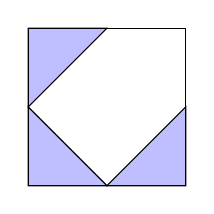
\begin{tikzpicture}
					\bimcell		
				\end{tikzpicture}
				}
				}
				\caption{The bimodal unit cell.}
				\label{fig:primitive}
			\end{figure}
			
	Repeating this primitive cell with arbitrary orientations on a Lieb lattice yields a variety of configurations. Our main purpose is to describe and classify the rich spectrum of elastic behaviour of these configurations.
			
			\begin{figure}[!ht]
				\centering{
				\scalebox{0.5}{
				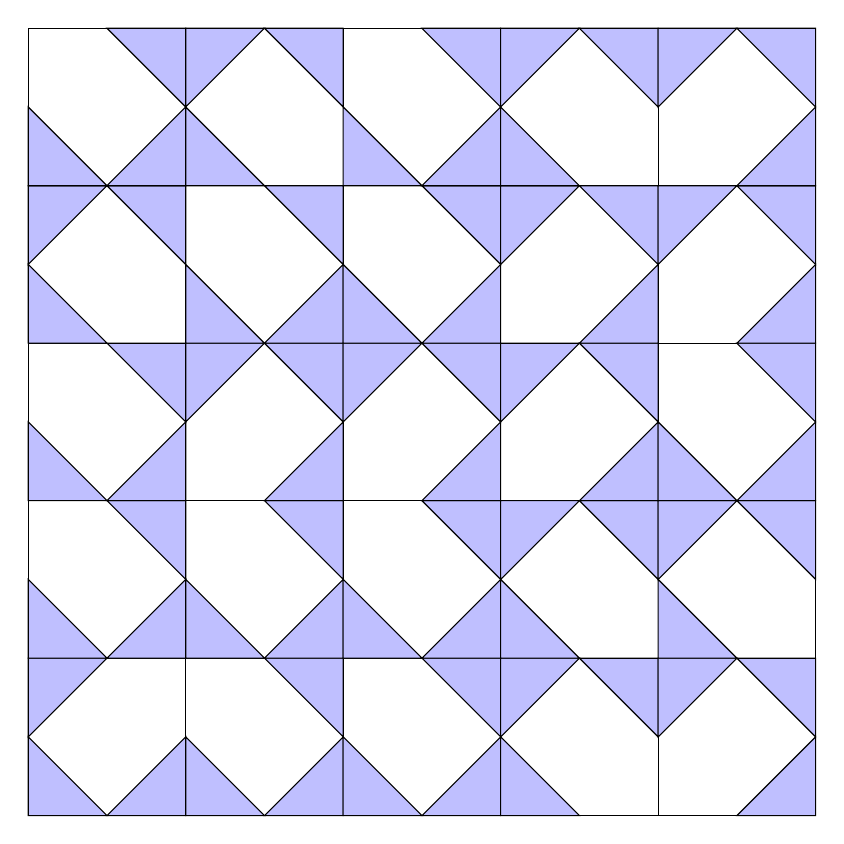
\begin{tikzpicture}
        				
					\bimcell

					\begin{scope}[xshift = 2cm, rotate = 90]
						\bimcell
					\end{scope}
					
					\begin{scope}[xshift = 4cm, rotate = 90]
						\bimcell
					\end{scope}

					\begin{scope}[xshift = 6cm, rotate = 270]
						\bimcell
					\end{scope}

					\begin{scope}[xshift = 8cm, rotate = 180]
						\bimcell
					\end{scope}
					
					\begin{scope}[yshift = 2cm, rotate = 90]
						\bimcell
					\end{scope}
					
					\begin{scope}[yshift = 2cm, xshift = 2cm, rotate = 90]
						\bimcell
					\end{scope}
					
					\begin{scope}[yshift = 2cm, xshift = 4cm, rotate = 90]
						\bimcell
					\end{scope}

					\begin{scope}[yshift = 2cm, xshift = 6cm, rotate = 270]
						\bimcell
					\end{scope}

					\begin{scope}[yshift = 2cm, xshift = 8cm, rotate = 270]
						\bimcell
					\end{scope}
					
					\begin{scope}[yshift = 4cm, rotate = 90]
						\bimcell
					\end{scope}
					
					\begin{scope}[yshift = 4cm, xshift = 2cm, rotate = 180]
						\bimcell
					\end{scope}
					
					\begin{scope}[yshift = 4cm, xshift = 4cm, rotate = 180]
						\bimcell
					\end{scope}

					\begin{scope}[yshift = 4cm, xshift = 6cm, rotate = 180]
						\bimcell
					\end{scope}

					\begin{scope}[yshift = 4cm, xshift = 8cm, rotate = 90]
						\bimcell
					\end{scope}
					
					\begin{scope}[yshift = 6cm, rotate = 270]
						\bimcell
					\end{scope}
					
					\begin{scope}[yshift = 6cm, xshift = 2cm, rotate = 90]
						\bimcell
					\end{scope}
					
					\begin{scope}[yshift = 6cm, xshift = 4cm, rotate = 90]
						\bimcell
					\end{scope}

					\begin{scope}[yshift = 6cm, xshift = 6cm, rotate = 180]
						\bimcell
					\end{scope}

					\begin{scope}[yshift = 6cm, xshift = 8cm, rotate = 180]
						\bimcell
					\end{scope}
					
					\begin{scope}[yshift = 8cm, rotate = 90]
						\bimcell
					\end{scope}
					
					\begin{scope}[yshift = 8cm, xshift = 2cm, rotate = 270]
						\bimcell
					\end{scope}
					
					\begin{scope}[yshift = 8cm, xshift = 4cm, rotate = 90]
						\bimcell
					\end{scope}

					\begin{scope}[yshift = 8cm, xshift = 6cm, rotate = 270]
						\bimcell				
					\end{scope}

					\begin{scope}[yshift = 8cm, xshift = 8cm, rotate = 180]
						\bimcell
					\end{scope}
										
				\end{tikzpicture}
				}
				}
				\caption{An arbitrary tiling with the bimodal unit cell.}
				\label{fig:tilinglieb}
			\end{figure}
			
	The Maxwell index theorem \cite{Indexthm} immediately provides us with a relation between the number of states of self-stress and the number of mechanisms,
			
			\begin{equation}
				dN-c = \frac{d(d+1)}{2}+N_M - N_{SS},
				\label{eq:indexthm}
			\end{equation}
			
			which we can evaluate for our pentagon-paved Lieb lattices. Each cell has a contribution of $N = 3$ and $c = 7$, with an additional contribution of $N = 2(n+m)+1$ and $c = 2(n+m)$ from the boundary. Constraining the displacements to a plane, this yields
			
			\begin{equation}
				N_M - N_{SS} = 2(3nm + 2(n+m) + 1) - (7nm + 2(n+m)) - 3 = 2(n+m) - nm - 1.
				\label{eq:periarea}
			\end{equation}


\chapter{An exotic vertex model}

	The bimodal nature of the above cell arises from purely geometrical considerations. To get a more quantitative theory, these geometric constraints can be encoded in three trigonometric equations. We then linearize these equations and represent the result graphically. This yields a nice design procedure, along with an exotic vertex model.
	
\section{Linearization of the geometric constraints}
\label{sec:derivegeometric}

			\begin{figure}[!ht]
				\centering{
				\scalebox{1}{
				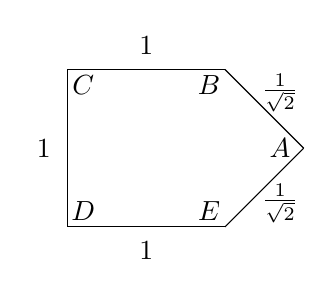
\begin{tikzpicture}
					\node[] at (-0.3,1) {1};
					\node[] at (1,2.3) {1};
					\node[] at (1,-0.3) {1};
					\node[] at (2.7,1.7) {$\frac{1}{\sqrt{2}}$};
					\node[] at (2.7,0.3) {$\frac{1}{\sqrt{2}}$};
					
					\node[] at (0.2,0.2) {$D$};
					\node[] at (1.8,0.2) {$E$};
					\node[] at (0.2,1.8) {$C$};
					\node[] at (1.8,1.8) {$B$};
					\node[] at (2.7,1) {$A$};

					\draw (0,0) -- (0,2);
					\draw (0,0) -- (2,0);
					\draw (2,2) -- (0,2);
					\draw (2,2) -- (3,1);
					\draw (2,0) -- (3,1);

				\end{tikzpicture}
				}}
				\caption{The prismatic pentagon in the reference position.}
				\label{fig:prismapent}
			\end{figure}
			
			Following \cite{PentaTrig}, the geometric constraints put forward by the side lengths of the pentagon can be expressed as\footnote{The complex number notation is much clearer, as usual.}
			
			\begin{equation}
				A+B+C+D+E = 3\pi,
				\label{eq:anglesum}
			\end{equation}
			
			\begin{equation}
				1 - \cos(A) = 3 - 2 \cos(C) - 2 \cos(D) + 2 \cos(C+D),
				\label{eq:cosinelaw}
			\end{equation}
			
			\begin{equation}
				\sin(D) - \frac{\sin(D+E)}{\sqrt{2}} = \sin(C) - \frac{\sin(C+B)}{\sqrt{2}}.
				\label{eq:sinelaw}
			\end{equation}
			
			We can linearize these expressions around the
			
			\begin{equation}
				A = \frac{\pi}{2} + \alpha\quad B = \frac{3\pi}{4} + \beta\quad C = \frac{\pi}{2} + \gamma\quad D = \frac{\pi}{2} + \delta\quad E = \frac{3\pi}{4} + \epsilon
				\label{eq:restangles}
			\end{equation}
			
			choice of angles, yielding the following system of linear equations,
			
			\begin{equation}
				\begin{pmatrix}
					1 & 1 & 1 & 1 & 1\\
					1 & -2 &  &  & -2\\
					 & 1 & 1 & -1 & -1
				\end{pmatrix}
				\begin{pmatrix}
					\alpha\\
					\delta\\
					\epsilon\\
					\beta\\
					\gamma
				\end{pmatrix}
				=\begin{pmatrix}
					0\\
					0\\
					0
				\end{pmatrix}
				\rightarrow
				\begin{pmatrix}
					\alpha\\
					\delta\\
					\epsilon
				\end{pmatrix}
				=
				\begin{pmatrix}
					-2 & -2\\
					-1 & -2\\
					 2 & 3
				\end{pmatrix}
				\begin{pmatrix}
					\beta\\
					\gamma
				\end{pmatrix}.
				\label{eq:system}
			\end{equation}
			
			As expected from the index theorem, there are two free parameters. We express this constraint graphically in Fig.\ref{fig:fundamentalvertices}, by drawing the two modes of our pentagon in a convenient basis. Any linear combination of those two vertices is thus also an acceptable vertex.
	
	
\section{Formulation of the vertex model}
\label{sec:formvertex}


				\begin{figure}[!ht]
				\centering{
				\scalebox{1.5}{
				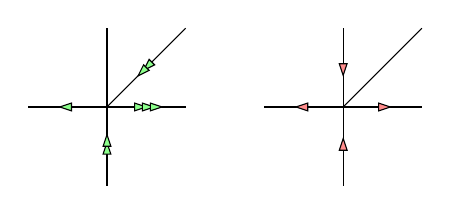
\begin{tikzpicture}
        				
					\vertex
					
					\begin{scope}[xshift = 0.535cm, yshift=0.535cm, rotate = 180]
						\greenarrow
					\end{scope}
					\begin{scope}[xshift = 0.465cm, yshift=0.465cm, rotate = 180]
						\greenarrow
					\end{scope}
					
					\begin{scope}[xshift = 0.4cm, yshift=0cm, rotate = -45]
						\greenarrow
					\end{scope}
					\begin{scope}[xshift = 0.5cm, yshift=0cm, rotate = -45]
						\greenarrow
					\end{scope}
					\begin{scope}[xshift = 0.6cm, yshift=0cm, rotate = -45]
						\greenarrow
					\end{scope}
					
					\begin{scope}[xshift = 0cm, yshift=-0.55cm, rotate = 45]
						\greenarrow
					\end{scope}
					\begin{scope}[xshift = 0cm, yshift=-0.45cm, rotate = 45]
						\greenarrow
					\end{scope}
					
					\begin{scope}[xshift = -0.5cm, yshift=0cm, rotate = 135]
						\greenarrow
					\end{scope}
					

					\begin{scope}[xshift = 3cm, rotate = 0]
						\vertex
					\end{scope}
					
					\begin{scope}[xshift = 3cm, yshift=0.5cm, rotate = -135]
						\redarrow
					\end{scope}
					
					\begin{scope}[xshift = 3.5cm, yshift=0cm, rotate = -45]
						\redarrow
					\end{scope}
					
					\begin{scope}[xshift = 3cm, yshift=-0.5cm, rotate = 45]
						\redarrow
					\end{scope}
					
					\begin{scope}[xshift = 2.5cm, yshift=0cm, rotate = 135]
						\redarrow
					\end{scope}
										
				\end{tikzpicture}
				}
				}
				\caption{Graphical representation of the linearized geometric constraints.}
				\label{fig:fundamentalvertices}
			\end{figure}
			
			Note that the red vertex in Fig.\ref{fig:fundamentalvertices} depicts a common finite mechanism\footnote{Set all the greek letter angles except $\chi$ in Eq.\ref{eq:gaugeangles} equal to zero and plug them in Eqs.\ref{eq:anglesum} to \ref{eq:sinelaw} to prove finiteness. Alternatively, squeeze the imaginary square in your head.}.

				\begin{figure}[!ht]
				\centering{
				\scalebox{0.5}{
				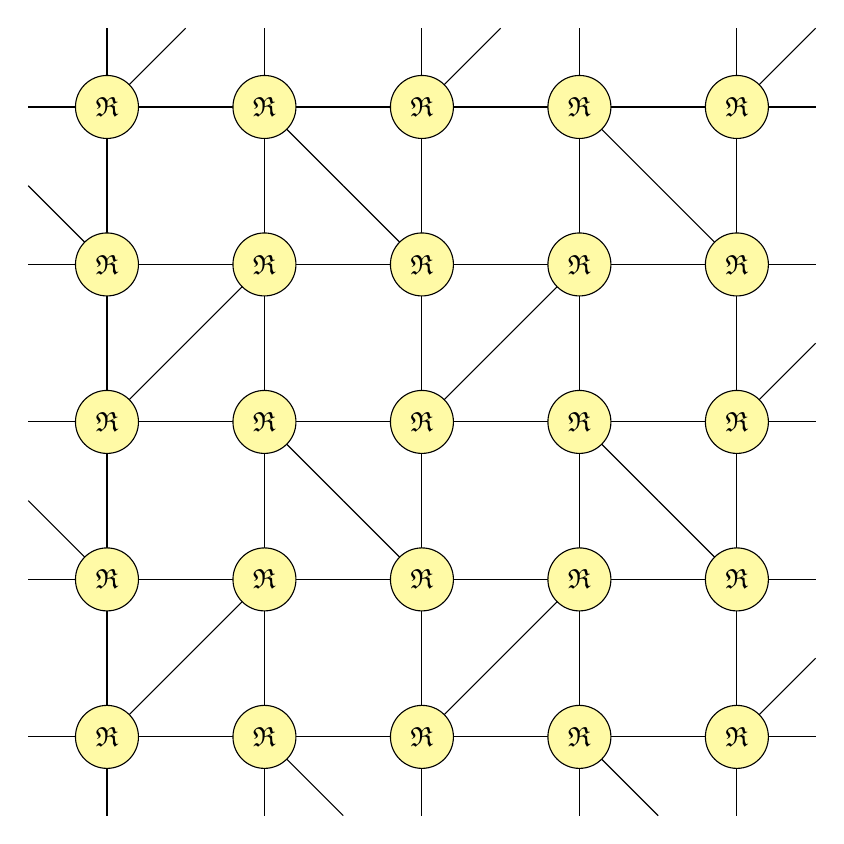
\begin{tikzpicture}
        				
					\vertex

					\begin{scope}[xshift = 2cm, rotate = 270]
						\vertex
					\end{scope}
					
					
					\begin{scope}[xshift = 4cm, rotate = 0]
						\vertex
					\end{scope}

					\begin{scope}[xshift = 6cm, rotate = 270]
						\vertex
					\end{scope}

					\begin{scope}[xshift = 8cm, rotate = 0]
						\vertex
					\end{scope}
					
					\begin{scope}[yshift = 2cm, rotate = 90]
						\vertex
					\end{scope}
					
					\begin{scope}[yshift = 2cm, xshift = 2cm, rotate = 180]
						\vertex
					\end{scope}
					
					\begin{scope}[yshift = 2cm, xshift = 4cm, rotate = 90]
						\vertex
					\end{scope}

					\begin{scope}[yshift = 2cm, xshift = 6cm, rotate = 180]
						\vertex
					\end{scope}

					\begin{scope}[yshift = 2cm, xshift = 8cm, rotate = 90]
						\vertex
					\end{scope}
					
					\begin{scope}[yshift = 4cm, rotate = 0]
						\vertex
					\end{scope}
					
					\begin{scope}[yshift = 4cm, xshift = 2cm, rotate = 270]
						\vertex
					\end{scope}
					
					\begin{scope}[yshift = 4cm, xshift = 4cm, rotate = 0]
						\vertex
					\end{scope}

					\begin{scope}[yshift = 4cm, xshift = 6cm, rotate = 270]
						\vertex
					\end{scope}

					\begin{scope}[yshift = 4cm, xshift = 8cm, rotate = 0]
						\vertex
					\end{scope}
					
					\begin{scope}[yshift = 6cm, rotate = 90]
						\vertex
					\end{scope}
					
					\begin{scope}[yshift = 6cm, xshift = 2cm, rotate = 180]
						\vertex
					\end{scope}
					
					\begin{scope}[yshift = 6cm, xshift = 4cm, rotate = 90]
						\vertex
					\end{scope}

					\begin{scope}[yshift = 6cm, xshift = 6cm, rotate = 180]
						\vertex
					\end{scope}

					\begin{scope}[yshift = 6cm, xshift = 8cm, rotate = 90]
						\vertex
					\end{scope}
					
					\begin{scope}[yshift = 8cm, rotate = 0]
						\vertex
					\end{scope}
					
					\begin{scope}[yshift = 8cm, xshift = 2cm, rotate = 270]
						\vertex
					\end{scope}
					
					\begin{scope}[yshift = 8cm, xshift = 4cm, rotate = 0]
						\vertex
					\end{scope}

					\begin{scope}[yshift = 8cm, xshift = 6cm, rotate = 270]
						\vertex
					\end{scope}

					\begin{scope}[yshift = 8cm, xshift = 8cm, rotate = 0]
						\vertex
					\end{scope}
					
					\rmatrix

					\begin{scope}[xshift = 2cm, rotate = 0]
						\rmatrix
					\end{scope}
					
					
					\begin{scope}[xshift = 4cm, rotate = 0]
						\rmatrix
					\end{scope}

					\begin{scope}[xshift = 6cm, rotate = 0]
						\rmatrix
					\end{scope}

					\begin{scope}[xshift = 8cm, rotate = 0]
						\rmatrix
					\end{scope}
					
					\begin{scope}[yshift = 2cm, rotate = 0]
						\rmatrix
					\end{scope}
					
					\begin{scope}[yshift = 2cm, xshift = 2cm, rotate = 0]
						\rmatrix
					\end{scope}
					
					\begin{scope}[yshift = 2cm, xshift = 4cm, rotate = 0]
						\rmatrix
					\end{scope}

					\begin{scope}[yshift = 2cm, xshift = 6cm, rotate = 0]
						\rmatrix
					\end{scope}

					\begin{scope}[yshift = 2cm, xshift = 8cm, rotate = 0]
						\rmatrix
					\end{scope}
					
					\begin{scope}[yshift = 4cm, rotate = 0]
						\rmatrix
					\end{scope}
					
					\begin{scope}[yshift = 4cm, xshift = 2cm, rotate = 0]
						\rmatrix
					\end{scope}
					
					\begin{scope}[yshift = 4cm, xshift = 4cm, rotate = 0]
						\rmatrix
					\end{scope}

					\begin{scope}[yshift = 4cm, xshift = 6cm, rotate = 0]
						\rmatrix
					\end{scope}

					\begin{scope}[yshift = 4cm, xshift = 8cm, rotate = 0]
						\rmatrix
					\end{scope}
					
					\begin{scope}[yshift = 6cm, rotate = 0]
						\rmatrix
					\end{scope}
					
					\begin{scope}[yshift = 6cm, xshift = 2cm, rotate = 0]
						\rmatrix
					\end{scope}
					
					\begin{scope}[yshift = 6cm, xshift = 4cm, rotate = 0]
						\rmatrix
					\end{scope}

					\begin{scope}[yshift = 6cm, xshift = 6cm, rotate = 0]
						\rmatrix
					\end{scope}

					\begin{scope}[yshift = 6cm, xshift = 8cm, rotate = 0]
						\rmatrix
					\end{scope}
					
					\begin{scope}[yshift = 8cm, rotate = 0]
						\rmatrix
					\end{scope}
					
					\begin{scope}[yshift = 8cm, xshift = 2cm, rotate = 0]
						\rmatrix
					\end{scope}
					
					\begin{scope}[yshift = 8cm, xshift = 4cm, rotate = 0]
						\rmatrix
					\end{scope}

					\begin{scope}[yshift = 8cm, xshift = 6cm, rotate = 0]
						\rmatrix
					\end{scope}

					\begin{scope}[yshift = 8cm, xshift = 8cm, rotate = 0]
						\rmatrix
					\end{scope}
										
				\end{tikzpicture}
				}
				}
				\caption{A network of contracted $\mathfrak{R}$-matrices.}
				\label{fig:vertexlindecay}
			\end{figure}
			
		The shape of the vertex indicates that the R-matrix should be a tensor of order 5. Futhermore, the linear combination freedom implies that the edge vector spaces are infinite. The ice rule is enforced (also in the full nonlinear theory) by the conserved sum of angles. A potentially successful formulation thus implies using an odd-dimensional multlinear operator as the R-matrix, with a kernel that respects our restricted ice rule in some way.
		
		By an angle-fixing argument, the model can be trivially extended to 6, 7 and 8 edges per vertex. Indeed, we can take our existing vertex and add a diagonal edge in either of the three available corners. If we then fix the value of one of these diagonal edges, we reduce the problem to the pentagonal case. Since this yields three independent vertices, it exhausts the available modes.
		
			
\section{Vertex configurations of fundamental mechanisms}
\label{sec:mechavertex}

	It is useful to describe the actuation of a few fundamental mechanisms in the vertex model framework, in order to understand the modes of the tilings described in the next chapter.

\subsection{Local building blocks}
\label{sec:legovertex}

	We will first consider all the possible \textit{contractions} of diagonal legs, since they give rise to the non-trivial modes. Considering the next-neighbour contraction of Fig.\ref{fig:hill}, we see that any choice of arrows on the left-hand vertex must be mirrored (with reversed directions) on the right-hand vertex.
			
			\begin{figure}[!ht]
				\centering{
				\scalebox{0.6}{
				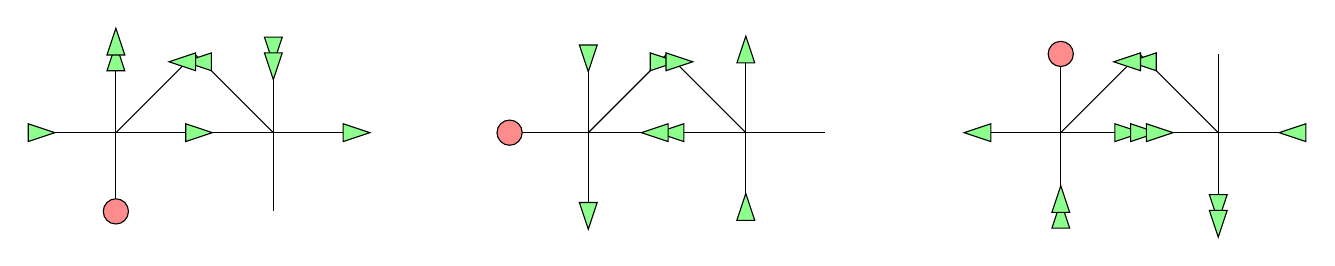
\begin{tikzpicture}
				
					\vertex
					\begin{scope}[yshift=-1cm]
						\fixededge
					\end{scope}
					\begin{scope}[xshift=-1cm, rotate = -45]
						\biggreenarrow
					\end{scope}
					\begin{scope}[yshift=0.9cm, rotate = 45]
						\biggreenarrow
					\end{scope}
					\begin{scope}[yshift=1.1cm, rotate = 45]
						\biggreenarrow
					\end{scope}
					
					%\node(1)[]{};
					%\node(2)[right = 1.8cm of 1]{};
				
					%\path[draw,thick]
					%(1) edge[out = 45, in = 135] node {} (2);
					
					\begin{scope}[xshift = 2cm, rotate = 90]
						\vertex
						\begin{scope}[xshift = -1cm]
							%\greendot
						\end{scope}
						
						\begin{scope}[xshift = 1.1cm, yshift=0cm, rotate = 135]
							\biggreenarrow
						\end{scope}
						\begin{scope}[xshift = 0.9cm, yshift=0cm, rotate = 135]
							\biggreenarrow
						\end{scope}
						\begin{scope}[xshift = 0.9cm, yshift=0.9cm, rotate = 45]
							\biggreenarrow
						\end{scope}
						\begin{scope}[xshift = 0.9cm, yshift=1.1cm, rotate = 45]
							\biggreenarrow
						\end{scope}
						\begin{scope}[yshift=1cm, rotate = -135]
							\biggreenarrow
						\end{scope}
						\begin{scope}[yshift=-1cm, rotate = -135]
							\biggreenarrow
						\end{scope}
					\end{scope}
					
					\begin{scope}[xshift = 6cm]
						\vertex
					\begin{scope}[xshift=-1cm]
						\fixededge
					\end{scope}
					\begin{scope}[yshift=-1cm, rotate = -135]
						\biggreenarrow
					\end{scope}
					\begin{scope}[yshift=1cm, rotate = -135]
						\biggreenarrow
					\end{scope}
					
					%\node(1)[]{};
					%\node(2)[right = 1.8cm of 1]{};
				
					%\path[draw,thick]
					%(1) edge[out = 45, in = 135] node {} (2);
					
					\begin{scope}[xshift = 2cm, rotate = 90]
						\vertex
						\begin{scope}[yshift = -1cm]
							%\greendot
						\end{scope}
						
						\begin{scope}[xshift = 1cm, yshift=0cm, rotate = -45]
							\biggreenarrow
						\end{scope}
						\begin{scope}[xshift = 0.9cm, yshift=1.1cm, rotate = -135]
							\biggreenarrow
						\end{scope}
						\begin{scope}[xshift = 0.9cm, yshift=0.9cm, rotate = -135]
							\biggreenarrow
						\end{scope}
						\begin{scope}[yshift=0.9cm, rotate = 45]
							\biggreenarrow
						\end{scope}
						\begin{scope}[yshift=1.1cm, rotate = 45]
							\biggreenarrow
						\end{scope}
						\begin{scope}[xshift=-1cm, rotate = -45]
							\biggreenarrow
						\end{scope}
					\end{scope}
					\end{scope}
					
					\begin{scope}[xshift = 12cm]
						\vertex
					\begin{scope}[yshift=1cm]
						\fixededge
					\end{scope}
					\begin{scope}[xshift=-1cm, rotate = 135]
						\biggreenarrow
					\end{scope}
					\begin{scope}[yshift=-1.1cm, rotate = 45]
						\biggreenarrow
					\end{scope}
					\begin{scope}[yshift=-0.9cm, rotate = 45]
						\biggreenarrow
					\end{scope}
					
					%\node(1)[]{};
					%\node(2)[right = 1.8cm of 1]{};
				
					%\path[draw,thick]
					%(1) edge[out = 45, in = 135] node {} (2);
					
					\begin{scope}[xshift = 2cm, rotate = 90]
						\vertex
						\begin{scope}[xshift = 1cm]
							%\greendot
						\end{scope}
						
						\begin{scope}[xshift = -0.9cm, yshift=0cm, rotate = 135]
							\biggreenarrow
						\end{scope}
						\begin{scope}[xshift = -1.1cm, yshift=0cm, rotate = 135]
							\biggreenarrow
						\end{scope}
						\begin{scope}[xshift = 0.9cm, yshift=0.9cm, rotate = 45]
							\biggreenarrow
						\end{scope}
						\begin{scope}[xshift = 0.9cm, yshift=1.1cm, rotate = 45]
							\biggreenarrow
						\end{scope}
						\begin{scope}[yshift=1.2cm, rotate = -135]
							\biggreenarrow
						\end{scope}
						\begin{scope}[yshift=1cm, rotate = -135]
							\biggreenarrow
						\end{scope}
						\begin{scope}[yshift=0.8cm, rotate = -135]
							\biggreenarrow
						\end{scope}
						\begin{scope}[yshift=-1cm, rotate = 45]
							\biggreenarrow
						\end{scope}
					\end{scope}
					\end{scope}
								
				\end{tikzpicture}
				}
				}
				\caption{The three non-trivial vertex configurations of a next-neighbour contraction.}
				\label{fig:hill}
			\end{figure}
			
	The next contraction possibility is a next-to-next-neighbour interaction, as depicted in Fig.\ref{fig:nnblock:2}. There are more available configurations, since a simple contraction is less demanding than a double.
	
		\begin{figure}[!ht]
				\centering{
				\scalebox{0.6}{
				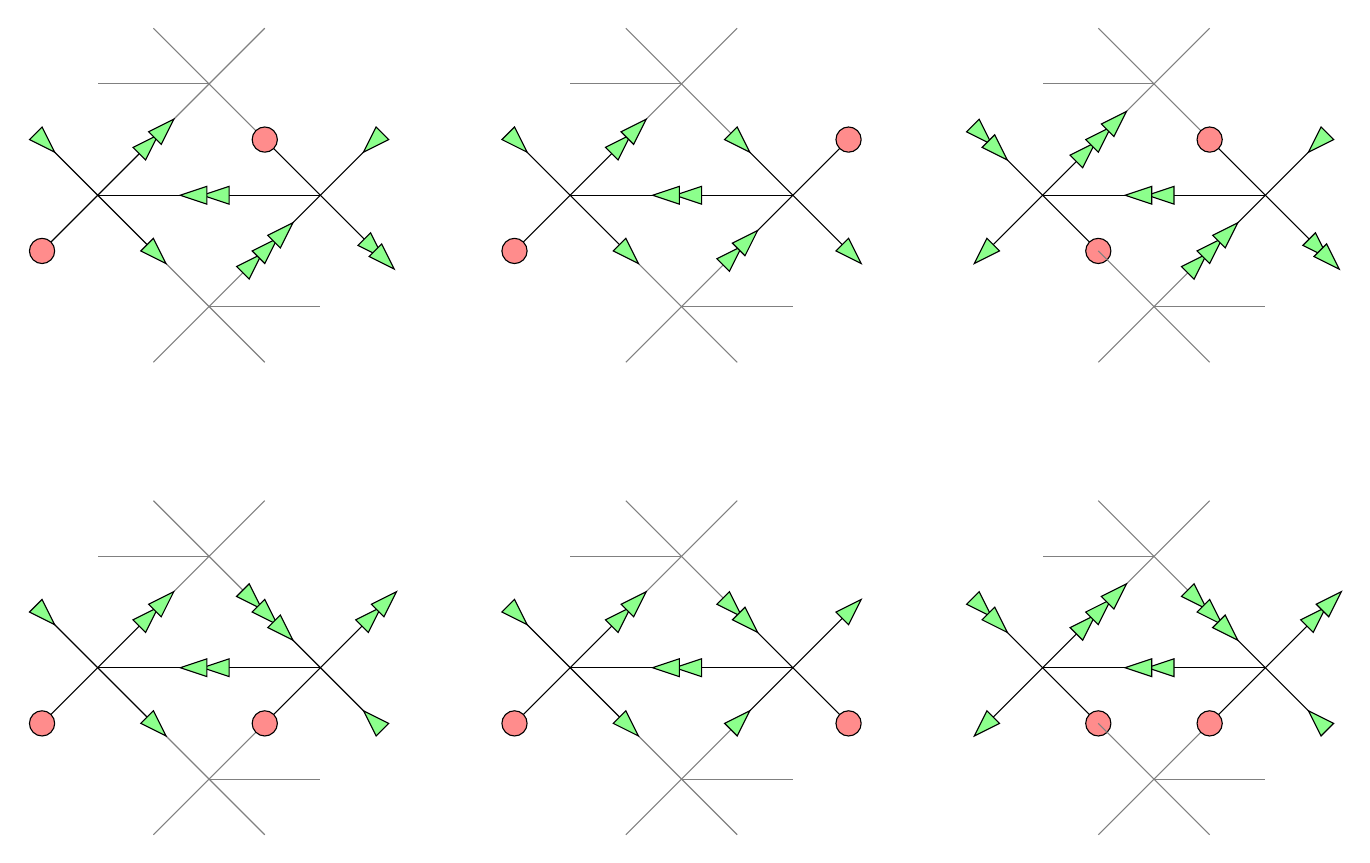
\begin{tikzpicture}
				
				\begin{scope}[xshift=0cm, yshift=0cm, rotate = -45]
					\begin{scope}[yshift = 2cm, rotate = 180]
						\ghostvertex
					\end{scope}
					
					\begin{scope}[yshift = 2cm, xshift = 2cm, rotate = 180]
						\vertex
						\begin{scope}[xshift = -0.9cm, yshift=0cm, rotate = 135]
							\biggreenarrow
						\end{scope}
						\begin{scope}[xshift = -1.1cm, yshift=0cm, rotate = 135]
							\biggreenarrow
						\end{scope}
						\begin{scope}[yshift = -1cm, yshift=0cm, rotate = 45]
							\biggreenarrow
						\end{scope}
					\end{scope}
        				
					\vertex
						\begin{scope}[yshift = -1cm, rotate = 0]
							\fixededge
						\end{scope}
						\begin{scope}[xshift = -1cm, yshift=0cm, rotate = -45]
							\biggreenarrow
						\end{scope}
						\begin{scope}[xshift = 0cm, yshift=0.86cm, rotate = 45]
							\biggreenarrow
						\end{scope}
						\begin{scope}[xshift = 0cm, yshift=1.14cm, rotate = 45]
							\biggreenarrow
						\end{scope}

					\begin{scope}[xshift = 2cm, rotate = 0]
						\ghostvertex
						\begin{scope}[yshift = 2cm, xshift=-1cm, rotate = 0]
							\fixededge
						\end{scope}
						\begin{scope}[xshift = -1cm, yshift=0cm, rotate = -45]
							\biggreenarrow
						\end{scope}
						\begin{scope}[xshift = -0.9cm, yshift=1.1cm, rotate = 180]
							\biggreenarrow
						\end{scope}
						\begin{scope}[xshift = -1.1cm, yshift=0.9cm, rotate = 180]
							\biggreenarrow
						\end{scope}
						\begin{scope}[xshift = 0cm, yshift=0.72cm, rotate = 45]
							\biggreenarrow
						\end{scope}
						\begin{scope}[xshift = 0cm, yshift=1cm, rotate = 45]
							\biggreenarrow
						\end{scope}
						\begin{scope}[xshift = 0cm, yshift=1.28cm, rotate = 45]
							\biggreenarrow
						\end{scope}
					\end{scope}
				\end{scope}
				
				
				
				
				 \begin{scope}[xshift=6cm, rotate = -45]
					\begin{scope}[yshift = 2cm, rotate = 180]
						\ghostvertex
					\end{scope}
					
					\begin{scope}[yshift = 2cm, xshift = 2cm, rotate = 180]
						\vertex
						\begin{scope}[xshift = 1cm, yshift=0cm, rotate = 135]
							\biggreenarrow
						\end{scope}
						\begin{scope}[xshift = -1cm, yshift=0cm, rotate = 135]
							\biggreenarrow
						\end{scope}
					\end{scope}
        				
					\vertex
						\begin{scope}[yshift = -1cm, rotate = 0]
							\fixededge
						\end{scope}
						\begin{scope}[xshift = -1cm, yshift=0cm, rotate = -45]
							\biggreenarrow
						\end{scope}
						\begin{scope}[xshift = 0cm, yshift=0.86cm, rotate = 45]
							\biggreenarrow
						\end{scope}
						\begin{scope}[xshift = 0cm, yshift=1.14cm, rotate = 45]
							\biggreenarrow
						\end{scope}

					\begin{scope}[xshift = 2cm, rotate = 0]
						\ghostvertex
						\begin{scope}[yshift = 3cm, rotate = 0]
							\fixededge
						\end{scope}
						\begin{scope}[xshift = -1cm, yshift=0cm, rotate = -45]
							\biggreenarrow
						\end{scope}
						\begin{scope}[xshift = -0.9cm, yshift=1.1cm, rotate = 180]
							\biggreenarrow
						\end{scope}
						\begin{scope}[xshift = -1.1cm, yshift=0.9cm, rotate = 180]
							\biggreenarrow
						\end{scope}
						\begin{scope}[xshift = 0cm, yshift=0.86cm, rotate = 45]
							\biggreenarrow
						\end{scope}
						\begin{scope}[xshift = 0cm, yshift=1.14cm, rotate = 45]
							\biggreenarrow
						\end{scope}
					\end{scope}
				\end{scope}
				
				
				
				
				
				\begin{scope}[xshift=12cm, rotate = -45]
					\begin{scope}[yshift = 2cm, rotate = 180]
						\ghostvertex
					\end{scope}
					
					\begin{scope}[yshift = 2cm, xshift = 2cm, rotate = 180]
						\vertex
						\begin{scope}[xshift = -0.9cm, yshift=0cm, rotate = 135]
							\biggreenarrow
						\end{scope}
						\begin{scope}[xshift = -1.1cm, yshift=0cm, rotate = 135]
							\biggreenarrow
						\end{scope}
						\begin{scope}[yshift = -1cm, yshift=0cm, rotate = 45]
							\biggreenarrow
						\end{scope}
					\end{scope}
        				
					\vertex
						\begin{scope}[xshift = 1cm, rotate = 0]
							\fixededge
						\end{scope}
						\begin{scope}[xshift = -1.14cm, yshift=0cm, rotate = -45]
							\biggreenarrow
						\end{scope}
						\begin{scope}[xshift = -0.86cm, yshift=0cm, rotate = -45]
							\biggreenarrow
						\end{scope}
						\begin{scope}[xshift = 0cm, yshift=0.72cm, rotate = 45]
							\biggreenarrow
						\end{scope}
						\begin{scope}[xshift = 0cm, yshift=1cm, rotate = 45]
							\biggreenarrow
						\end{scope}
						\begin{scope}[xshift = 0cm, yshift=1.28cm, rotate = 45]
							\biggreenarrow
						\end{scope}
						\begin{scope}[xshift = 0cm, yshift=-1cm, rotate = -135]
							\biggreenarrow
						\end{scope}

					\begin{scope}[xshift = 2cm, rotate = 0]
						\ghostvertex
						\begin{scope}[yshift = 2cm, xshift=-1cm, rotate = 0]
							\fixededge
						\end{scope}
						\begin{scope}[xshift = -0.9cm, yshift=1.1cm, rotate = 180]
							\biggreenarrow
						\end{scope}
						\begin{scope}[xshift = -1.1cm, yshift=0.9cm, rotate = 180]
							\biggreenarrow
						\end{scope}
						\begin{scope}[xshift = 0cm, yshift=0.72cm, rotate = 45]
							\biggreenarrow
						\end{scope}
						\begin{scope}[xshift = 0cm, yshift=1cm, rotate = 45]
							\biggreenarrow
						\end{scope}
						\begin{scope}[xshift = 0cm, yshift=1.28cm, rotate = 45]
							\biggreenarrow
						\end{scope}
					\end{scope}
				\end{scope}
				
				
				
				
				
				\begin{scope}[yshift=-6cm, xshift=0cm, rotate = -45]
					\begin{scope}[yshift = 2cm, rotate = 180]
						\ghostvertex
					\end{scope}
					
					\begin{scope}[yshift = 2cm, xshift = 2cm, rotate = 180]
						\vertex
						\begin{scope}[xshift = 1.28cm, yshift=0cm, rotate = 135]
							\biggreenarrow
						\end{scope}
						\begin{scope}[xshift = 1cm, yshift=0cm, rotate = 135]
							\biggreenarrow
						\end{scope}
						\begin{scope}[xshift = 0.72cm, yshift=0cm, rotate = 135]
							\biggreenarrow
						\end{scope}
						\begin{scope}[xshift = -1cm, yshift=0cm, rotate = -45]
							\biggreenarrow
						\end{scope}
						\begin{scope}[yshift = -0.86cm, yshift=0cm, rotate = -135]
							\biggreenarrow
						\end{scope}
						\begin{scope}[yshift = -1.14cm, yshift=0cm, rotate = -135]
							\biggreenarrow
						\end{scope}
					\end{scope}
        				
					\vertex
						\begin{scope}[yshift = -1cm, rotate = 0]
							\fixededge
						\end{scope}
						\begin{scope}[xshift = -1cm, yshift=0cm, rotate = -45]
							\biggreenarrow
						\end{scope}
						\begin{scope}[xshift = 0cm, yshift=0.86cm, rotate = 45]
							\biggreenarrow
						\end{scope}
						\begin{scope}[xshift = 0cm, yshift=1.14cm, rotate = 45]
							\biggreenarrow
						\end{scope}

					\begin{scope}[xshift = 2cm, rotate = 0]
						\ghostvertex
						\begin{scope}[yshift = 1cm, rotate = 0]
							\fixededge
						\end{scope}
						\begin{scope}[xshift = -1cm, yshift=0cm, rotate = -45]
							\biggreenarrow
						\end{scope}
						\begin{scope}[xshift = -0.9cm, yshift=1.1cm, rotate = 180]
							\biggreenarrow
						\end{scope}
						\begin{scope}[xshift = -1.1cm, yshift=0.9cm, rotate = 180]
							\biggreenarrow
						\end{scope}
					\end{scope}
				\end{scope}
				
				
				\begin{scope}[yshift=-6cm, xshift=6cm, rotate = -45]
					\begin{scope}[yshift = 2cm, rotate = 180]
						\ghostvertex
					\end{scope}
					
					\begin{scope}[yshift = 2cm, xshift = 2cm, rotate = 180]
						\vertex
						\begin{scope}[xshift = 1.14cm, yshift=0cm, rotate = 135]
							\biggreenarrow
						\end{scope}
						\begin{scope}[xshift = 0.86cm, yshift=0cm, rotate = 135]
							\biggreenarrow
						\end{scope}
						\begin{scope}[yshift = -1cm, yshift=0cm, rotate = -135]
							\biggreenarrow
						\end{scope}
					\end{scope}
        				
					\vertex
						\begin{scope}[yshift = -1cm, rotate = 0]
							\fixededge
						\end{scope}
						\begin{scope}[xshift = -1cm, yshift=0cm, rotate = -45]
							\biggreenarrow
						\end{scope}
						\begin{scope}[xshift = 0cm, yshift=0.86cm, rotate = 45]
							\biggreenarrow
						\end{scope}
						\begin{scope}[xshift = 0cm, yshift=1.14cm, rotate = 45]
							\biggreenarrow
						\end{scope}

					\begin{scope}[xshift = 2cm, rotate = 0]
						\ghostvertex
						\begin{scope}[yshift = 2cm, xshift=1cm, rotate = 0]
							\fixededge
						\end{scope}
						\begin{scope}[xshift = -1cm, yshift=0cm, rotate = -45]
							\biggreenarrow
						\end{scope}
						\begin{scope}[xshift = -0.9cm, yshift=1.1cm, rotate = 180]
							\biggreenarrow
						\end{scope}
						\begin{scope}[xshift = -1.1cm, yshift=0.9cm, rotate = 180]
							\biggreenarrow
						\end{scope}
						\begin{scope}[xshift = 0cm, yshift=1cm, rotate = 45]
							\biggreenarrow
						\end{scope}
					\end{scope}
				\end{scope}
				

				
				
				\begin{scope}[xshift=12cm, yshift=-6cm, rotate = -45]
					\begin{scope}[yshift = 2cm, rotate = 180]
						\ghostvertex
					\end{scope}
					
					\begin{scope}[yshift = 2cm, xshift = 2cm, rotate = 180]
						\vertex
						\begin{scope}[xshift = 1.28cm, yshift=0cm, rotate = 135]
							\biggreenarrow
						\end{scope}
						\begin{scope}[xshift = 1cm, yshift=0cm, rotate = 135]
							\biggreenarrow
						\end{scope}
						\begin{scope}[xshift = 0.72cm, yshift=0cm, rotate = 135]
							\biggreenarrow
						\end{scope}
						\begin{scope}[xshift = -1cm, yshift=0cm, rotate = -45]
							\biggreenarrow
						\end{scope}
						\begin{scope}[yshift = -0.86cm, yshift=0cm, rotate = -135]
							\biggreenarrow
						\end{scope}
						\begin{scope}[yshift = -1.14cm, yshift=0cm, rotate = -135]
							\biggreenarrow
						\end{scope}
					\end{scope}
        				
					\vertex
						\begin{scope}[xshift = 1cm, rotate = 0]
							\fixededge
						\end{scope}
						\begin{scope}[xshift = -1.14cm, yshift=0cm, rotate = -45]
							\biggreenarrow
						\end{scope}
						\begin{scope}[xshift = -0.86cm, yshift=0cm, rotate = -45]
							\biggreenarrow
						\end{scope}
						\begin{scope}[xshift = 0cm, yshift=0.72cm, rotate = 45]
							\biggreenarrow
						\end{scope}
						\begin{scope}[xshift = 0cm, yshift=1cm, rotate = 45]
							\biggreenarrow
						\end{scope}
						\begin{scope}[xshift = 0cm, yshift=1.28cm, rotate = 45]
							\biggreenarrow
						\end{scope}
						\begin{scope}[xshift = 0cm, yshift=-1cm, rotate = -135]
							\biggreenarrow
						\end{scope}

					\begin{scope}[xshift = 2cm, rotate = 0]
						\ghostvertex
						\begin{scope}[yshift = 1cm, xshift=0cm, rotate = 0]
							\fixededge
						\end{scope}
						\begin{scope}[xshift = -0.9cm, yshift=1.1cm, rotate = 180]
							\biggreenarrow
						\end{scope}
						\begin{scope}[xshift = -1.1cm, yshift=0.9cm, rotate = 180]
							\biggreenarrow
						\end{scope}
					\end{scope}
				\end{scope}
								
				\end{tikzpicture}
				}
				}
				\caption{Next-to-next neighbour contractions  with two interacting edges.}
				\label{fig:nnblock:2}
			\end{figure}
			
					\begin{figure}[!ht]
				\centering{
				\scalebox{0.6}{
				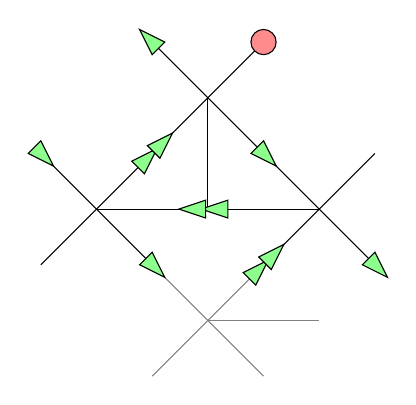
\begin{tikzpicture}
				
				\begin{scope}[xshift=0cm, rotate = -45]
					\begin{scope}[yshift = 2cm, rotate = -90]
						\vertex
						\begin{scope}[yshift = -1cm, xshift=0cm, rotate = -135]
							\biggreenarrow
						\end{scope}
					\end{scope}
					
					\begin{scope}[yshift = 2cm, xshift = 2cm, rotate = 180]
						\vertex
						\begin{scope}[xshift = 1cm, yshift=0cm, rotate = 135]
							\biggreenarrow
						\end{scope}
						\begin{scope}[xshift = -1cm, yshift=0cm, rotate = 135]
							\biggreenarrow
						\end{scope}
					\end{scope}
        				
					\vertex
						\begin{scope}[yshift = 3cm, rotate = 0]
							\fixededge
						\end{scope}
						\begin{scope}[xshift = -1cm, yshift=0cm, rotate = -45]
							\biggreenarrow
						\end{scope}
						\begin{scope}[xshift = 0cm, yshift=0.86cm, rotate = 45]
							\biggreenarrow
						\end{scope}
						\begin{scope}[xshift = 0cm, yshift=1.14cm, rotate = 45]
							\biggreenarrow
						\end{scope}

					\begin{scope}[xshift = 2cm, rotate = 0]
						\ghostvertex
						\begin{scope}[xshift = -1cm, yshift=0cm, rotate = -45]
							\biggreenarrow
						\end{scope}
						\begin{scope}[xshift = -0.9cm, yshift=1.1cm, rotate = 180]
							\biggreenarrow
						\end{scope}
						\begin{scope}[xshift = -1.1cm, yshift=0.9cm, rotate = 180]
							\biggreenarrow
						\end{scope}
						\begin{scope}[xshift = 0cm, yshift=0.86cm, rotate = 45]
							\biggreenarrow
						\end{scope}
						\begin{scope}[xshift = 0cm, yshift=1.14cm, rotate = 45]
							\biggreenarrow
						\end{scope}
						
					\end{scope}
				\end{scope}
								
				\end{tikzpicture}
				}
				}
				\caption{Next-to-next neighbour contractions with three interacting edges.}
				\label{fig:nnblock:3}
			\end{figure}
			
			\begin{figure}[!ht]
				\centering{
				\scalebox{0.6}{
				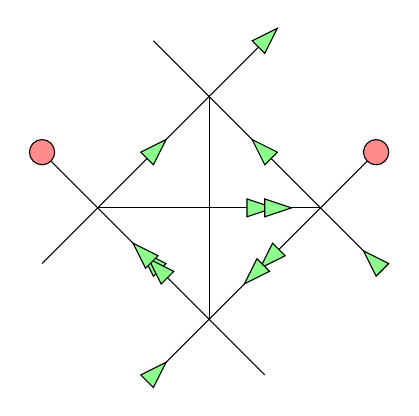
\begin{tikzpicture}
				
				\begin{scope}[xshift=0cm, rotate = 45]
					\begin{scope}[yshift = 2cm, rotate = -90]
						\vertex
						\begin{scope}[xshift = 1cm, yshift=0cm, rotate = 135]
							\biggreenarrow
						\end{scope}
					\end{scope}
					
					\begin{scope}[yshift = 2cm, xshift = 2cm, rotate = 180]
						\vertex
						\begin{scope}[xshift = 1cm, yshift=0cm, rotate = 135]
							\biggreenarrow
						\end{scope}
						\begin{scope}[xshift = -1cm, yshift=0cm, rotate = 135]
							\biggreenarrow
						\end{scope}
					\end{scope}
        				
					\vertex
						\begin{scope}[yshift = 3cm, rotate = 0]
							\fixededge
						\end{scope}
						\begin{scope}[xshift = -1cm, yshift=0cm, rotate = -45]
							\biggreenarrow
						\end{scope}
						\begin{scope}[xshift = 0cm, yshift=0.86cm, rotate = 45]
							\biggreenarrow
						\end{scope}
						\begin{scope}[xshift = 0cm, yshift=1.14cm, rotate = 45]
							\biggreenarrow
						\end{scope}

					\begin{scope}[xshift = 2cm, rotate = 90]
						\vertex
						\begin{scope}[yshift = -1cm, rotate = 90]
							\fixededge
						\end{scope}
						\begin{scope}[xshift = -1cm, yshift=0cm, rotate = -45]
							\biggreenarrow
						\end{scope}
						\begin{scope}[xshift = 1cm, yshift=0cm, rotate = -45]
							\biggreenarrow
						\end{scope}
						\begin{scope}[xshift = 0cm, yshift=0.86cm, rotate = 45]
							\biggreenarrow
						\end{scope}
						\begin{scope}[xshift = 0cm, yshift=1.14cm, rotate = 45]
							\biggreenarrow
						\end{scope}
						\begin{scope}[xshift = 0.58cm, yshift=0.58cm, rotate = 180]
							\biggreenarrow
						\end{scope}
						\begin{scope}[xshift = 0.42cm, yshift=0.42cm, rotate = 180]
							\biggreenarrow
						\end{scope}
					\end{scope}
				\end{scope}
								
				\end{tikzpicture}
				}
				}
				\caption{Next-to-next neighbour contractions with four interacting edges.}
				\label{fig:nnblock:4}
			\end{figure}
			
			
\subsection{Global modes}
\label{sec:modesvertex}

	Using the building blocks of Sec.\ref{sec:legovertex}, we can describe a few global modes.

				\begin{figure}[!ht]
				\centering{
				\scalebox{0.6}{
				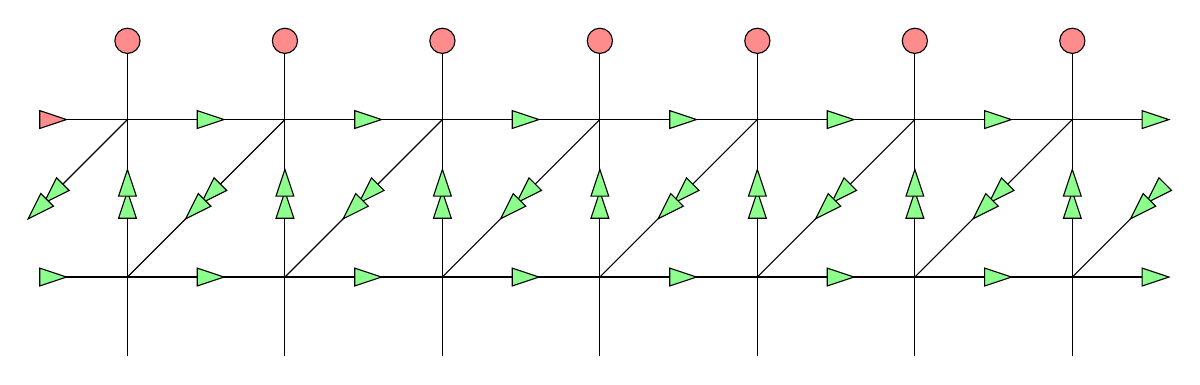
\begin{tikzpicture}
				
					\begin{scope}[yshift = 2cm, rotate = 180]
						\vertex
						\begin{scope}[xshift = 1cm, yshift=0cm, rotate = 135]
							\bigredarrow
						\end{scope}
					\end{scope}
					
					\begin{scope}[yshift = 2cm, xshift = 2cm, rotate = 180]
						\vertex
						\begin{scope}[xshift = 1cm, yshift=0cm, rotate = 135]
							\biggreenarrow
						\end{scope}
					\end{scope}
					
					\begin{scope}[yshift = 2cm, xshift = 4cm, rotate = 180]
						\vertex
						\begin{scope}[xshift = 1cm, yshift=0cm, rotate = 135]
							\biggreenarrow
						\end{scope}
					\end{scope}

					\begin{scope}[yshift = 2cm, xshift = 6cm, rotate = 180]
						\vertex
						\begin{scope}[xshift = 1cm, yshift=0cm, rotate = 135]
							\biggreenarrow
						\end{scope}
					\end{scope}

					\begin{scope}[yshift = 2cm, xshift = 8cm, rotate = 180]
						\vertex
						\begin{scope}[xshift = 1cm, yshift=0cm, rotate = 135]
							\biggreenarrow
						\end{scope}
					\end{scope}
					
					\begin{scope}[yshift = 2cm, xshift = 10cm, rotate = 180]
						\vertex
						\begin{scope}[xshift = 1cm, yshift=0cm, rotate = 135]
							\biggreenarrow
						\end{scope}
					\end{scope}
					
					\begin{scope}[yshift = 2cm, xshift = 12cm, rotate = 180]
						\vertex
						\begin{scope}[xshift = 1cm, yshift=0cm, rotate = 135]
							\biggreenarrow
						\end{scope}
						\begin{scope}[xshift = -1cm, yshift=0cm, rotate = 135]
							\biggreenarrow
						\end{scope}
					\end{scope}
        				
					\vertex
						\begin{scope}[yshift = 3cm, rotate = 0]
							\fixededge
						\end{scope}
						\begin{scope}[xshift = -1cm, yshift=0cm, rotate = -45]
							\biggreenarrow
						\end{scope}
						\begin{scope}[xshift = -0.9cm, yshift=1.1cm, rotate = 180]
							\biggreenarrow
						\end{scope}
						\begin{scope}[xshift = -1.1cm, yshift=0.9cm, rotate = 180]
							\biggreenarrow
						\end{scope}
						\begin{scope}[xshift = 0cm, yshift=0.86cm, rotate = 45]
							\biggreenarrow
						\end{scope}
						\begin{scope}[xshift = 0cm, yshift=1.14cm, rotate = 45]
							\biggreenarrow
						\end{scope}

					\begin{scope}[xshift = 2cm, rotate = 0]
						\vertex
						\begin{scope}[yshift = 3cm, rotate = 0]
							\fixededge
						\end{scope}
						\begin{scope}[xshift = -1cm, yshift=0cm, rotate = -45]
							\biggreenarrow
						\end{scope}
						\begin{scope}[xshift = -0.9cm, yshift=1.1cm, rotate = 180]
							\biggreenarrow
						\end{scope}
						\begin{scope}[xshift = -1.1cm, yshift=0.9cm, rotate = 180]
							\biggreenarrow
						\end{scope}
						\begin{scope}[xshift = 0cm, yshift=0.86cm, rotate = 45]
							\biggreenarrow
						\end{scope}
						\begin{scope}[xshift = 0cm, yshift=1.14cm, rotate = 45]
							\biggreenarrow
						\end{scope}
					\end{scope}
					
					\begin{scope}[xshift = 4cm, rotate = 0]
						\vertex
						\begin{scope}[yshift = 3cm, rotate = 0]
							\fixededge
						\end{scope}
						\begin{scope}[xshift = -1cm, yshift=0cm, rotate = -45]
							\biggreenarrow
						\end{scope}
						\begin{scope}[xshift = -0.9cm, yshift=1.1cm, rotate = 180]
							\biggreenarrow
						\end{scope}
						\begin{scope}[xshift = -1.1cm, yshift=0.9cm, rotate = 180]
							\biggreenarrow
						\end{scope}
						\begin{scope}[xshift = 0cm, yshift=0.86cm, rotate = 45]
							\biggreenarrow
						\end{scope}
						\begin{scope}[xshift = 0cm, yshift=1.14cm, rotate = 45]
							\biggreenarrow
						\end{scope}
					\end{scope}

					\begin{scope}[xshift = 6cm, rotate = 0]
						\vertex
						\begin{scope}[yshift = 3cm, rotate = 0]
							\fixededge
						\end{scope}
						\begin{scope}[xshift = -1cm, yshift=0cm, rotate = -45]
							\biggreenarrow
						\end{scope}
						\begin{scope}[xshift = -0.9cm, yshift=1.1cm, rotate = 180]
							\biggreenarrow
						\end{scope}
						\begin{scope}[xshift = -1.1cm, yshift=0.9cm, rotate = 180]
							\biggreenarrow
						\end{scope}
						\begin{scope}[xshift = 0cm, yshift=0.86cm, rotate = 45]
							\biggreenarrow
						\end{scope}
						\begin{scope}[xshift = 0cm, yshift=1.14cm, rotate = 45]
							\biggreenarrow
						\end{scope}
					\end{scope}

					\begin{scope}[xshift = 8cm, rotate = 0]
						\vertex
						\begin{scope}[yshift = 3cm, rotate = 0]
							\fixededge
						\end{scope}
						\begin{scope}[xshift = -1cm, yshift=0cm, rotate = -45]
							\biggreenarrow
						\end{scope}
						\begin{scope}[xshift = -0.9cm, yshift=1.1cm, rotate = 180]
							\biggreenarrow
						\end{scope}
						\begin{scope}[xshift = -1.1cm, yshift=0.9cm, rotate = 180]
							\biggreenarrow
						\end{scope}
						\begin{scope}[xshift = 0cm, yshift=0.86cm, rotate = 45]
							\biggreenarrow
						\end{scope}
						\begin{scope}[xshift = 0cm, yshift=1.14cm, rotate = 45]
							\biggreenarrow
						\end{scope}
					\end{scope}
					
					\begin{scope}[xshift = 10cm, rotate = 0]
						\vertex
						\begin{scope}[yshift = 3cm, rotate = 0]
							\fixededge
						\end{scope}
						\begin{scope}[xshift = -1cm, yshift=0cm, rotate = -45]
							\biggreenarrow
						\end{scope}
						\begin{scope}[xshift = -0.9cm, yshift=1.1cm, rotate = 180]
							\biggreenarrow
						\end{scope}
						\begin{scope}[xshift = -1.1cm, yshift=0.9cm, rotate = 180]
							\biggreenarrow
						\end{scope}
						\begin{scope}[xshift = 0cm, yshift=0.86cm, rotate = 45]
							\biggreenarrow
						\end{scope}
						\begin{scope}[xshift = 0cm, yshift=1.14cm, rotate = 45]
							\biggreenarrow
						\end{scope}
					\end{scope}
					
					\begin{scope}[xshift = 12cm, rotate = 0]
						\vertex
						\begin{scope}[yshift = 3cm, rotate = 0]
							\fixededge
						\end{scope}
						\begin{scope}[xshift = -1cm, yshift=0cm, rotate = -45]
							\biggreenarrow
						\end{scope}
						\begin{scope}[xshift = 1cm, yshift=0cm, rotate = -45]
							\biggreenarrow
						\end{scope}
						\begin{scope}[xshift = -0.9cm, yshift=1.1cm, rotate = 180]
							\biggreenarrow
						\end{scope}
						\begin{scope}[xshift = -1.1cm, yshift=0.9cm, rotate = 180]
							\biggreenarrow
						\end{scope}
						\begin{scope}[xshift = 1.1cm, yshift=1.1cm, rotate = 180]
							\biggreenarrow
						\end{scope}
						\begin{scope}[xshift = 0.9cm, yshift=0.9cm, rotate = 180]
							\biggreenarrow
						\end{scope}
						\begin{scope}[xshift = 0cm, yshift=0.86cm, rotate = 45]
							\biggreenarrow
						\end{scope}
						\begin{scope}[xshift = 0cm, yshift=1.14cm, rotate = 45]
							\biggreenarrow
						\end{scope}
					\end{scope}
								
				\end{tikzpicture}
				}
				}
				\caption{Vertex configuration of an activated bump mechanism. The red points/arrows denote fixed angles, while the green ones are constrained by the former.}
				\label{fig:bump}
			\end{figure}
			
			\begin{figure}[!ht]
				\centering{
				\scalebox{0.6}{
				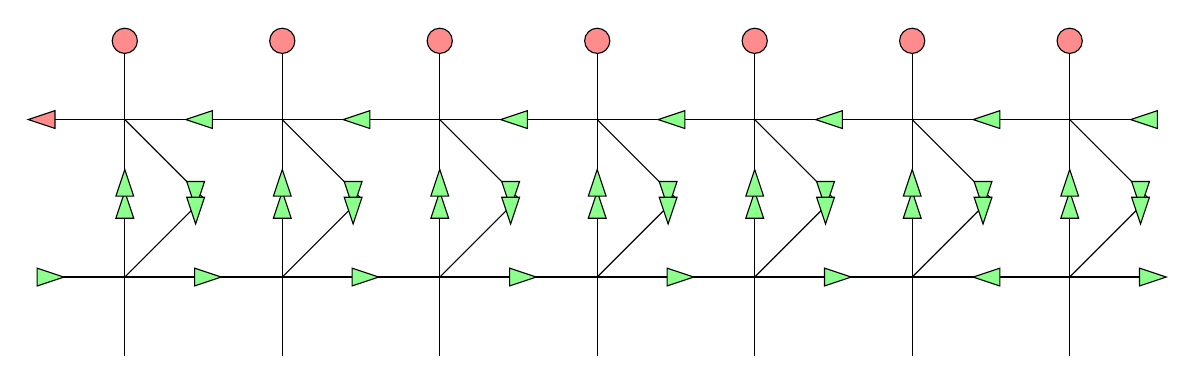
\begin{tikzpicture}
				
					\begin{scope}[yshift = 2cm, rotate = 270]
						\vertex
						\begin{scope}[xshift = 0cm, yshift=-1cm, rotate = -135]
							\bigredarrow
						\end{scope}
					\end{scope}
					
					\begin{scope}[yshift = 2cm, xshift = 2cm, rotate = 270]
						\vertex
						\begin{scope}[xshift = 0cm, yshift=-1cm, rotate = -135]
							\biggreenarrow
						\end{scope}
					\end{scope}
					
					\begin{scope}[yshift = 2cm, xshift = 4cm, rotate = 270]
						\vertex
						\begin{scope}[xshift = 0cm, yshift=-1cm, rotate = -135]
							\biggreenarrow
						\end{scope}
					\end{scope}

					\begin{scope}[yshift = 2cm, xshift = 6cm, rotate = 270]
						\vertex
						\begin{scope}[xshift = 0cm, yshift=-1cm, rotate = -135]
							\biggreenarrow
						\end{scope}
					\end{scope}

					\begin{scope}[yshift = 2cm, xshift = 8cm, rotate = 270]
						\vertex
						\begin{scope}[xshift = 0cm, yshift=-1cm, rotate = -135]
							\biggreenarrow
						\end{scope}
					\end{scope}
					
					\begin{scope}[yshift = 2cm, xshift = 10cm, rotate = 270]
						\vertex
						\begin{scope}[xshift = 0cm, yshift=-1cm, rotate = -135]
							\biggreenarrow
						\end{scope}
					\end{scope}
					
					\begin{scope}[yshift = 2cm, xshift = 12cm, rotate = 270]
						\vertex
						\begin{scope}[xshift = 0cm, yshift=-1cm, rotate = -135]
							\biggreenarrow
						\end{scope}
						\begin{scope}[xshift = 0cm, yshift=1cm, rotate = -135]
							\biggreenarrow
						\end{scope}
					\end{scope}
        				
					\vertex
						\begin{scope}[yshift = 3cm, rotate = 0]
							\fixededge
						\end{scope}
						\begin{scope}[yshift = 0.86cm, rotate = 45]
							\biggreenarrow
						\end{scope}
						\begin{scope}[yshift = 1.14cm, rotate = 45]
							\biggreenarrow
						\end{scope}
						\begin{scope}[xshift=0.9cm,yshift = 1.1cm, rotate = -135]
							\biggreenarrow
						\end{scope}
						\begin{scope}[xshift=0.9cm,yshift = 0.9cm, rotate = -135]
							\biggreenarrow
						\end{scope}
						\begin{scope}[xshift = -1cm, yshift=0cm, rotate = -45]
							\biggreenarrow
						\end{scope}

					\begin{scope}[xshift = 2cm, rotate = 0]
						\vertex
						\begin{scope}[yshift = 3cm, rotate = 0]
							\fixededge
						\end{scope}
						\begin{scope}[yshift = 0.86cm, rotate = 45]
							\biggreenarrow
						\end{scope}
						\begin{scope}[yshift = 1.14cm, rotate = 45]
							\biggreenarrow
						\end{scope}
						\begin{scope}[xshift=0.9cm,yshift = 1.1cm, rotate = -135]
							\biggreenarrow
						\end{scope}
						\begin{scope}[xshift=0.9cm,yshift = 0.9cm, rotate = -135]
							\biggreenarrow
						\end{scope}
						\begin{scope}[xshift = -1cm, yshift=0cm, rotate = -45]
							\biggreenarrow
						\end{scope}
					\end{scope}
					
					\begin{scope}[xshift = 4cm, rotate = 0]
						\vertex
						\begin{scope}[yshift = 3cm, rotate = 0]
							\fixededge
						\end{scope}
						\begin{scope}[yshift = 0.86cm, rotate = 45]
							\biggreenarrow
						\end{scope}
						\begin{scope}[yshift = 1.14cm, rotate = 45]
							\biggreenarrow
						\end{scope}
						\begin{scope}[xshift=0.9cm,yshift = 1.1cm, rotate = -135]
							\biggreenarrow
						\end{scope}
						\begin{scope}[xshift=0.9cm,yshift = 0.9cm, rotate = -135]
							\biggreenarrow
						\end{scope}
						\begin{scope}[xshift = -1cm, yshift=0cm, rotate = -45]
							\biggreenarrow
						\end{scope}
					\end{scope}

					\begin{scope}[xshift = 6cm, rotate = 0]
						\vertex
						\begin{scope}[yshift = 3cm, rotate = 0]
							\fixededge
						\end{scope}
						\begin{scope}[yshift = 0.86cm, rotate = 45]
							\biggreenarrow
						\end{scope}
						\begin{scope}[yshift = 1.14cm, rotate = 45]
							\biggreenarrow
						\end{scope}
						\begin{scope}[xshift=0.9cm,yshift = 1.1cm, rotate = -135]
							\biggreenarrow
						\end{scope}
						\begin{scope}[xshift=0.9cm,yshift = 0.9cm, rotate = -135]
							\biggreenarrow
						\end{scope}
						\begin{scope}[xshift = -1cm, yshift=0cm, rotate = -45]
							\biggreenarrow
						\end{scope}
					\end{scope}

					\begin{scope}[xshift = 8cm, rotate = 0]
						\vertex
						\begin{scope}[yshift = 3cm, rotate = 0]
							\fixededge
						\end{scope}
						\begin{scope}[yshift = 0.86cm, rotate = 45]
							\biggreenarrow
						\end{scope}
						\begin{scope}[yshift = 1.14cm, rotate = 45]
							\biggreenarrow
						\end{scope}
						\begin{scope}[xshift=0.9cm,yshift = 1.1cm, rotate = -135]
							\biggreenarrow
						\end{scope}
						\begin{scope}[xshift=0.9cm,yshift = 0.9cm, rotate = -135]
							\biggreenarrow
						\end{scope}
						\begin{scope}[xshift = -1cm, yshift=0cm, rotate = -45]
							\biggreenarrow
						\end{scope}
					\end{scope}
					
					\begin{scope}[xshift = 10cm, rotate = 0]
						\vertex
						\begin{scope}[yshift = 3cm, rotate = 0]
							\fixededge
						\end{scope}
						\begin{scope}[yshift = 0.86cm, rotate = 45]
							\biggreenarrow
						\end{scope}
						\begin{scope}[yshift = 1.14cm, rotate = 45]
							\biggreenarrow
						\end{scope}
						\begin{scope}[xshift=0.9cm,yshift = 1.1cm, rotate = -135]
							\biggreenarrow
						\end{scope}
						\begin{scope}[xshift=0.9cm,yshift = 0.9cm, rotate = -135]
							\biggreenarrow
						\end{scope}
						\begin{scope}[xshift = -1cm, yshift=0cm, rotate = -45]
							\biggreenarrow
						\end{scope}
					\end{scope}
					
					\begin{scope}[xshift = 12cm, rotate = 0]
						\vertex
						\begin{scope}[yshift = 3cm, rotate = 0]
							\fixededge
						\end{scope}
						\begin{scope}[yshift = 0.86cm, rotate = 45]
							\biggreenarrow
						\end{scope}
						\begin{scope}[yshift = 1.14cm, rotate = 45]
							\biggreenarrow
						\end{scope}
						\begin{scope}[xshift=0.9cm,yshift = 1.1cm, rotate = -135]
							\biggreenarrow
						\end{scope}
						\begin{scope}[xshift=0.9cm,yshift = 0.9cm, rotate = -135]
							\biggreenarrow
						\end{scope}
						\begin{scope}[xshift = -1cm, yshift=0cm, rotate = 135]
							\biggreenarrow
						\end{scope}
						\begin{scope}[xshift = 1cm, yshift=0cm, rotate = -45]
							\biggreenarrow
						\end{scope}
					\end{scope}
								
				\end{tikzpicture}
				}
				}
				\caption{Vertex configuration of an activated antibump mechanism. The red points/arrows denote fixed angles, while the green ones are constrained by the former.}
				\label{fig:antibump}
			\end{figure}
			
			\begin{figure}[!ht]
				\centering{
				\scalebox{0.6}{
				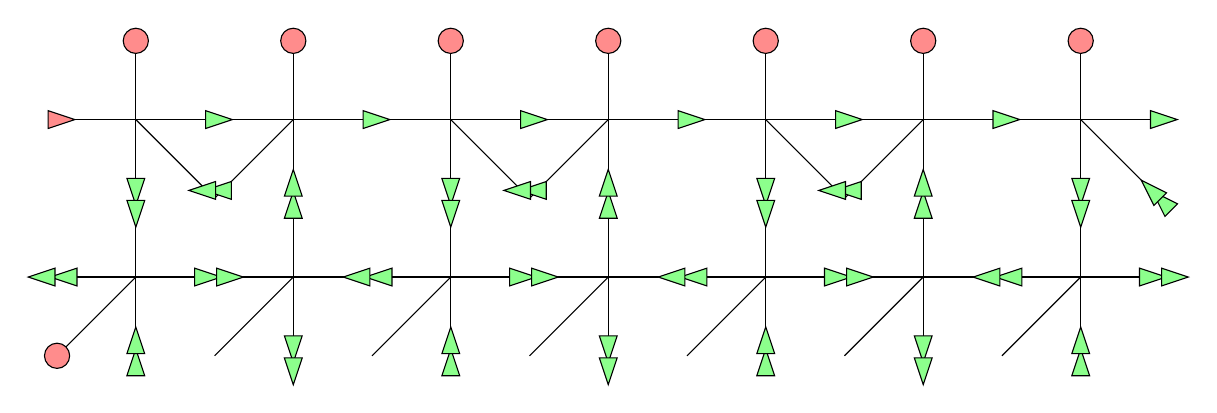
\begin{tikzpicture}
				
					\begin{scope}[yshift = 2cm, rotate = 270]
						\vertex
						\begin{scope}[xshift = 0cm, yshift=-1cm, rotate = 45]
							\bigredarrow
						\end{scope}
					\end{scope}
					
					\begin{scope}[yshift = 2cm, xshift = 2cm, rotate = 180]
						\vertex
						\begin{scope}[xshift = 1cm, yshift=0cm, rotate = 135]
							\biggreenarrow
						\end{scope}
						\begin{scope}[xshift = 0.9cm, yshift=0.9cm, rotate = -45]
							\biggreenarrow
						\end{scope}
						\begin{scope}[xshift = 1.1cm, yshift=0.9cm, rotate = -45]
							\biggreenarrow
						\end{scope}
					\end{scope}
					
					\begin{scope}[yshift = 2cm, xshift = 4cm, rotate = 270]
						\vertex
						\begin{scope}[xshift = 0cm, yshift=-1cm, rotate = 45]
							\biggreenarrow
						\end{scope}
					\end{scope}

					\begin{scope}[yshift = 2cm, xshift = 6cm, rotate = 180]
						\vertex
						\begin{scope}[xshift = 1cm, yshift=0cm, rotate = 135]
							\biggreenarrow
						\end{scope}
						\begin{scope}[xshift = 0.9cm, yshift=0.9cm, rotate = -45]
							\biggreenarrow
						\end{scope}
						\begin{scope}[xshift = 1.1cm, yshift=0.9cm, rotate = -45]
							\biggreenarrow
						\end{scope}
					\end{scope}

					\begin{scope}[yshift = 2cm, xshift = 8cm, rotate = 270]
						\vertex
						\begin{scope}[xshift = 0cm, yshift=-1cm, rotate = 45]
							\biggreenarrow
						\end{scope}
					\end{scope}
					
					\begin{scope}[yshift = 2cm, xshift = 10cm, rotate = 180]
						\vertex
						\begin{scope}[xshift = 1cm, yshift=0cm, rotate = 135]
							\biggreenarrow
						\end{scope}
						\begin{scope}[xshift = 0.9cm, yshift=0.9cm, rotate = -45]
							\biggreenarrow
						\end{scope}
						\begin{scope}[xshift = 1.1cm, yshift=0.9cm, rotate = -45]
							\biggreenarrow
						\end{scope}
					\end{scope}
					
					\begin{scope}[yshift = 2cm, xshift = 12cm, rotate = 270]
						\vertex
						\begin{scope}[xshift = 0cm, yshift=-1cm, rotate = 45]
							\biggreenarrow
						\end{scope}
						\begin{scope}[xshift = 0cm, yshift=1cm, rotate = 45]
							\biggreenarrow
						\end{scope}
						\begin{scope}[xshift = 1.07cm, yshift=1.07cm, rotate = -180]
							\biggreenarrow
						\end{scope}
						\begin{scope}[xshift = 0.93cm, yshift=0.93cm, rotate = -180]
							\biggreenarrow
						\end{scope}
					\end{scope}
        				
        			\begin{scope}[xshift = 0cm, rotate = 180]
						\vertex
						\begin{scope}[yshift = -3cm, rotate = 180]
							\fixededge
						\end{scope}
						\begin{scope}[xshift = 1cm, yshift = 1cm, rotate = 0]
							\fixededge
						\end{scope}
						\begin{scope}[yshift = -1.14cm, rotate = 45]
							\biggreenarrow
						\end{scope}
						\begin{scope}[yshift = -0.86cm, rotate = 45]
							\biggreenarrow
						\end{scope}
						\begin{scope}[yshift = 1.14cm, rotate = -135]
							\biggreenarrow
						\end{scope}
						\begin{scope}[yshift = 0.86cm, rotate = -135]
							\biggreenarrow
						\end{scope}
						\begin{scope}[xshift = 0.86cm, yshift=0cm, rotate = -45]
							\biggreenarrow
						\end{scope}
						\begin{scope}[xshift = 1.14cm, yshift=0cm, rotate = -45]
							\biggreenarrow
						\end{scope}
					\end{scope}


					\begin{scope}[xshift = 2cm, rotate = 180]
						\vertex
						\begin{scope}[yshift = -3cm, rotate = 180]
							\fixededge
						\end{scope}
						\begin{scope}[yshift = -0.86cm, rotate = -135]
							\biggreenarrow
						\end{scope}
						\begin{scope}[yshift = -1.14cm, rotate = -135]
							\biggreenarrow
						\end{scope}
						\begin{scope}[yshift = 0.86cm, rotate = 45]
							\biggreenarrow
						\end{scope}
						\begin{scope}[yshift = 1.14cm, rotate = 45]
							\biggreenarrow
						\end{scope}
						\begin{scope}[xshift = 1.14cm, yshift=0cm, rotate = 135]
							\biggreenarrow
						\end{scope}
						\begin{scope}[xshift = 0.86cm, yshift=0cm, rotate = 135]
							\biggreenarrow
						\end{scope}
					\end{scope}
					
					\begin{scope}[xshift = 4cm, rotate = 180]
						\vertex
						\begin{scope}[yshift = -3cm, rotate = 180]
							\fixededge
						\end{scope}
						\begin{scope}[yshift = -1.14cm, rotate = 45]
							\biggreenarrow
						\end{scope}
						\begin{scope}[yshift = -0.86cm, rotate = 45]
							\biggreenarrow
						\end{scope}
						\begin{scope}[yshift = 1.14cm, rotate = -135]
							\biggreenarrow
						\end{scope}
						\begin{scope}[yshift = 0.86cm, rotate = -135]
							\biggreenarrow
						\end{scope}
						\begin{scope}[xshift = 0.86cm, yshift=0cm, rotate = -45]
							\biggreenarrow
						\end{scope}
						\begin{scope}[xshift = 1.14cm, yshift=0cm, rotate = -45]
							\biggreenarrow
						\end{scope}
					\end{scope}

					\begin{scope}[xshift = 6cm, rotate = 180]
						\vertex
						\begin{scope}[yshift = -3cm, rotate = 180]
							\fixededge
						\end{scope}
						\begin{scope}[yshift = -0.86cm, rotate = -135]
							\biggreenarrow
						\end{scope}
						\begin{scope}[yshift = -1.14cm, rotate = -135]
							\biggreenarrow
						\end{scope}
						\begin{scope}[yshift = 0.86cm, rotate = 45]
							\biggreenarrow
						\end{scope}
						\begin{scope}[yshift = 1.14cm, rotate = 45]
							\biggreenarrow
						\end{scope}
						\begin{scope}[xshift = 1.14cm, yshift=0cm, rotate = 135]
							\biggreenarrow
						\end{scope}
						\begin{scope}[xshift = 0.86cm, yshift=0cm, rotate = 135]
							\biggreenarrow
						\end{scope}
					\end{scope}

					\begin{scope}[xshift = 8cm, rotate = 180]
						\vertex
						\begin{scope}[yshift = -3cm, rotate = 180]
							\fixededge
						\end{scope}
						\begin{scope}[yshift = -1.14cm, rotate = 45]
							\biggreenarrow
						\end{scope}
						\begin{scope}[yshift = -0.86cm, rotate = 45]
							\biggreenarrow
						\end{scope}
						\begin{scope}[yshift = 1.14cm, rotate = -135]
							\biggreenarrow
						\end{scope}
						\begin{scope}[yshift = 0.86cm, rotate = -135]
							\biggreenarrow
						\end{scope}
						\begin{scope}[xshift = 0.86cm, yshift=0cm, rotate = -45]
							\biggreenarrow
						\end{scope}
						\begin{scope}[xshift = 1.14cm, yshift=0cm, rotate = -45]
							\biggreenarrow
						\end{scope}
					\end{scope}
					
					\begin{scope}[xshift = 10cm, rotate = 180]
						\vertex
						\begin{scope}[yshift = -3cm, rotate = 180]
							\fixededge
						\end{scope}
						\begin{scope}[yshift = -0.86cm, rotate = -135]
							\biggreenarrow
						\end{scope}
						\begin{scope}[yshift = -1.14cm, rotate = -135]
							\biggreenarrow
						\end{scope}
						\begin{scope}[yshift = 0.86cm, rotate = 45]
							\biggreenarrow
						\end{scope}
						\begin{scope}[yshift = 1.14cm, rotate = 45]
							\biggreenarrow
						\end{scope}
						\begin{scope}[xshift = 1.14cm, yshift=0cm, rotate = 135]
							\biggreenarrow
						\end{scope}
						\begin{scope}[xshift = 0.86cm, yshift=0cm, rotate = 135]
							\biggreenarrow
						\end{scope}
					\end{scope}
					
					\begin{scope}[xshift = 12cm, rotate = 180]
						\vertex
						\begin{scope}[yshift = -3cm, rotate = 180]
							\fixededge
						\end{scope}
						\begin{scope}[yshift = -1.14cm, rotate = 45]
							\biggreenarrow
						\end{scope}
						\begin{scope}[yshift = -0.86cm, rotate = 45]
							\biggreenarrow
						\end{scope}
						\begin{scope}[yshift = 1.14cm, rotate = -135]
							\biggreenarrow
						\end{scope}
						\begin{scope}[yshift = 0.86cm, rotate = -135]
							\biggreenarrow
						\end{scope}
						\begin{scope}[xshift = 0.86cm, yshift=0cm, rotate = -45]
							\biggreenarrow
						\end{scope}
						\begin{scope}[xshift = 1.14cm, yshift=0cm, rotate = -45]
							\biggreenarrow
						\end{scope}
						\begin{scope}[xshift = -0.86cm, yshift=0cm, rotate = 135]
							\biggreenarrow
						\end{scope}
						\begin{scope}[xshift = -1.14cm, yshift=0cm, rotate = 135]
							\biggreenarrow
						\end{scope}
					\end{scope}
								
				\end{tikzpicture}
				}
				}
				\caption{Vertex configuration of an activated "domain wall" mechanism. The red points denote fixed angles.}
				\label{fig:domainwall}
			\end{figure}
			
							\begin{figure}[!ht]
				\centering{
				\scalebox{0.6}{
				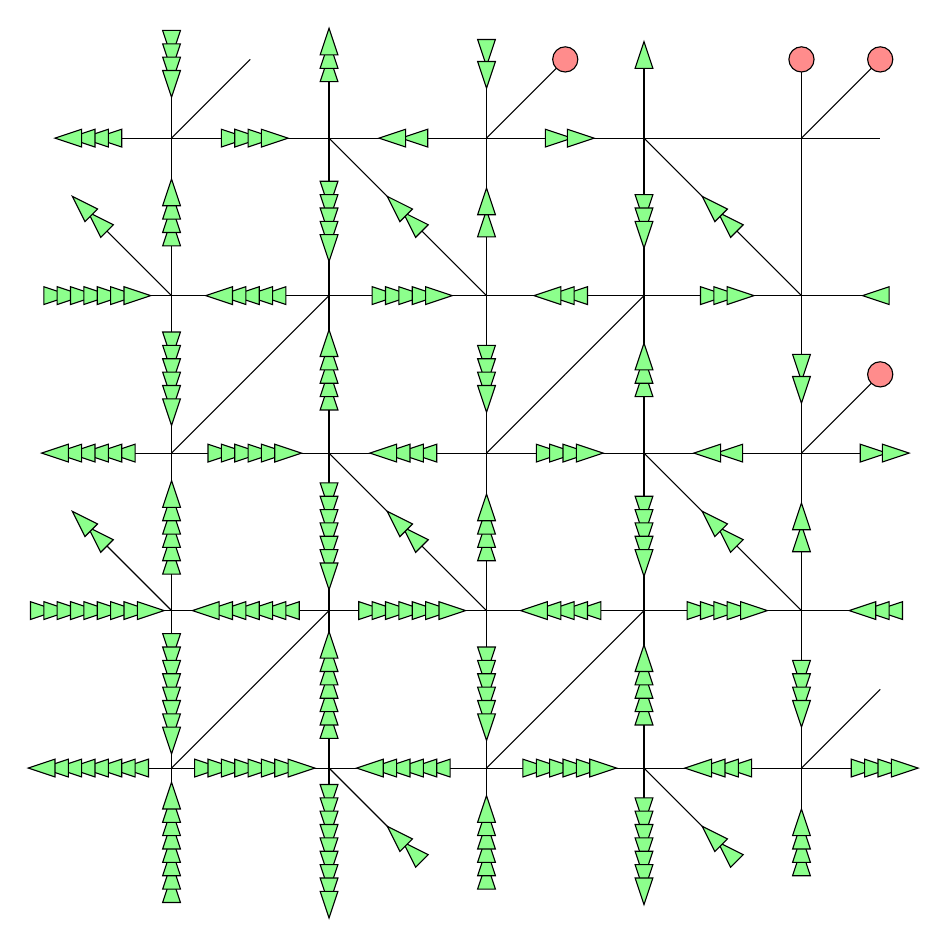
\begin{tikzpicture}
        				
					\vertex
					\begin{scope}[yshift = -1cm, rotate = 45]
							\octuplegreenarrow
						\end{scope}
						\begin{scope}[xshift = -1cm, yshift=0cm, rotate = 135]
							\octuplegreenarrow
						\end{scope}

					\begin{scope}[xshift = 2cm, rotate = 270]
						\vertex
						\begin{scope}[yshift = -1cm, rotate = 45]
							\octuplegreenarrow
						\end{scope}
						\begin{scope}[xshift = 1cm, yshift=0cm, rotate = -45]
							\enneatuplegreenarrow
						\end{scope}
						\begin{scope}[xshift = 1.1cm, yshift=1.1cm, rotate = 180]
							\biggreenarrow
						\end{scope}
						\begin{scope}[xshift = 0.9cm, yshift=0.9cm, rotate = 180]
							\biggreenarrow
						\end{scope}
					\end{scope}
					
					\begin{scope}[xshift = 4cm, rotate = 0]
						\vertex
						\begin{scope}[yshift = -1cm, rotate = 45]
							\sextuplegreenarrow
						\end{scope}
						\begin{scope}[xshift = -1cm, yshift=0cm, rotate = 135]
							\sextuplegreenarrow
						\end{scope}
					\end{scope}

					\begin{scope}[xshift = 6cm, rotate = 270]
						\vertex
						\begin{scope}[yshift = -1cm, rotate = 45]
							\sextuplegreenarrow
						\end{scope}
						\begin{scope}[xshift = 1cm, yshift=0cm, rotate = -45]
							\heptuplegreenarrow
						\end{scope}
						\begin{scope}[xshift = 1.1cm, yshift=1.1cm, rotate = 180]
							\biggreenarrow
						\end{scope}
						\begin{scope}[xshift = 0.9cm, yshift=0.9cm, rotate = 180]
							\biggreenarrow
						\end{scope}
					\end{scope}

					\begin{scope}[xshift = 8cm, rotate = 0]
						\vertex
						\begin{scope}[yshift = -1cm, rotate = 45]
							\quadruplegreenarrow
						\end{scope}
						\begin{scope}[xshift = -1cm, yshift=0cm, rotate = 135]
							\quadruplegreenarrow
						\end{scope}
						\begin{scope}[xshift = 1cm, yshift=0cm, rotate = -45]
							\quadruplegreenarrow
						\end{scope}
					\end{scope}
					
					\begin{scope}[yshift = 2cm, rotate = 90]
						\vertex
						\begin{scope}[xshift = -1cm, yshift=0cm, rotate = 135]
							\octuplegreenarrow
						\end{scope}
						\begin{scope}[yshift = 1cm, rotate = -135]
							\enneatuplegreenarrow
						\end{scope}
						\begin{scope}[xshift = 0.9cm, yshift=0.9cm, rotate = 0]
							\biggreenarrow
						\end{scope}
						\begin{scope}[xshift = 1.1cm, yshift=1.1cm, rotate = 0]
							\biggreenarrow
						\end{scope}
					\end{scope}
					
					\begin{scope}[yshift = 2cm, xshift = 2cm, rotate = 180]
						\vertex
						\begin{scope}[yshift = 1cm, rotate = -135]
							\heptuplegreenarrow
						\end{scope}
						\begin{scope}[xshift = 1cm, yshift=0cm, rotate = -45]
							\heptuplegreenarrow
						\end{scope}
					\end{scope}
					
					\begin{scope}[yshift = 2cm, xshift = 4cm, rotate = 90]
						\vertex
						\begin{scope}[xshift = -1cm, yshift=0cm, rotate = 135]
							\sextuplegreenarrow
						\end{scope}
						\begin{scope}[yshift = 1cm, rotate = -135]
							\heptuplegreenarrow
						\end{scope}
					\end{scope}

					\begin{scope}[yshift = 2cm, xshift = 6cm, rotate = 180]
						\vertex
						\begin{scope}[yshift = 1cm, rotate = -135]
							\quintuplegreenarrow
						\end{scope}
						\begin{scope}[xshift = 1cm, yshift=0cm, rotate = -45]
							\quintuplegreenarrow
						\end{scope}
					\end{scope}

					\begin{scope}[yshift = 2cm, xshift = 8cm, rotate = 90]
						\vertex
						\begin{scope}[yshift = -1cm, rotate = 45]
							\triplegreenarrow
						\end{scope}
						\begin{scope}[xshift = -1cm, yshift=0cm, rotate = 135]
							\quadruplegreenarrow
						\end{scope}
						\begin{scope}[yshift = 1cm, rotate = -135]
							\quintuplegreenarrow
						\end{scope}
					\end{scope}
					
					\begin{scope}[yshift = 4cm, rotate = 0]
						\vertex
						\begin{scope}[yshift = -1cm, rotate = 45]
							\sextuplegreenarrow
						\end{scope}
						\begin{scope}[xshift = -1cm, yshift=0cm, rotate = 135]
							\sextuplegreenarrow
						\end{scope}
					\end{scope}
					
					\begin{scope}[yshift = 4cm, xshift = 2cm, rotate = 270]
						\vertex
						\begin{scope}[yshift = -1cm, rotate = 45]
							\sextuplegreenarrow
						\end{scope}
						\begin{scope}[xshift = 1cm, yshift=0cm, rotate = -45]
							\heptuplegreenarrow
						\end{scope}
						\begin{scope}[xshift = 1.1cm, yshift=1.1cm, rotate = 180]
							\biggreenarrow
						\end{scope}
						\begin{scope}[xshift = 0.9cm, yshift=0.9cm, rotate = 180]
							\biggreenarrow
						\end{scope}
					\end{scope}
					
					\begin{scope}[yshift = 4cm, xshift = 4cm, rotate = 0]
						\vertex
						\begin{scope}[yshift = -1cm, rotate = 45]
							\quadruplegreenarrow
						\end{scope}
						\begin{scope}[xshift = -1cm, yshift=0cm, rotate = 135]
							\quadruplegreenarrow
						\end{scope}
					\end{scope}

					\begin{scope}[yshift = 4cm, xshift = 6cm, rotate = 270]
						\vertex
						\begin{scope}[yshift = -1cm, rotate = 45]
							\quadruplegreenarrow
						\end{scope}
						\begin{scope}[xshift = 1cm, yshift=0cm, rotate = -45]
							\quintuplegreenarrow
						\end{scope}
						\begin{scope}[xshift = 1.1cm, yshift=1.1cm, rotate = 180]
							\biggreenarrow
						\end{scope}
						\begin{scope}[xshift = 0.9cm, yshift=0.9cm, rotate = 180]
							\biggreenarrow
						\end{scope}
					\end{scope}

					\begin{scope}[yshift = 4cm, xshift = 8cm, rotate = 0]
						\vertex
						\begin{scope}[yshift = 1cm, xshift = 1cm]
							\fixededge
						\end{scope}
						\begin{scope}[yshift = -1.14cm, rotate = 45]
							\biggreenarrow
						\end{scope}
						\begin{scope}[yshift = -0.86cm, rotate = 45]
							\biggreenarrow
						\end{scope}
						\begin{scope}[xshift = -0.86cm, yshift=0cm, rotate = 135]
							\biggreenarrow
						\end{scope}
						\begin{scope}[xshift = -1.14cm, yshift=0cm, rotate = 135]
							\biggreenarrow
						\end{scope}
						\begin{scope}[xshift = 0.86cm, yshift=0cm, rotate = -45]
							\biggreenarrow
						\end{scope}
						\begin{scope}[xshift = 1.14cm, yshift=0cm, rotate = -45]
							\biggreenarrow
						\end{scope}
					\end{scope}
					
					\begin{scope}[yshift = 6cm, rotate = 90]
						\vertex
						\begin{scope}[xshift = -1cm, yshift=0cm, rotate = 135]
							\sextuplegreenarrow
						\end{scope}
						\begin{scope}[yshift = 1cm, rotate = -135]
							\heptuplegreenarrow
						\end{scope}
						\begin{scope}[xshift = 0.9cm, yshift=0.9cm, rotate = 0]
							\biggreenarrow
						\end{scope}
						\begin{scope}[xshift = 1.1cm, yshift=1.1cm, rotate = 0]
							\biggreenarrow
						\end{scope}
					\end{scope}
					
					\begin{scope}[yshift = 6cm, xshift = 2cm, rotate = 180]
						\vertex
						\begin{scope}[yshift = 1cm, rotate = -135]
							\quintuplegreenarrow
						\end{scope}
						\begin{scope}[xshift = 1cm, yshift=0cm, rotate = -45]
							\quintuplegreenarrow
						\end{scope}
					\end{scope}
					
					\begin{scope}[yshift = 6cm, xshift = 4cm, rotate = 90]
						\vertex
						\begin{scope}[xshift = -1cm, yshift=0cm, rotate = 135]
							\quadruplegreenarrow
						\end{scope}
						\begin{scope}[yshift = 1cm, rotate = -135]
							\quintuplegreenarrow
						\end{scope}
					\end{scope}

					\begin{scope}[yshift = 6cm, xshift = 6cm, rotate = 180]
						\vertex
						\begin{scope}[yshift = 1cm, rotate = -135]
							\triplegreenarrow
						\end{scope}
						\begin{scope}[xshift = 1cm, yshift=0cm, rotate = -45]
							\triplegreenarrow
						\end{scope}
					\end{scope}

					\begin{scope}[yshift = 6cm, xshift = 8cm, rotate = 90]
						\vertex
						\begin{scope}[yshift = -1cm, rotate = 45]
							\biggreenarrow
						\end{scope}
						\begin{scope}[xshift = -0.86cm, yshift=0cm, rotate = 135]
							\biggreenarrow
						\end{scope}
						\begin{scope}[xshift = -1.14cm, yshift=0cm, rotate = 135]
							\biggreenarrow
						\end{scope}
						\begin{scope}[yshift = 1cm, rotate = -135]
							\triplegreenarrow
						\end{scope}
					\end{scope}
					
					\begin{scope}[yshift = 8cm, rotate = 0]
						\vertex
						\begin{scope}[yshift = -1cm, rotate = 45]
							\quadruplegreenarrow
						\end{scope}
						\begin{scope}[xshift = -1cm, rotate = 135]
							\quadruplegreenarrow
						\end{scope}
						\begin{scope}[yshift = 1cm, rotate = -135]
							\quadruplegreenarrow
						\end{scope}
					\end{scope}
					
					\begin{scope}[yshift = 8cm, xshift = 2cm, rotate = 270]
						\vertex
						\begin{scope}[yshift = -1cm, rotate = 45]
							\quadruplegreenarrow
						\end{scope}
						\begin{scope}[xshift = -1cm, yshift=0cm, rotate = 135]
							\triplegreenarrow
						\end{scope}
						\begin{scope}[xshift = 1cm, yshift=0cm, rotate = -45]
							\quintuplegreenarrow
						\end{scope}
						\begin{scope}[xshift = 1.1cm, yshift=1.1cm, rotate = 180]
							\biggreenarrow
						\end{scope}
						\begin{scope}[xshift = 0.9cm, yshift=0.9cm, rotate = 180]
							\biggreenarrow
						\end{scope}
					\end{scope}
					
					\begin{scope}[yshift = 8cm, xshift = 4cm, rotate = 0]
						\vertex
						\begin{scope}[yshift = 1cm, xshift = 1cm]
							\fixededge
						\end{scope}
						\begin{scope}[yshift = -1.14cm, rotate = 45]
							\biggreenarrow
						\end{scope}
						\begin{scope}[yshift = -0.86cm, rotate = 45]
							\biggreenarrow
						\end{scope}
						\begin{scope}[xshift = -0.86cm, yshift=0cm, rotate = 135]
							\biggreenarrow
						\end{scope}
						\begin{scope}[xshift = -1.14cm, yshift=0cm, rotate = 135]
							\biggreenarrow
						\end{scope}
						\begin{scope}[yshift = 1.14cm, rotate = -135]
							\biggreenarrow
						\end{scope}
						\begin{scope}[yshift = 0.86cm, rotate = -135]
							\biggreenarrow
						\end{scope}
					\end{scope}

					\begin{scope}[yshift = 8cm, xshift = 6cm, rotate = 270]
						\vertex
						\begin{scope}[yshift = -1.14cm, rotate = 45]
							\biggreenarrow
						\end{scope}
						\begin{scope}[yshift = -0.86cm, rotate = 45]
							\biggreenarrow
						\end{scope}
						\begin{scope}[xshift = -1cm, yshift=0cm, rotate = 135]
							\biggreenarrow
						\end{scope}		
						\begin{scope}[xshift = 1cm, yshift=0cm, rotate = -45]
							\triplegreenarrow
						\end{scope}
						\begin{scope}[xshift = 1.1cm, yshift=1.1cm, rotate = 180]
							\biggreenarrow
						\end{scope}
						\begin{scope}[xshift = 0.9cm, yshift=0.9cm, rotate = 180]
							\biggreenarrow
						\end{scope}
					\end{scope}

					\begin{scope}[yshift = 8cm, xshift = 8cm, rotate = 0]
						\vertex
						\begin{scope}[yshift = 1cm, xshift = 1cm]
							\fixededge
						\end{scope}
						\begin{scope}[yshift = 1cm]
							\fixededge
						\end{scope}
					\end{scope}
								
				\end{tikzpicture}
				}
				}
				\caption{Vertex configuration of an activated linear decay mechanism. The red points/arrows denote fixed angles, while the green ones are constrained by the former.}
				\label{fig:lineardecay}
			\end{figure}
			
			The shape of the identified fundamental mechanisms suggests that a transfer matrix formulation of the combinatorial problem might be accessible. 
			
			The linear decay mechanism depicted in Fig.\ref{fig:lineardecay} is potentially dangerous, since the linear approximation underlying the vertex model breaks down after a certain length. To tackle this problem, we use the finite mechanism at our disposal and linearize around
			
			\begin{equation}
				A = \frac{\pi}{2} + \alpha\quad B = \frac{3\pi}{4} + \chi + \beta\quad C = \frac{\pi}{2} - \chi + \gamma\quad D = \frac{\pi}{2} + \chi + \delta\quad E = \frac{3\pi}{4} - \chi + \epsilon,
				\label{eq:gaugeangles}
			\end{equation}
			
			and obtain the modified system of equations
			
			\begin{equation}
				\begin{pmatrix}
					1 & 1 & 1 & 1 & 1\\
					1 & -2c &  &  & -2c\\
					 & 1-2s & 1 & -1 & -1-2s
				\end{pmatrix}
				\begin{pmatrix}
					\alpha\\
					\delta\\
					\epsilon\\
					\beta\\
					\gamma
				\end{pmatrix}
				=\begin{pmatrix}
					0\\
					0\\
					0
				\end{pmatrix}
				\rightarrow
				\begin{pmatrix}
					\alpha\\
					\delta\\
					\epsilon
				\end{pmatrix}
				=
				\begin{pmatrix}
					-\frac{2c}{c+s} & -\frac{2c}{c+s}\\
					-\frac{1}{c+s} & -\frac{c+s+1}{c+s}\\
					 \frac{c-s+1}{c+s} & \frac{2c+1}{c+s}
				\end{pmatrix}
				\begin{pmatrix}
					\beta\\
					\gamma
				\end{pmatrix},
				\label{eq:modsys}
			\end{equation}
			
			where $c:=\cos(\chi)$ and $s:=\sin(\chi)$. The vertices become
			
			\begin{figure}[!ht]
				\centering{
				\scalebox{1.5}{
				\begin{tikzpicture}
        				
					\vertex
					
					\begin{scope}[xshift = 1.23cm, scale=0.5, every node/.append style={transform shape}]
						\node[] (0,0) {$\frac{2c+1}{c+s}$};
					\end{scope}
					
					\begin{scope}[xshift = -1.2cm, scale=0.5, every node/.append style={transform shape}]
						\node[] (0,0) {$1$};
					\end{scope}
					
					\begin{scope}[yshift = -1.15cm, scale=0.5, every node/.append style={transform shape}]
						\node[] (0,0) {$-\frac{c+s+1}{c+s}$};
					\end{scope}
					
					\begin{scope}[xshift = 1.15cm, yshift=1.15cm, scale=0.5, every node/.append style={transform shape}]
						\node[] (0,0) {$-\frac{2c}{c+s}$};
					\end{scope}

					\begin{scope}[xshift = 3cm, rotate = 0]
						\vertex
					\end{scope}
					
					\begin{scope}[xshift = 3cm, yshift=0.5cm, rotate = -135]
						\redarrow
					\end{scope}
					
					\begin{scope}[xshift = 3.5cm, yshift=0cm, rotate = -45]
						\redarrow
					\end{scope}
					
					\begin{scope}[xshift = 3cm, yshift=-0.5cm, rotate = 45]
						\redarrow
					\end{scope}
					
					\begin{scope}[xshift = 2.5cm, yshift=0cm, rotate = 135]
						\redarrow
					\end{scope}
										
				\end{tikzpicture}
				}
				}
				\caption{Modified vertices.}
				\label{fig:modifiedvertices}
			\end{figure}
			
			The left vertex increments that underlie the linear decay mechanism now depend on $\chi$. This gives us a modified recursive rule,
			
			\begin{equation}
				\chi_{n+1} = \chi_{n} + (1 + \frac{1}{\sqrt{2}\sin(\frac{\pi}{4}+\chi_{n})})\prod^{n-1}_{k=0}\tan(\frac{\pi}{4}-\chi_k)\Delta_0,
				\label{eq:modrec}
			\end{equation}
			
			where $\chi_i$ and $\chi_i + \Delta_i$ are the two $\chi$ parameters that alternate in the $i$-th layer. As shown in Fig.\ref{fig:lindecsaturation}, this creates an effective penetration depth of about $\frac{1}{2\Delta_0}$ for the linear decay mechanism, after which the mode simply becomes the usual counter-rotating squares mechanism. One might also note that the hourglass parameter remains safely small throughout the process. The nonlinear recurrence of Eq.\ref{eq:modrec} comprises fixed points at $\chi=-\frac{\pi}{2}$ and $\chi=\frac{\pi}{4}$. The former corresponds to a fully folded mechanism, while the latter corresponds to our pentagon degenerating in a trapezoidal shape. $\Delta_0=0$ is another fixed point and corresponds ot the counter-rotating squares mechanism.
			
			
			
			\begin{figure}[!ht]
				\centering{
				\includegraphics[width=0.5\linewidth]{/home/aleksi/Desktop/Metacombinatorial/results/figures/lindecsaturation.png}
				}
				\caption{Numerical evaluation of the recursion relation of Eq.\ref{eq:modrec} with $\chi_0=0$ and $\Delta_0=0.00001$. The blue curve represents the normalized $\chi$ parameter, and the red curve represents the  normalized hourglass parameter.}
				\label{fig:lindecsaturation}
			\end{figure}
			

\chapter{Tiling Zoology}

\section{Periodic configurations}
	\label{sec:periodic}
	
	In this section, we will restrict our attention to periodic configurations, which must respect the crystallographic restriction theorem as well as the Lieb lattice symmetries. The allowed rosette groups are then three cyclic groups ($C_1$, $C_2$ and $C_4$) and three dihedral groups ($D_1$, $D_2$ and $D_4$). \textit{A priori}, this restricts the allowed wallpaper groups to $p1$, $p2$, $pm$, $pg$, $cm$, $pmm$, $pmg$, $pgg$, $cmm$, $p4$, $p4m$ and $p4g$. In order to see whether tiling symmetries have any bearing on the mode number, shape and localization, we will specify the wallpaper group of each tiling described in the following subsections. We will also highlight the fundamental mechanisms presented in the previous chapter whenever they are present. The counter-rotating squares mechanism will however not be indicated, since its presence is guaranteed for all tilings. We obtain another lower bound on the number of mechanisms by combining an explicit identification of localized states of self-stress and the index theorem. We will use $n$ for the number of cells on the left-right axis, and $m$ for the number of cells on the top-down axis. Up to the presence of surface modes of depth 1, there are 10 different tilings with $2\times2$ primitive cells. The vertex graphs of the other 246 tilings are congruent to these 10, if we erase open-ended diagonal edges.
	
\subsection{(p1)}
\label{sec:p1}

		
			\begin{figure}[!ht]
				\centering{
				\scalebox{0.35}{
				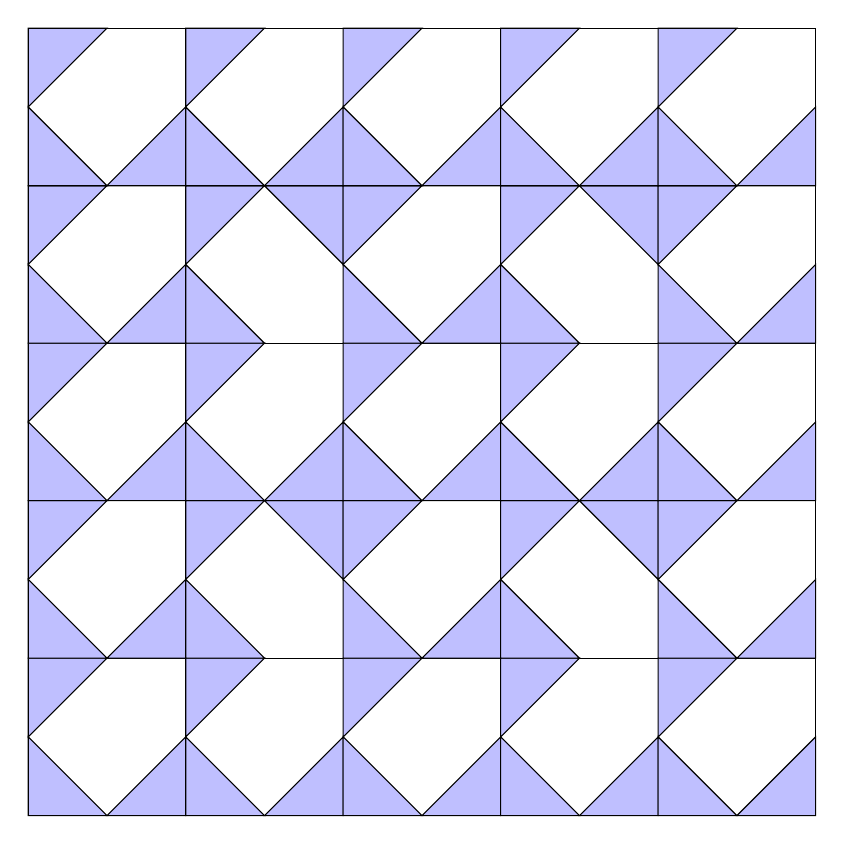
\begin{tikzpicture}
        				
					\bimcell

					\begin{scope}[xshift = 2cm, rotate = 0]
						\bimcell
					\end{scope}
					
					\begin{scope}[xshift = 4cm, rotate = 0]
						\bimcell
					\end{scope}

					\begin{scope}[xshift = 6cm, rotate = 0]
						\bimcell
					\end{scope}

					\begin{scope}[xshift = 8cm, rotate = 0]
						\bimcell
					\end{scope}
					
					\begin{scope}[yshift = 2cm, rotate = 0]
						\bimcell
					\end{scope}
					
					\begin{scope}[yshift = 2cm, xshift = 2cm, rotate = 270]
						\bimcell
					\end{scope}
					
					\begin{scope}[yshift = 2cm, xshift = 4cm, rotate = 0]
						\bimcell
					\end{scope}

					\begin{scope}[yshift = 2cm, xshift = 6cm, rotate = 270]
						\bimcell
					\end{scope}

					\begin{scope}[yshift = 2cm, xshift = 8cm, rotate = 0]
						\bimcell
					\end{scope}
					
					\begin{scope}[yshift = 4cm, rotate = 0]
						\bimcell
					\end{scope}
					
					\begin{scope}[yshift = 4cm, xshift = 2cm, rotate = 0]
						\bimcell
					\end{scope}
					
					\begin{scope}[yshift = 4cm, xshift = 4cm, rotate = 0]
						\bimcell
					\end{scope}

					\begin{scope}[yshift = 4cm, xshift = 6cm, rotate = 0]
						\bimcell
					\end{scope}

					\begin{scope}[yshift = 4cm, xshift = 8cm, rotate = 0]
						\bimcell
					\end{scope}
					
					\begin{scope}[yshift = 6cm, rotate = 0]
						\bimcell
					\end{scope}
					
					\begin{scope}[yshift = 6cm, xshift = 2cm, rotate = 270]
						\bimcell
					\end{scope}
					
					\begin{scope}[yshift = 6cm, xshift = 4cm, rotate = 0]
						\bimcell
					\end{scope}

					\begin{scope}[yshift = 6cm, xshift = 6cm, rotate = 270]
						\bimcell
					\end{scope}

					\begin{scope}[yshift = 6cm, xshift = 8cm, rotate = 0]
						\bimcell
					\end{scope}
					
					\begin{scope}[yshift = 8cm, rotate = 0]
						\bimcell
					\end{scope}
					
					\begin{scope}[yshift = 8cm, xshift = 2cm, rotate = 0]
						\bimcell
					\end{scope}
					
					\begin{scope}[yshift = 8cm, xshift = 4cm, rotate = 0]
						\bimcell
					\end{scope}

					\begin{scope}[yshift = 8cm, xshift = 6cm, rotate = 0]
						\bimcell				
					\end{scope}

					\begin{scope}[yshift = 8cm, xshift = 8cm, rotate = 0]
						\bimcell
					\end{scope}
										
				\end{tikzpicture}
				}
				\qquad\qquad
				\scalebox{0.35}{
				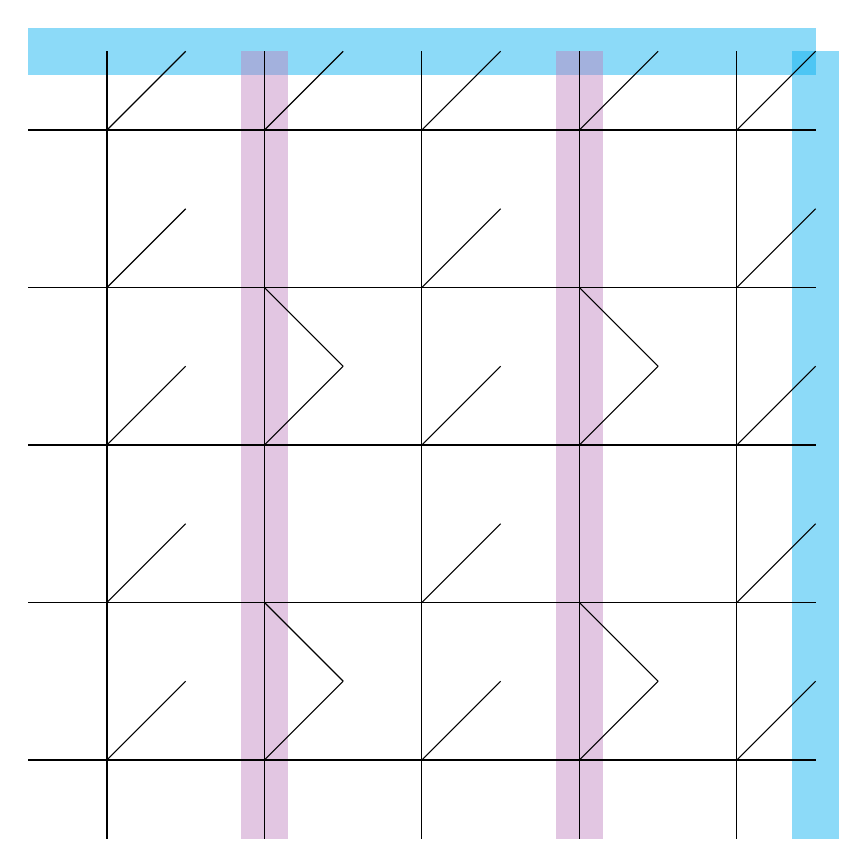
\begin{tikzpicture}
        			
					\begin{scope}[xshift = 9cm, rotate = 0]
						\bump
					\end{scope}
					
					\begin{scope}[yshift = 9cm, rotate = -90]
						\bump
					\end{scope}
					
					\begin{scope}[xshift = 2cm, rotate = 0]
						\domainwall
					\end{scope}
					
					\begin{scope}[xshift = 6cm, rotate = 0]
						\domainwall
					\end{scope}    			
        			
					\vertex

					\begin{scope}[xshift = 2cm, rotate = 0]
						\vertex
					\end{scope}
					
					\begin{scope}[xshift = 4cm, rotate = 0]
						\vertex
					\end{scope}

					\begin{scope}[xshift = 6cm, rotate = 0]
						\vertex
					\end{scope}

					\begin{scope}[xshift = 8cm, rotate = 0]
						\vertex
					\end{scope}
					
					\begin{scope}[yshift = 2cm, rotate = 0]
						\vertex
					\end{scope}
					
					\begin{scope}[yshift = 2cm, xshift = 2cm, rotate = 270]
						\vertex
					\end{scope}
					
					\begin{scope}[yshift = 2cm, xshift = 4cm, rotate = 0]
						\vertex
					\end{scope}

					\begin{scope}[yshift = 2cm, xshift = 6cm, rotate = 270]
						\vertex
					\end{scope}

					\begin{scope}[yshift = 2cm, xshift = 8cm, rotate = 0]
						\vertex
					\end{scope}
					
					\begin{scope}[yshift = 4cm, rotate = 0]
						\vertex
					\end{scope}
					
					\begin{scope}[yshift = 4cm, xshift = 2cm, rotate = 0]
						\vertex
					\end{scope}
					
					\begin{scope}[yshift = 4cm, xshift = 4cm, rotate = 0]
						\vertex
					\end{scope}

					\begin{scope}[yshift = 4cm, xshift = 6cm, rotate = 0]
						\vertex
					\end{scope}

					\begin{scope}[yshift = 4cm, xshift = 8cm, rotate = 0]
						\vertex
					\end{scope}
					
					\begin{scope}[yshift = 6cm, rotate = 0]
						\vertex
					\end{scope}
					
					\begin{scope}[yshift = 6cm, xshift = 2cm, rotate = 270]
						\vertex
					\end{scope}
					
					\begin{scope}[yshift = 6cm, xshift = 4cm, rotate = 0]
						\vertex
					\end{scope}

					\begin{scope}[yshift = 6cm, xshift = 6cm, rotate = 270]
						\vertex
					\end{scope}

					\begin{scope}[yshift = 6cm, xshift = 8cm, rotate = 0]
						\vertex
					\end{scope}
					
					\begin{scope}[yshift = 8cm, rotate = 0]
						\vertex
					\end{scope}
					
					\begin{scope}[yshift = 8cm, xshift = 2cm, rotate = 0]
						\vertex
					\end{scope}
					
					\begin{scope}[yshift = 8cm, xshift = 4cm, rotate = 0]
						\vertex
					\end{scope}

					\begin{scope}[yshift = 8cm, xshift = 6cm, rotate = 0]
						\vertex				
					\end{scope}

					\begin{scope}[yshift = 8cm, xshift = 8cm, rotate = 0]
						\vertex
					\end{scope}
										
				\end{tikzpicture}
				}
				}
				\caption{}
				\label{fig:p1}
			\end{figure}
			
			This tiling exhibits $p1$ symmetry. It admits bump modes along one direction but not the other. In addition, it may exhibit up to two surface shears, depending on whether the associated dimension is odd or even-numbered. Explicit listing for $n$ even yields $n/2+1$ mechanisms.
			
\subsection{Bump modes (p2)}
\label{sec:bumpy}

		
			\begin{figure}[!ht]
				\centering{
				\scalebox{0.35}{
				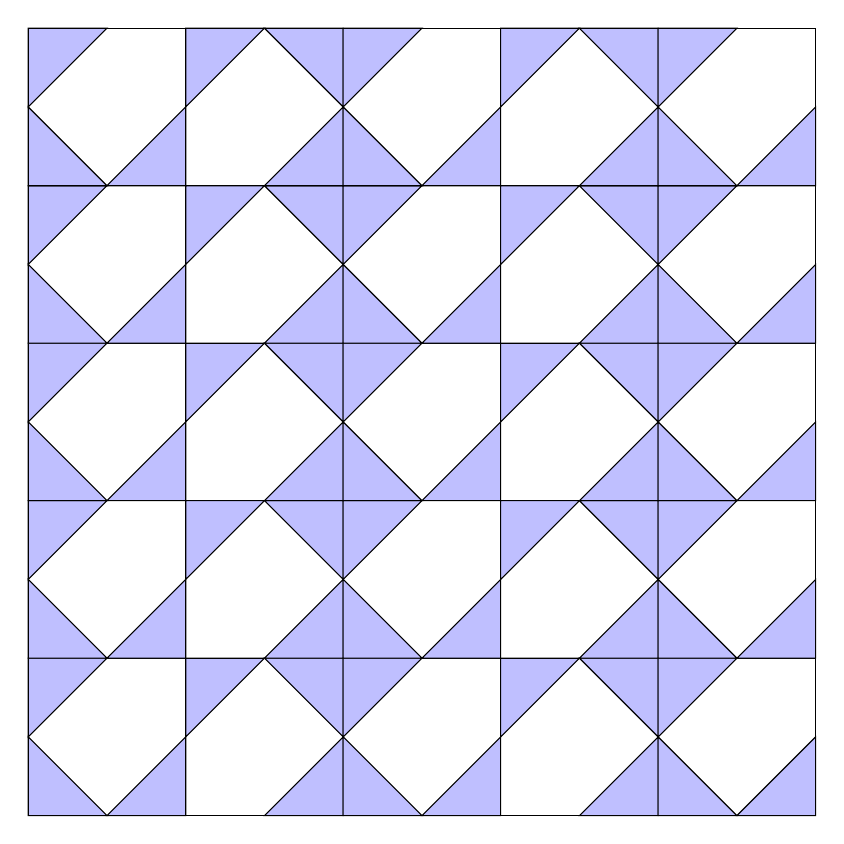
\begin{tikzpicture}
        				
					\bimcell

					\begin{scope}[xshift = 2cm, rotate = 180]
						\bimcell
					\end{scope}
					
					\begin{scope}[xshift = 4cm, rotate = 0]
						\bimcell
					\end{scope}

					\begin{scope}[xshift = 6cm, rotate = 180]
						\bimcell
					\end{scope}

					\begin{scope}[xshift = 8cm, rotate = 0]
						\bimcell
					\end{scope}
					
					\begin{scope}[yshift = 2cm, rotate = 0]
						\bimcell
					\end{scope}
					
					\begin{scope}[yshift = 2cm, xshift = 2cm, rotate = 180]
						\bimcell
					\end{scope}
					
					\begin{scope}[yshift = 2cm, xshift = 4cm, rotate = 0]
						\bimcell
					\end{scope}

					\begin{scope}[yshift = 2cm, xshift = 6cm, rotate = 180]
						\bimcell
					\end{scope}

					\begin{scope}[yshift = 2cm, xshift = 8cm, rotate = 0]
						\bimcell
					\end{scope}
					
					\begin{scope}[yshift = 4cm, rotate = 0]
						\bimcell
					\end{scope}
					
					\begin{scope}[yshift = 4cm, xshift = 2cm, rotate = 180]
						\bimcell
					\end{scope}
					
					\begin{scope}[yshift = 4cm, xshift = 4cm, rotate = 0]
						\bimcell
					\end{scope}

					\begin{scope}[yshift = 4cm, xshift = 6cm, rotate = 180]
						\bimcell
					\end{scope}

					\begin{scope}[yshift = 4cm, xshift = 8cm, rotate = 0]
						\bimcell
					\end{scope}
					
					\begin{scope}[yshift = 6cm, rotate = 0]
						\bimcell
					\end{scope}
					
					\begin{scope}[yshift = 6cm, xshift = 2cm, rotate = 180]
						\bimcell
					\end{scope}
					
					\begin{scope}[yshift = 6cm, xshift = 4cm, rotate = 0]
						\bimcell
					\end{scope}

					\begin{scope}[yshift = 6cm, xshift = 6cm, rotate = 180]
						\bimcell
					\end{scope}

					\begin{scope}[yshift = 6cm, xshift = 8cm, rotate = 0]
						\bimcell
					\end{scope}
					
					\begin{scope}[yshift = 8cm, rotate = 0]
						\bimcell
					\end{scope}
					
					\begin{scope}[yshift = 8cm, xshift = 2cm, rotate = 180]
						\bimcell
					\end{scope}
					
					\begin{scope}[yshift = 8cm, xshift = 4cm, rotate = 0]
						\bimcell
					\end{scope}

					\begin{scope}[yshift = 8cm, xshift = 6cm, rotate = 180]
						\bimcell				
					\end{scope}

					\begin{scope}[yshift = 8cm, xshift = 8cm, rotate = 0]
						\bimcell
					\end{scope}
										
				\end{tikzpicture}
				}
				\qquad
				\qquad
				\scalebox{0.35}{
				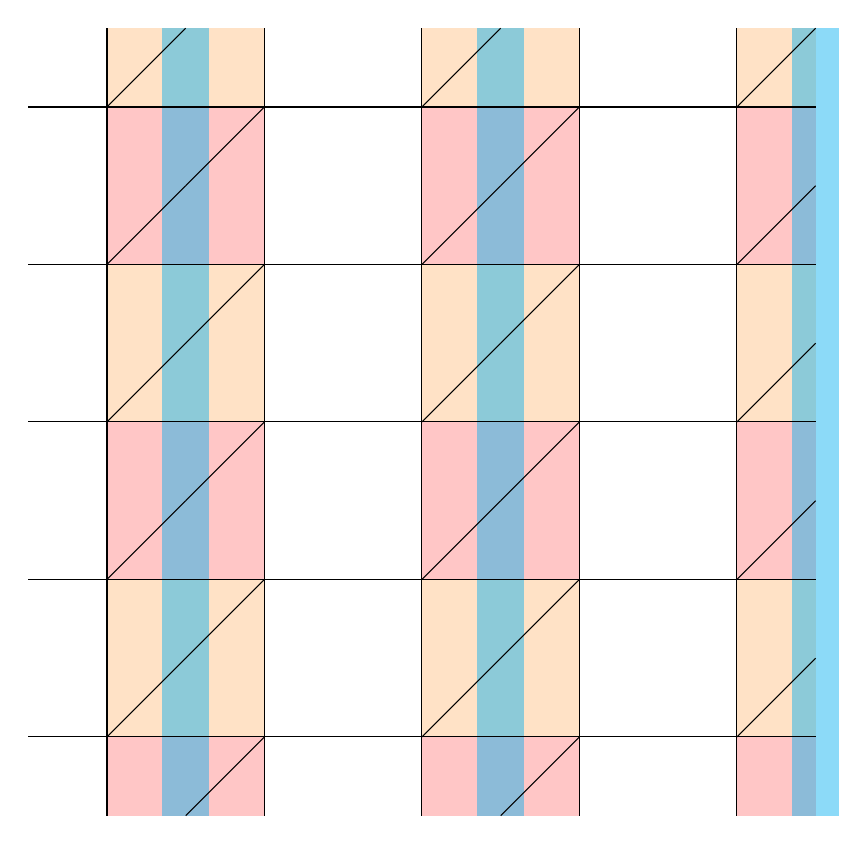
\begin{tikzpicture}
				
					\lindeca
				
					\begin{scope}[xshift = 0cm, yshift=8cm, rotate = -90]
						\lindecb
					\end{scope}
				
					\begin{scope}[xshift = 1cm, rotate = 0]
						\bump
					\end{scope}
					
					\begin{scope}[xshift = 5cm, rotate = 0]
						\bump
					\end{scope}
					
					\begin{scope}[xshift = 9cm, rotate = 0]
						\bump
					\end{scope}
        				
					\vertex

					\begin{scope}[xshift = 2cm, rotate = 180]
						\vertex
					\end{scope}
					
					\begin{scope}[xshift = 4cm, rotate = 0]
						\vertex
					\end{scope}

					\begin{scope}[xshift = 6cm, rotate = 180]
						\vertex
					\end{scope}

					\begin{scope}[xshift = 8cm, rotate = 0]
						\vertex
					\end{scope}
					
					\begin{scope}[yshift = 2cm, rotate = 0]
						\vertex
					\end{scope}
					
					\begin{scope}[yshift = 2cm, xshift = 2cm, rotate = 180]
						\vertex
					\end{scope}
					
					\begin{scope}[yshift = 2cm, xshift = 4cm, rotate = 0]
						\vertex
					\end{scope}

					\begin{scope}[yshift = 2cm, xshift = 6cm, rotate = 180]
						\vertex
					\end{scope}

					\begin{scope}[yshift = 2cm, xshift = 8cm, rotate = 0]
						\vertex
					\end{scope}
					
					\begin{scope}[yshift = 4cm, rotate = 0]
						\vertex
					\end{scope}
					
					\begin{scope}[yshift = 4cm, xshift = 2cm, rotate = 180]
						\vertex
					\end{scope}
					
					\begin{scope}[yshift = 4cm, xshift = 4cm, rotate = 0]
						\vertex
					\end{scope}

					\begin{scope}[yshift = 4cm, xshift = 6cm, rotate = 180]
						\vertex
					\end{scope}

					\begin{scope}[yshift = 4cm, xshift = 8cm, rotate = 0]
						\vertex
					\end{scope}
					
					\begin{scope}[yshift = 6cm, rotate = 0]
						\vertex
					\end{scope}
					
					\begin{scope}[yshift = 6cm, xshift = 2cm, rotate = 180]
						\vertex
					\end{scope}
					
					\begin{scope}[yshift = 6cm, xshift = 4cm, rotate = 0]
						\vertex
					\end{scope}

					\begin{scope}[yshift = 6cm, xshift = 6cm, rotate = 180]
						\vertex
					\end{scope}

					\begin{scope}[yshift = 6cm, xshift = 8cm, rotate = 0]
						\vertex
					\end{scope}
					
					\begin{scope}[yshift = 8cm, rotate = 0]
						\vertex
					\end{scope}
					
					\begin{scope}[yshift = 8cm, xshift = 2cm, rotate = 180]
						\vertex
					\end{scope}
					
					\begin{scope}[yshift = 8cm, xshift = 4cm, rotate = 0]
						\vertex
					\end{scope}

					\begin{scope}[yshift = 8cm, xshift = 6cm, rotate = 180]
						\vertex				
					\end{scope}

					\begin{scope}[yshift = 8cm, xshift = 8cm, rotate = 0]
						\vertex
					\end{scope}
										
				\end{tikzpicture}
				}
				}
				\caption{A tiling that admits a number of modes scaling with the perimeter.}
				\label{fig:bumpy}
			\end{figure}
			
			This tiling exhibits $p2$ symmetry. It admits bump modes along one direction but not the other. In addition, it possesses two linear decay sublattices, thus allowing for the four associated linear decay modes. Explicit listing for $n$ even yields $n/2 + 4$ mechanisms. As shown in Fig.\ref{fig:san:p2}, this overcounts the modes by two. We can guess that the four linear decay mechanisms are actually two, because they have the same orientation. 
			
\subsection{(pm)}
\label{sec:pm}

		
			\begin{figure}[!ht]
				\centering{
				\scalebox{0.35}{
				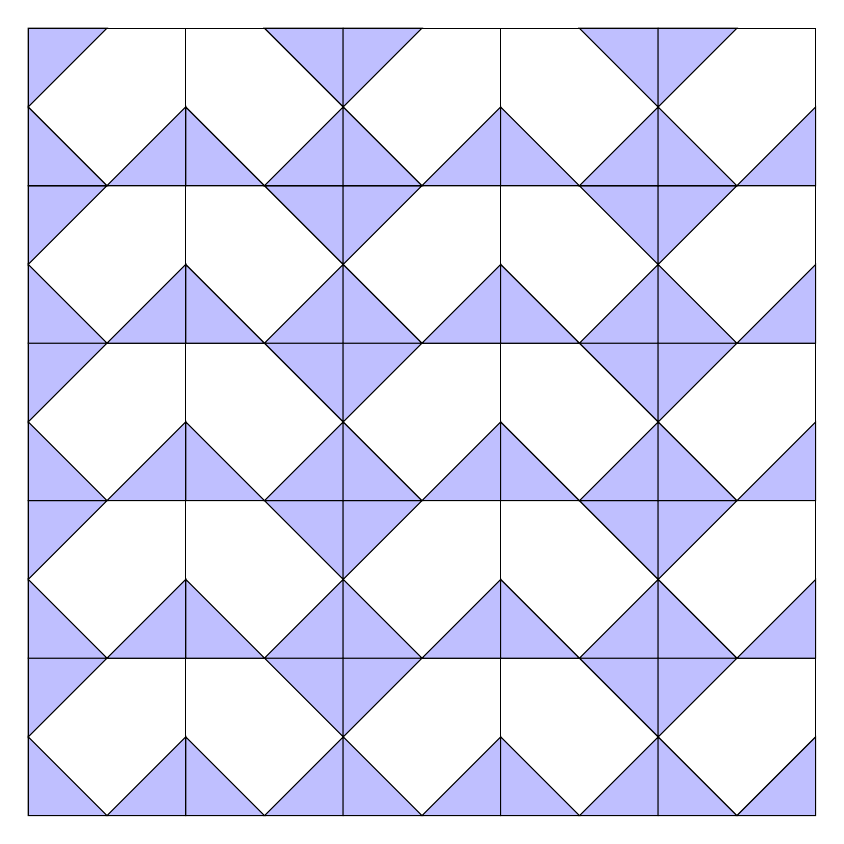
\begin{tikzpicture}
        				
					\bimcell

					\begin{scope}[xshift = 2cm, rotate = 90]
						\bimcell
					\end{scope}
					
					\begin{scope}[xshift = 4cm, rotate = 0]
						\bimcell
					\end{scope}

					\begin{scope}[xshift = 6cm, rotate = 90]
						\bimcell
					\end{scope}

					\begin{scope}[xshift = 8cm, rotate = 0]
						\bimcell
					\end{scope}
					
					\begin{scope}[yshift = 2cm, rotate = 0]
						\bimcell
					\end{scope}
					
					\begin{scope}[yshift = 2cm, xshift = 2cm, rotate = 90]
						\bimcell
					\end{scope}
					
					\begin{scope}[yshift = 2cm, xshift = 4cm, rotate = 0]
						\bimcell
					\end{scope}

					\begin{scope}[yshift = 2cm, xshift = 6cm, rotate = 90]
						\bimcell
					\end{scope}

					\begin{scope}[yshift = 2cm, xshift = 8cm, rotate = 0]
						\bimcell
					\end{scope}
					
					\begin{scope}[yshift = 4cm, rotate = 0]
						\bimcell
					\end{scope}
					
					\begin{scope}[yshift = 4cm, xshift = 2cm, rotate = 90]
						\bimcell
					\end{scope}
					
					\begin{scope}[yshift = 4cm, xshift = 4cm, rotate = 0]
						\bimcell
					\end{scope}

					\begin{scope}[yshift = 4cm, xshift = 6cm, rotate = 90]
						\bimcell
					\end{scope}

					\begin{scope}[yshift = 4cm, xshift = 8cm, rotate = 0]
						\bimcell
					\end{scope}
					
					\begin{scope}[yshift = 6cm, rotate = 0]
						\bimcell
					\end{scope}
					
					\begin{scope}[yshift = 6cm, xshift = 2cm, rotate = 90]
						\bimcell
					\end{scope}
					
					\begin{scope}[yshift = 6cm, xshift = 4cm, rotate = 0]
						\bimcell
					\end{scope}

					\begin{scope}[yshift = 6cm, xshift = 6cm, rotate = 90]
						\bimcell
					\end{scope}

					\begin{scope}[yshift = 6cm, xshift = 8cm, rotate = 0]
						\bimcell
					\end{scope}
					
					\begin{scope}[yshift = 8cm, rotate = 0]
						\bimcell
					\end{scope}
					
					\begin{scope}[yshift = 8cm, xshift = 2cm, rotate = 90]
						\bimcell
					\end{scope}
					
					\begin{scope}[yshift = 8cm, xshift = 4cm, rotate = 0]
						\bimcell
					\end{scope}

					\begin{scope}[yshift = 8cm, xshift = 6cm, rotate = 90]
						\bimcell				
					\end{scope}

					\begin{scope}[yshift = 8cm, xshift = 8cm, rotate = 0]
						\bimcell
					\end{scope}
										
				\end{tikzpicture}
				}
				\qquad
				\qquad
				\scalebox{0.35}{
				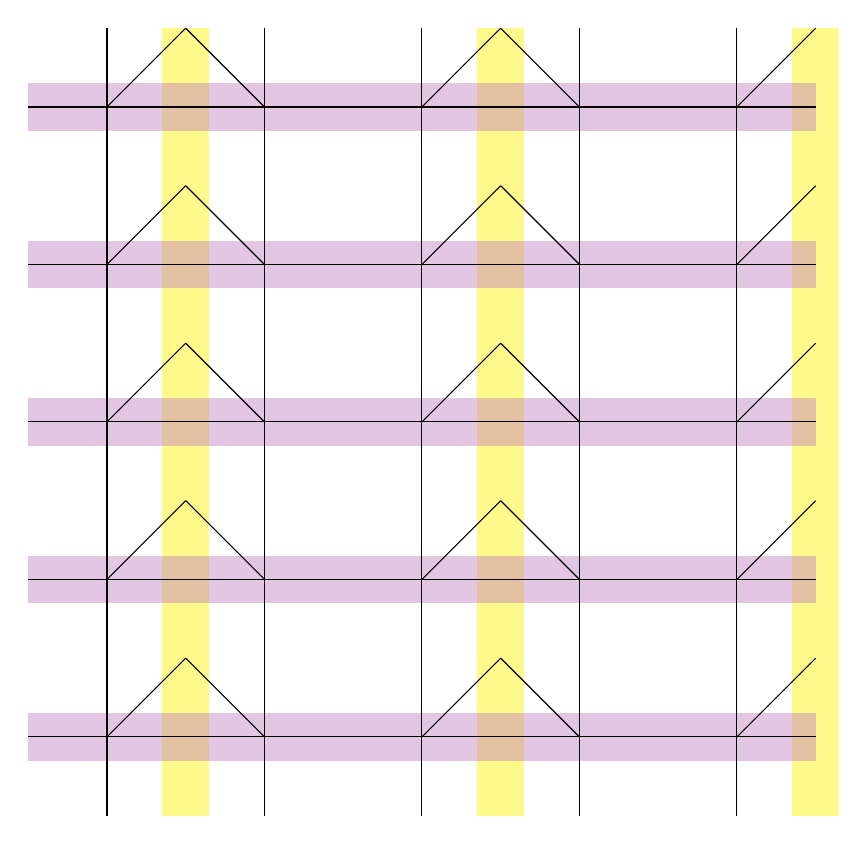
\begin{tikzpicture}
				
					\begin{scope}[xshift = 1cm, rotate = 0]
						\antibump
					\end{scope}
					
					\begin{scope}[xshift = 5cm, rotate = 0]
						\antibump
					\end{scope}
					
					\begin{scope}[xshift = 9cm, rotate = 0]
						\antibump
					\end{scope}
					
					\begin{scope}[yshift = 0cm, rotate = -90]
						\domainwall
					\end{scope}
					
					\begin{scope}[yshift = 2cm, rotate = -90]
						\domainwall
					\end{scope}
					
					\begin{scope}[yshift = 4cm, rotate = -90]
						\domainwall
					\end{scope}
					
					\begin{scope}[yshift = 6cm, rotate = -90]
						\domainwall
					\end{scope}
					
					\begin{scope}[yshift = 8cm, rotate = -90]
						\domainwall
					\end{scope}
        				
					\vertex

					\begin{scope}[xshift = 2cm, rotate = 90]
						\vertex
					\end{scope}
					
					\begin{scope}[xshift = 4cm, rotate = 0]
						\vertex
					\end{scope}

					\begin{scope}[xshift = 6cm, rotate = 90]
						\vertex
					\end{scope}

					\begin{scope}[xshift = 8cm, rotate = 0]
						\vertex
					\end{scope}
					
					\begin{scope}[yshift = 2cm, rotate = 0]
						\vertex
					\end{scope}
					
					\begin{scope}[yshift = 2cm, xshift = 2cm, rotate = 90]
						\vertex
					\end{scope}
					
					\begin{scope}[yshift = 2cm, xshift = 4cm, rotate = 0]
						\vertex
					\end{scope}

					\begin{scope}[yshift = 2cm, xshift = 6cm, rotate = 90]
						\vertex
					\end{scope}

					\begin{scope}[yshift = 2cm, xshift = 8cm, rotate = 0]
						\vertex
					\end{scope}
					
					\begin{scope}[yshift = 4cm, rotate = 0]
						\vertex
					\end{scope}
					
					\begin{scope}[yshift = 4cm, xshift = 2cm, rotate = 90]
						\vertex
					\end{scope}
					
					\begin{scope}[yshift = 4cm, xshift = 4cm, rotate = 0]
						\vertex
					\end{scope}

					\begin{scope}[yshift = 4cm, xshift = 6cm, rotate = 90]
						\vertex
					\end{scope}

					\begin{scope}[yshift = 4cm, xshift = 8cm, rotate = 0]
						\vertex
					\end{scope}
					
					\begin{scope}[yshift = 6cm, rotate = 0]
						\vertex
					\end{scope}
					
					\begin{scope}[yshift = 6cm, xshift = 2cm, rotate = 90]
						\vertex
					\end{scope}
					
					\begin{scope}[yshift = 6cm, xshift = 4cm, rotate = 0]
						\vertex
					\end{scope}

					\begin{scope}[yshift = 6cm, xshift = 6cm, rotate = 90]
						\vertex
					\end{scope}

					\begin{scope}[yshift = 6cm, xshift = 8cm, rotate = 0]
						\vertex
					\end{scope}
					
					\begin{scope}[yshift = 8cm, rotate = 0]
						\vertex
					\end{scope}
					
					\begin{scope}[yshift = 8cm, xshift = 2cm, rotate = 90]
						\vertex
					\end{scope}
					
					\begin{scope}[yshift = 8cm, xshift = 4cm, rotate = 0]
						\vertex
					\end{scope}

					\begin{scope}[yshift = 8cm, xshift = 6cm, rotate = 90]
						\vertex				
					\end{scope}

					\begin{scope}[yshift = 8cm, xshift = 8cm, rotate = 0]
						\vertex
					\end{scope}
										
				\end{tikzpicture}
				}
				}
				\caption{pm}
				\label{fig:pm}
			\end{figure}
			
			This tiling exhibits $pm$ symmetry. It admits bump modes along one direction but not the other. In addition, it may exhibit up to one surface shear, depending on whether $n$ is odd or even. Explicit listing for $n$ even yields $n/2+m+1$ mechanisms. As shown in Fig.\ref{fig:san:pm}, this overcounts the modes by one. Can we explain that?
			
\subsection{(cm:1)}
\label{sec:cm:1}

		
			\begin{figure}[!ht]
				\centering{
				\scalebox{0.35}{
				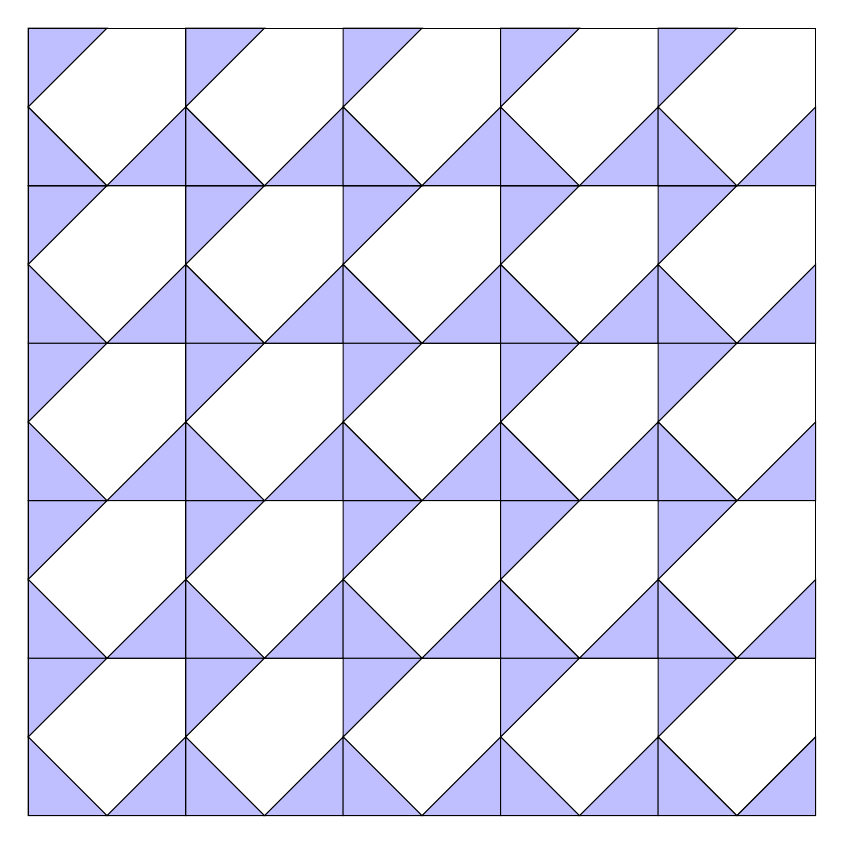
\begin{tikzpicture}
        				
					\bimcell

					\begin{scope}[xshift = 2cm, rotate = 0]
						\bimcell
					\end{scope}
					
					\begin{scope}[xshift = 4cm, rotate = 0]
						\bimcell
					\end{scope}

					\begin{scope}[xshift = 6cm, rotate = 0]
						\bimcell
					\end{scope}

					\begin{scope}[xshift = 8cm, rotate = 0]
						\bimcell
					\end{scope}
					
					\begin{scope}[yshift = 2cm, rotate = 0]
						\bimcell
					\end{scope}
					
					\begin{scope}[yshift = 2cm, xshift = 2cm, rotate = 0]
						\bimcell
					\end{scope}
					
					\begin{scope}[yshift = 2cm, xshift = 4cm, rotate = 0]
						\bimcell
					\end{scope}

					\begin{scope}[yshift = 2cm, xshift = 6cm, rotate = 0]
						\bimcell
					\end{scope}

					\begin{scope}[yshift = 2cm, xshift = 8cm, rotate = 0]
						\bimcell
					\end{scope}
					
					\begin{scope}[yshift = 4cm, rotate = 0]
						\bimcell
					\end{scope}
					
					\begin{scope}[yshift = 4cm, xshift = 2cm, rotate = 0]
						\bimcell
					\end{scope}
					
					\begin{scope}[yshift = 4cm, xshift = 4cm, rotate = 0]
						\bimcell
					\end{scope}

					\begin{scope}[yshift = 4cm, xshift = 6cm, rotate = 0]
						\bimcell
					\end{scope}

					\begin{scope}[yshift = 4cm, xshift = 8cm, rotate = 0]
						\bimcell
					\end{scope}
					
					\begin{scope}[yshift = 6cm, rotate = 0]
						\bimcell
					\end{scope}
					
					\begin{scope}[yshift = 6cm, xshift = 2cm, rotate = 0]
						\bimcell
					\end{scope}
					
					\begin{scope}[yshift = 6cm, xshift = 4cm, rotate = 0]
						\bimcell
					\end{scope}

					\begin{scope}[yshift = 6cm, xshift = 6cm, rotate = 0]
						\bimcell
					\end{scope}

					\begin{scope}[yshift = 6cm, xshift = 8cm, rotate = 0]
						\bimcell
					\end{scope}
					
					\begin{scope}[yshift = 8cm, rotate = 0]
						\bimcell
					\end{scope}
					
					\begin{scope}[yshift = 8cm, xshift = 2cm, rotate = 0]
						\bimcell
					\end{scope}
					
					\begin{scope}[yshift = 8cm, xshift = 4cm, rotate = 0]
						\bimcell
					\end{scope}

					\begin{scope}[yshift = 8cm, xshift = 6cm, rotate = 0]
						\bimcell				
					\end{scope}

					\begin{scope}[yshift = 8cm, xshift = 8cm, rotate = 0]
						\bimcell
					\end{scope}
										
				\end{tikzpicture}
				}
				\qquad
				\qquad
				\scalebox{0.35}{
				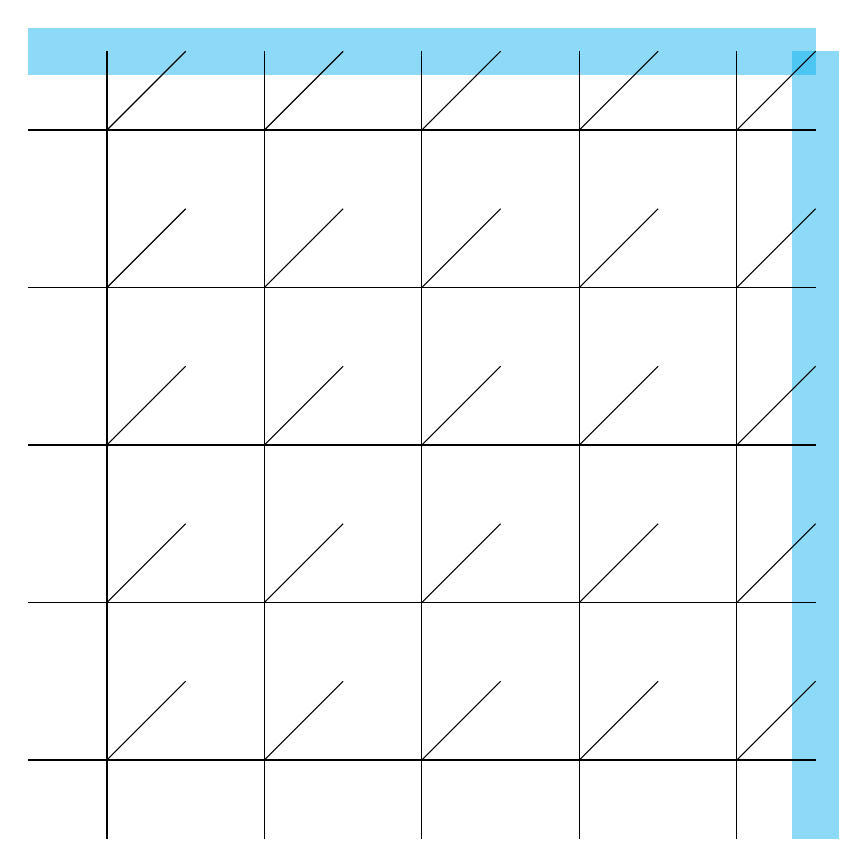
\begin{tikzpicture}
				
					\begin{scope}[xshift = 9cm, rotate = 0]
						\bump
					\end{scope}
					
					\begin{scope}[yshift = 9cm, rotate = -90]
						\bump
					\end{scope}
        				
					\vertex

					\begin{scope}[xshift = 2cm, rotate = 0]
						\vertex
					\end{scope}
					
					\begin{scope}[xshift = 4cm, rotate = 0]
						\vertex
					\end{scope}

					\begin{scope}[xshift = 6cm, rotate = 0]
						\vertex
					\end{scope}

					\begin{scope}[xshift = 8cm, rotate = 0]
						\vertex
					\end{scope}
					
					\begin{scope}[yshift = 2cm, rotate = 0]
						\vertex
					\end{scope}
					
					\begin{scope}[yshift = 2cm, xshift = 2cm, rotate = 0]
						\vertex
					\end{scope}
					
					\begin{scope}[yshift = 2cm, xshift = 4cm, rotate = 0]
						\vertex
					\end{scope}

					\begin{scope}[yshift = 2cm, xshift = 6cm, rotate = 0]
						\vertex
					\end{scope}

					\begin{scope}[yshift = 2cm, xshift = 8cm, rotate = 0]
						\vertex
					\end{scope}
					
					\begin{scope}[yshift = 4cm, rotate = 0]
						\vertex
					\end{scope}
					
					\begin{scope}[yshift = 4cm, xshift = 2cm, rotate = 0]
						\vertex
					\end{scope}
					
					\begin{scope}[yshift = 4cm, xshift = 4cm, rotate = 0]
						\vertex
					\end{scope}

					\begin{scope}[yshift = 4cm, xshift = 6cm, rotate = 0]
						\vertex
					\end{scope}

					\begin{scope}[yshift = 4cm, xshift = 8cm, rotate = 0]
						\vertex
					\end{scope}
					
					\begin{scope}[yshift = 6cm, rotate = 0]
						\vertex
					\end{scope}
					
					\begin{scope}[yshift = 6cm, xshift = 2cm, rotate = 0]
						\vertex
					\end{scope}
					
					\begin{scope}[yshift = 6cm, xshift = 4cm, rotate = 0]
						\vertex
					\end{scope}

					\begin{scope}[yshift = 6cm, xshift = 6cm, rotate = 0]
						\vertex
					\end{scope}

					\begin{scope}[yshift = 6cm, xshift = 8cm, rotate = 0]
						\vertex
					\end{scope}
					
					\begin{scope}[yshift = 8cm, rotate = 0]
						\vertex
					\end{scope}
					
					\begin{scope}[yshift = 8cm, xshift = 2cm, rotate = 0]
						\vertex
					\end{scope}
					
					\begin{scope}[yshift = 8cm, xshift = 4cm, rotate = 0]
						\vertex
					\end{scope}

					\begin{scope}[yshift = 8cm, xshift = 6cm, rotate = 0]
						\vertex				
					\end{scope}

					\begin{scope}[yshift = 8cm, xshift = 8cm, rotate = 0]
						\vertex
					\end{scope}
										
				\end{tikzpicture}
				}
				}
				\caption{}
				\label{fig:cm:1}
			\end{figure}
			
			This tiling exhibits $cm$ symmetry. It only admits counter-rotations and two surface shears, totalling three mechanisms. A variant of this tiling with only one mechanism will be described in subsection \ref{sec:crmode}, reflecting a general design principle for surface shear modes.

\subsection{(cm:2)}
\label{sec:cm:2}

		
			\begin{figure}[!ht]
				\centering{
				\scalebox{0.35}{
				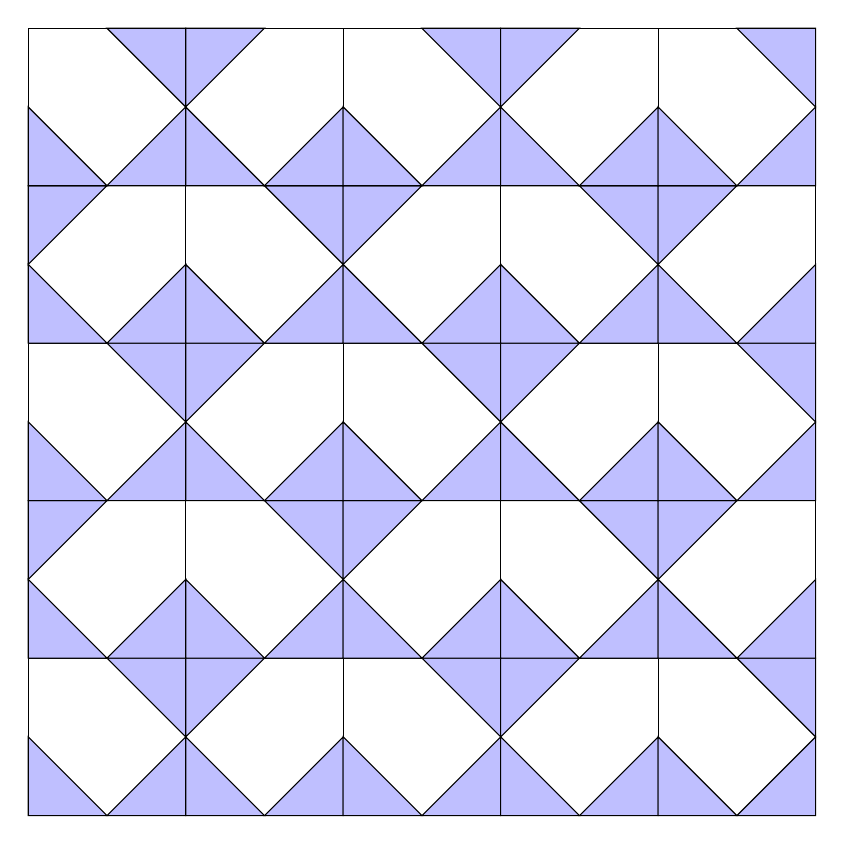
\begin{tikzpicture}
        				
					\begin{scope}[xshift = 0cm, rotate = 90]
						\bimcell
					\end{scope}
					
					\begin{scope}[xshift = 2cm, rotate = 0]
						\bimcell
					\end{scope}
					
					\begin{scope}[xshift = 4cm, rotate = 90]
						\bimcell
					\end{scope}

					\begin{scope}[xshift = 6cm, rotate = 0]
						\bimcell
					\end{scope}

					\begin{scope}[xshift = 8cm, rotate = 90]
						\bimcell
					\end{scope}
					
					\begin{scope}[yshift = 2cm, rotate = 0]
						\bimcell
					\end{scope}
					
					\begin{scope}[yshift = 2cm, xshift = 2cm, rotate = 90]
						\bimcell
					\end{scope}
					
					\begin{scope}[yshift = 2cm, xshift = 4cm, rotate = 0]
						\bimcell
					\end{scope}

					\begin{scope}[yshift = 2cm, xshift = 6cm, rotate = 90]
						\bimcell
					\end{scope}

					\begin{scope}[yshift = 2cm, xshift = 8cm, rotate = 0]
						\bimcell
					\end{scope}
					
					\begin{scope}[yshift = 4cm, rotate = 90]
						\bimcell
					\end{scope}
					
					\begin{scope}[yshift = 4cm, xshift = 2cm, rotate = 0]
						\bimcell
					\end{scope}
					
					\begin{scope}[yshift = 4cm, xshift = 4cm, rotate = 90]
						\bimcell
					\end{scope}

					\begin{scope}[yshift = 4cm, xshift = 6cm, rotate = 0]
						\bimcell
					\end{scope}

					\begin{scope}[yshift = 4cm, xshift = 8cm, rotate = 90]
						\bimcell
					\end{scope}
					
					\begin{scope}[yshift = 6cm, rotate = 0]
						\bimcell
					\end{scope}
					
					\begin{scope}[yshift = 6cm, xshift = 2cm, rotate = 90]
						\bimcell
					\end{scope}
					
					\begin{scope}[yshift = 6cm, xshift = 4cm, rotate = 0]
						\bimcell
					\end{scope}

					\begin{scope}[yshift = 6cm, xshift = 6cm, rotate = 90]
						\bimcell
					\end{scope}

					\begin{scope}[yshift = 6cm, xshift = 8cm, rotate = 0]
						\bimcell
					\end{scope}
					
					\begin{scope}[yshift = 8cm, rotate = 90]
						\bimcell
					\end{scope}
					
					\begin{scope}[yshift = 8cm, xshift = 2cm, rotate = 0]
						\bimcell
					\end{scope}
					
					\begin{scope}[yshift = 8cm, xshift = 4cm, rotate = 90]
						\bimcell
					\end{scope}

					\begin{scope}[yshift = 8cm, xshift = 6cm, rotate = 0]
						\bimcell				
					\end{scope}

					\begin{scope}[yshift = 8cm, xshift = 8cm, rotate = 90]
						\bimcell
					\end{scope}
										
				\end{tikzpicture}
				}
				\qquad
				\qquad
				\scalebox{0.35}{
				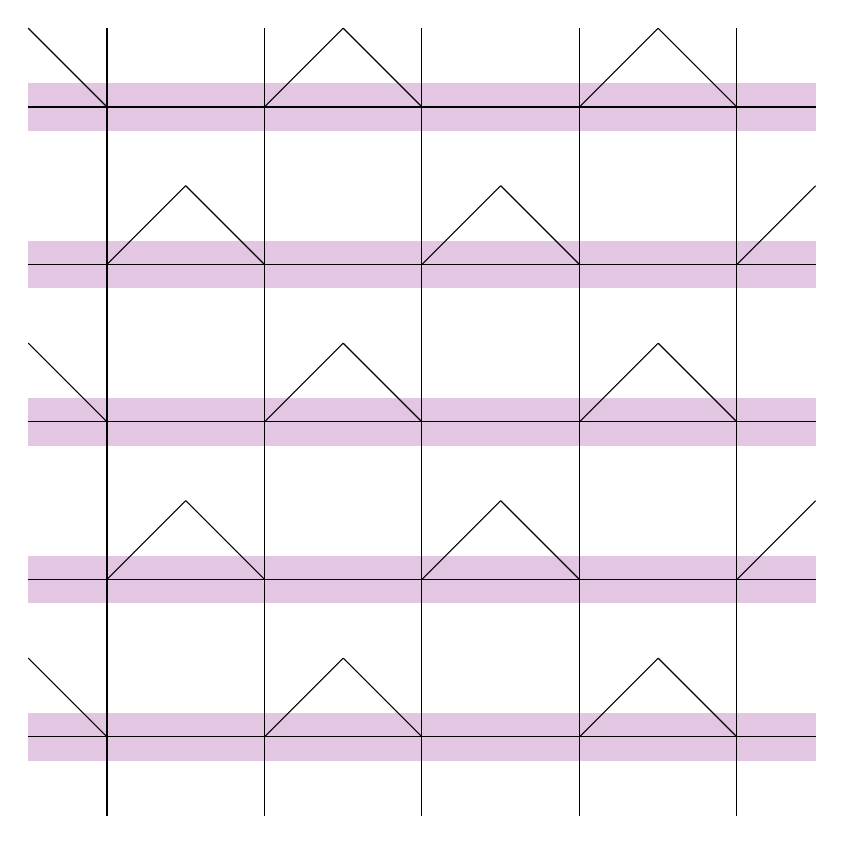
\begin{tikzpicture}
					
					\begin{scope}[yshift = 0cm, rotate = -90]
						\domainwall
					\end{scope}
					
					\begin{scope}[yshift = 2cm, rotate = -90]
						\domainwall
					\end{scope}
					
					\begin{scope}[yshift = 4cm, rotate = -90]
						\domainwall
					\end{scope}
					
					\begin{scope}[yshift = 6cm, rotate = -90]
						\domainwall
					\end{scope}
					
					\begin{scope}[yshift = 8cm, rotate = -90]
						\domainwall
					\end{scope}
        				
					\begin{scope}[xshift = 0cm, rotate = 90]
						\vertex
					\end{scope}
					
					\begin{scope}[xshift = 2cm, rotate = 0]
						\vertex
					\end{scope}
					
					\begin{scope}[xshift = 4cm, rotate = 90]
						\vertex
					\end{scope}

					\begin{scope}[xshift = 6cm, rotate = 0]
						\vertex
					\end{scope}

					\begin{scope}[xshift = 8cm, rotate = 90]
						\vertex
					\end{scope}
					
					\begin{scope}[yshift = 2cm, rotate = 0]
						\vertex
					\end{scope}
					
					\begin{scope}[yshift = 2cm, xshift = 2cm, rotate = 90]
						\vertex
					\end{scope}
					
					\begin{scope}[yshift = 2cm, xshift = 4cm, rotate = 0]
						\vertex
					\end{scope}

					\begin{scope}[yshift = 2cm, xshift = 6cm, rotate = 90]
						\vertex
					\end{scope}

					\begin{scope}[yshift = 2cm, xshift = 8cm, rotate = 0]
						\vertex
					\end{scope}
					
					\begin{scope}[yshift = 4cm, rotate = 90]
						\vertex
					\end{scope}
					
					\begin{scope}[yshift = 4cm, xshift = 2cm, rotate = 0]
						\vertex
					\end{scope}
					
					\begin{scope}[yshift = 4cm, xshift = 4cm, rotate = 90]
						\vertex
					\end{scope}

					\begin{scope}[yshift = 4cm, xshift = 6cm, rotate = 0]
						\vertex
					\end{scope}

					\begin{scope}[yshift = 4cm, xshift = 8cm, rotate = 90]
						\vertex
					\end{scope}
					
					\begin{scope}[yshift = 6cm, rotate = 0]
						\vertex
					\end{scope}
					
					\begin{scope}[yshift = 6cm, xshift = 2cm, rotate = 90]
						\vertex
					\end{scope}
					
					\begin{scope}[yshift = 6cm, xshift = 4cm, rotate = 0]
						\vertex
					\end{scope}

					\begin{scope}[yshift = 6cm, xshift = 6cm, rotate = 90]
						\vertex
					\end{scope}

					\begin{scope}[yshift = 6cm, xshift = 8cm, rotate = 0]
						\vertex
					\end{scope}
					
					\begin{scope}[yshift = 8cm, rotate = 90]
						\vertex
					\end{scope}
					
					\begin{scope}[yshift = 8cm, xshift = 2cm, rotate = 0]
						\vertex
					\end{scope}
					
					\begin{scope}[yshift = 8cm, xshift = 4cm, rotate = 90]
						\vertex
					\end{scope}

					\begin{scope}[yshift = 8cm, xshift = 6cm, rotate = 0]
						\vertex				
					\end{scope}

					\begin{scope}[yshift = 8cm, xshift = 8cm, rotate = 90]
						\vertex
					\end{scope}
										
				\end{tikzpicture}
				}
				}
				\caption{Another cm}
				\label{fig:cm:2}
			\end{figure}
			
			This tiling also exhibits $cm$ symmetry, albeit with a greater period. It admits domain-wall modes along one direction but not the other. Explicit listing for $n$ and $m$ even yields $m+1$ mechanisms.
			
			
\subsection{(cm:3)}
\label{sec:cm:3}

		
			\begin{figure}[!ht]
				\centering{
				\scalebox{0.35}{
				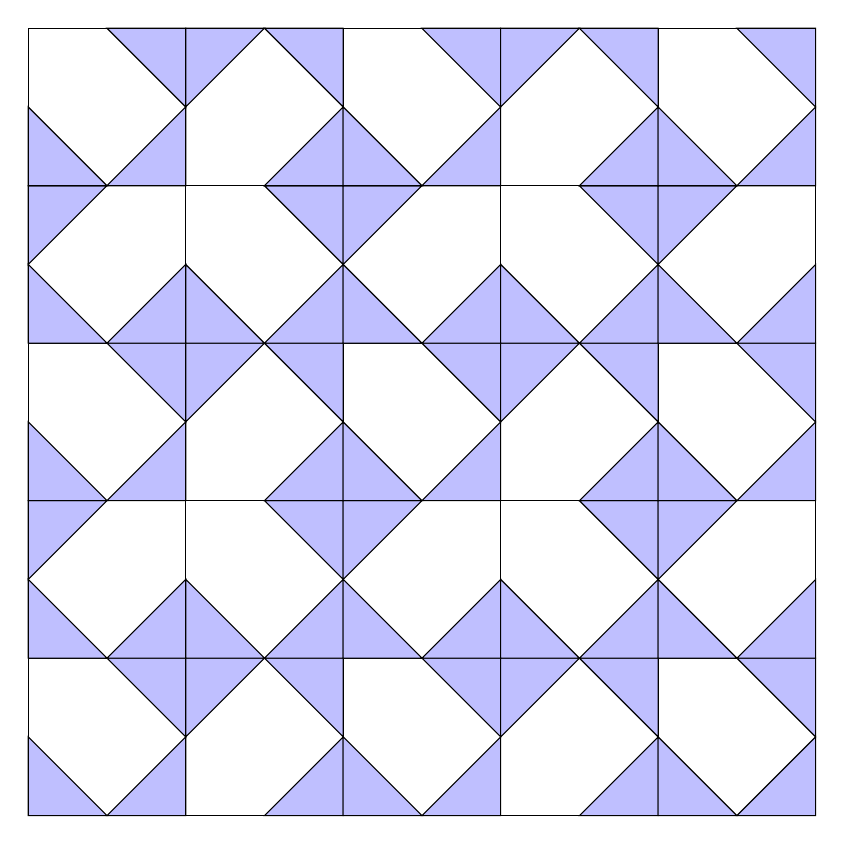
\begin{tikzpicture}
        				
					\begin{scope}[xshift = 0cm, rotate = 90]
						\bimcell
					\end{scope}
					
					\begin{scope}[xshift = 2cm, rotate = 180]
						\bimcell
					\end{scope}
					
					\begin{scope}[xshift = 4cm, rotate = 90]
						\bimcell
					\end{scope}

					\begin{scope}[xshift = 6cm, rotate = 180]
						\bimcell
					\end{scope}

					\begin{scope}[xshift = 8cm, rotate = 90]
						\bimcell
					\end{scope}
					
					\begin{scope}[yshift = 2cm, rotate = 0]
						\bimcell
					\end{scope}
					
					\begin{scope}[yshift = 2cm, xshift = 2cm, rotate = 90]
						\bimcell
					\end{scope}
					
					\begin{scope}[yshift = 2cm, xshift = 4cm, rotate = 0]
						\bimcell
					\end{scope}

					\begin{scope}[yshift = 2cm, xshift = 6cm, rotate = 90]
						\bimcell
					\end{scope}

					\begin{scope}[yshift = 2cm, xshift = 8cm, rotate = 0]
						\bimcell
					\end{scope}
					
					\begin{scope}[yshift = 4cm, rotate = 90]
						\bimcell
					\end{scope}
					
					\begin{scope}[yshift = 4cm, xshift = 2cm, rotate = 180]
						\bimcell
					\end{scope}
					
					\begin{scope}[yshift = 4cm, xshift = 4cm, rotate = 90]
						\bimcell
					\end{scope}

					\begin{scope}[yshift = 4cm, xshift = 6cm, rotate = 180]
						\bimcell
					\end{scope}

					\begin{scope}[yshift = 4cm, xshift = 8cm, rotate = 90]
						\bimcell
					\end{scope}
					
					\begin{scope}[yshift = 6cm, rotate = 0]
						\bimcell
					\end{scope}
					
					\begin{scope}[yshift = 6cm, xshift = 2cm, rotate = 90]
						\bimcell
					\end{scope}
					
					\begin{scope}[yshift = 6cm, xshift = 4cm, rotate = 0]
						\bimcell
					\end{scope}

					\begin{scope}[yshift = 6cm, xshift = 6cm, rotate = 90]
						\bimcell
					\end{scope}

					\begin{scope}[yshift = 6cm, xshift = 8cm, rotate = 0]
						\bimcell
					\end{scope}
					
					\begin{scope}[yshift = 8cm, rotate = 90]
						\bimcell
					\end{scope}
					
					\begin{scope}[yshift = 8cm, xshift = 2cm, rotate = 180]
						\bimcell
					\end{scope}
					
					\begin{scope}[yshift = 8cm, xshift = 4cm, rotate = 90]
						\bimcell
					\end{scope}

					\begin{scope}[yshift = 8cm, xshift = 6cm, rotate = 180]
						\bimcell				
					\end{scope}

					\begin{scope}[yshift = 8cm, xshift = 8cm, rotate = 90]
						\bimcell
					\end{scope}
										
				\end{tikzpicture}
				}
				\qquad
				\qquad
				\scalebox{0.35}{
				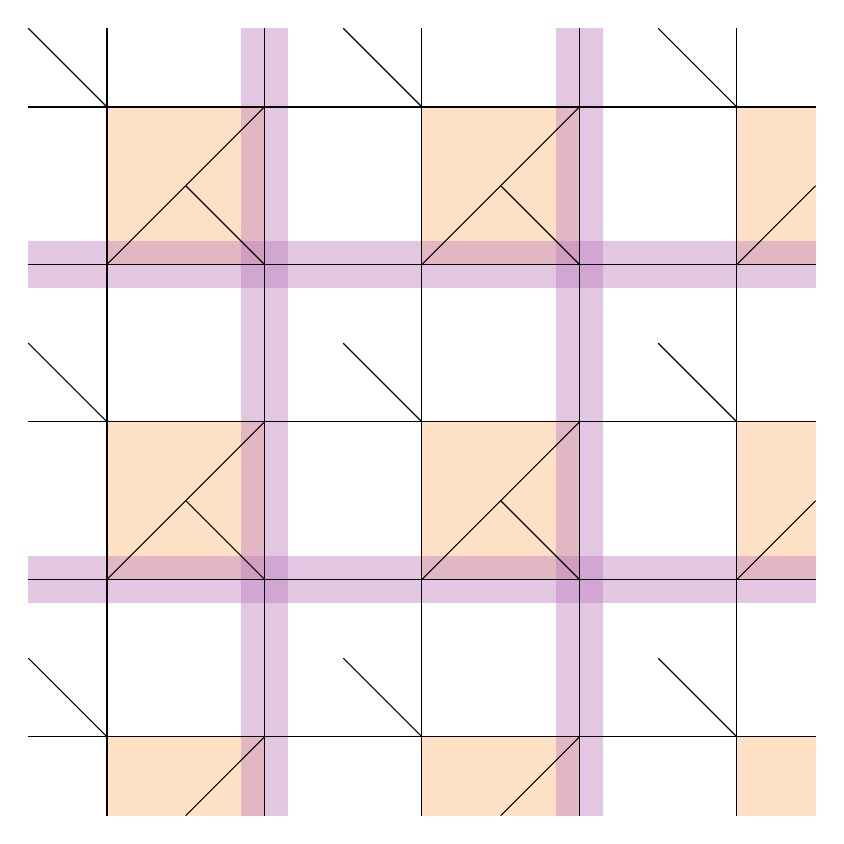
\begin{tikzpicture}
				
					\begin{scope}[xshift = 0cm, yshift=8cm, rotate = -90]
						\lindeca
					\end{scope}
					
					\begin{scope}[yshift = 2cm, rotate = -90]
						\domainwall
					\end{scope}
					
					\begin{scope}[yshift = 6cm, rotate = -90]
						\domainwall
					\end{scope}
					
					\begin{scope}[xshift = 2cm, rotate = 0]
						\domainwall
					\end{scope}
					
					\begin{scope}[xshift = 6cm, rotate = 0]
						\domainwall
					\end{scope}
        				
					\begin{scope}[xshift = 0cm, rotate = 90]
						\vertex
					\end{scope}
					
					\begin{scope}[xshift = 2cm, rotate = 180]
						\vertex
					\end{scope}
					
					\begin{scope}[xshift = 4cm, rotate = 90]
						\vertex
					\end{scope}

					\begin{scope}[xshift = 6cm, rotate = 180]
						\vertex
					\end{scope}

					\begin{scope}[xshift = 8cm, rotate = 90]
						\vertex
					\end{scope}
					
					\begin{scope}[yshift = 2cm, rotate = 0]
						\vertex
					\end{scope}
					
					\begin{scope}[yshift = 2cm, xshift = 2cm, rotate = 90]
						\vertex
					\end{scope}
					
					\begin{scope}[yshift = 2cm, xshift = 4cm, rotate = 0]
						\vertex
					\end{scope}

					\begin{scope}[yshift = 2cm, xshift = 6cm, rotate = 90]
						\vertex
					\end{scope}

					\begin{scope}[yshift = 2cm, xshift = 8cm, rotate = 0]
						\vertex
					\end{scope}
					
					\begin{scope}[yshift = 4cm, rotate = 90]
						\vertex
					\end{scope}
					
					\begin{scope}[yshift = 4cm, xshift = 2cm, rotate = 180]
						\vertex
					\end{scope}
					
					\begin{scope}[yshift = 4cm, xshift = 4cm, rotate = 90]
						\vertex
					\end{scope}

					\begin{scope}[yshift = 4cm, xshift = 6cm, rotate = 180]
						\vertex
					\end{scope}

					\begin{scope}[yshift = 4cm, xshift = 8cm, rotate = 90]
						\vertex
					\end{scope}
					
					\begin{scope}[yshift = 6cm, rotate = 0]
						\vertex
					\end{scope}
					
					\begin{scope}[yshift = 6cm, xshift = 2cm, rotate = 90]
						\vertex
					\end{scope}
					
					\begin{scope}[yshift = 6cm, xshift = 4cm, rotate = 0]
						\vertex
					\end{scope}

					\begin{scope}[yshift = 6cm, xshift = 6cm, rotate = 90]
						\vertex
					\end{scope}

					\begin{scope}[yshift = 6cm, xshift = 8cm, rotate = 0]
						\vertex
					\end{scope}
					
					\begin{scope}[yshift = 8cm, rotate = 90]
						\vertex
					\end{scope}
					
					\begin{scope}[yshift = 8cm, xshift = 2cm, rotate = 180]
						\vertex
					\end{scope}
					
					\begin{scope}[yshift = 8cm, xshift = 4cm, rotate = 90]
						\vertex
					\end{scope}

					\begin{scope}[yshift = 8cm, xshift = 6cm, rotate = 180]
						\vertex				
					\end{scope}

					\begin{scope}[yshift = 8cm, xshift = 8cm, rotate = 90]
						\vertex
					\end{scope}
										
				\end{tikzpicture}
				}
				}
				\caption{Another cm}
				\label{fig:cm:3}
			\end{figure}
			
			%TODO:Explain how to lift the conflict at three-legged vertices.
			Yet another tiling with $cm$ symmetry. It admits domain-wall modes along both directions. It also allows for a linear decay mechanism. Explicit listing yields $n/2+m/2+2$ mechanisms. As shown in Fig.\ref{fig:san:cm:3}, this overcounts the modes by one. This might be because we can express linear decays through domain wall mechanisms, if the two directions are available?
			
\subsection{(cm:4)}
\label{sec:cm:4}

		
			\begin{figure}[!ht]
				\centering{
				\scalebox{0.35}{
				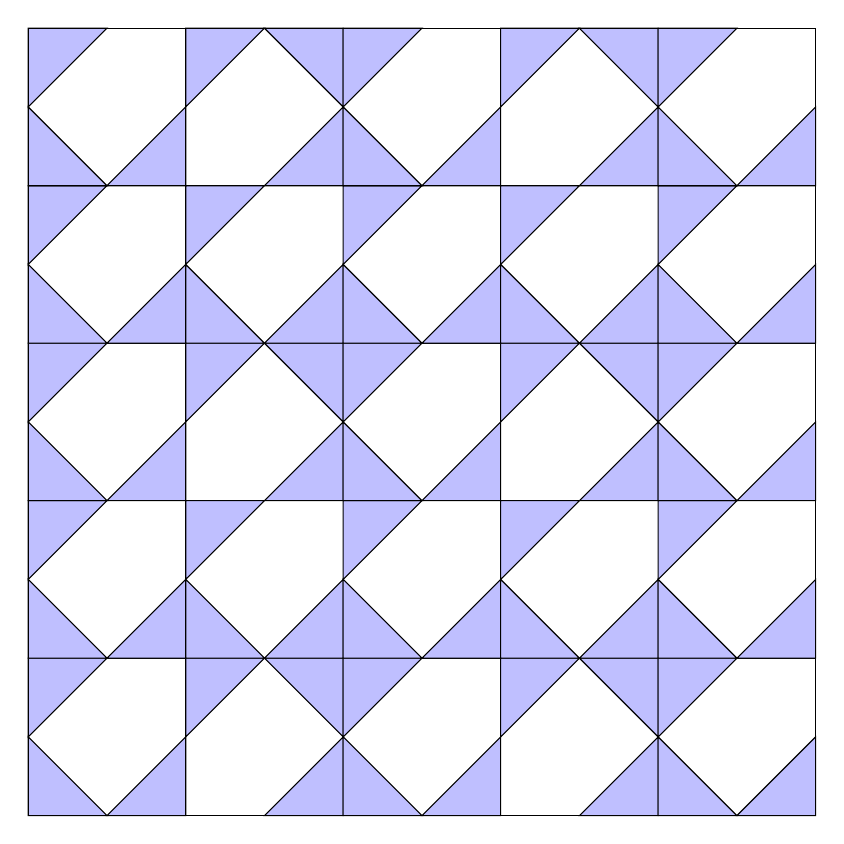
\begin{tikzpicture}
        				
					\bimcell

					\begin{scope}[xshift = 2cm, rotate = 180]
						\bimcell
					\end{scope}
					
					\begin{scope}[xshift = 4cm, rotate = 0]
						\bimcell
					\end{scope}

					\begin{scope}[xshift = 6cm, rotate = 180]
						\bimcell
					\end{scope}

					\begin{scope}[xshift = 8cm, rotate = 0]
						\bimcell
					\end{scope}
					
					\begin{scope}[yshift = 2cm, rotate = 0]
						\bimcell
					\end{scope}
					
					\begin{scope}[yshift = 2cm, xshift = 2cm, rotate = 0]
						\bimcell
					\end{scope}
					
					\begin{scope}[yshift = 2cm, xshift = 4cm, rotate = 0]
						\bimcell
					\end{scope}

					\begin{scope}[yshift = 2cm, xshift = 6cm, rotate = 0]
						\bimcell
					\end{scope}

					\begin{scope}[yshift = 2cm, xshift = 8cm, rotate = 0]
						\bimcell
					\end{scope}
					
					\begin{scope}[yshift = 4cm, rotate = 0]
						\bimcell
					\end{scope}
					
					\begin{scope}[yshift = 4cm, xshift = 2cm, rotate = 180]
						\bimcell
					\end{scope}
					
					\begin{scope}[yshift = 4cm, xshift = 4cm, rotate = 0]
						\bimcell
					\end{scope}

					\begin{scope}[yshift = 4cm, xshift = 6cm, rotate = 180]
						\bimcell
					\end{scope}

					\begin{scope}[yshift = 4cm, xshift = 8cm, rotate = 0]
						\bimcell
					\end{scope}
					
					\begin{scope}[yshift = 6cm, rotate = 0]
						\bimcell
					\end{scope}
					
					\begin{scope}[yshift = 6cm, xshift = 2cm, rotate = 0]
						\bimcell
					\end{scope}
					
					\begin{scope}[yshift = 6cm, xshift = 4cm, rotate = 0]
						\bimcell
					\end{scope}

					\begin{scope}[yshift = 6cm, xshift = 6cm, rotate = 0]
						\bimcell
					\end{scope}

					\begin{scope}[yshift = 6cm, xshift = 8cm, rotate = 0]
						\bimcell
					\end{scope}
					
					\begin{scope}[yshift = 8cm, rotate = 0]
						\bimcell
					\end{scope}
					
					\begin{scope}[yshift = 8cm, xshift = 2cm, rotate = 180]
						\bimcell
					\end{scope}
					
					\begin{scope}[yshift = 8cm, xshift = 4cm, rotate = 0]
						\bimcell
					\end{scope}

					\begin{scope}[yshift = 8cm, xshift = 6cm, rotate = 180]
						\bimcell				
					\end{scope}

					\begin{scope}[yshift = 8cm, xshift = 8cm, rotate = 0]
						\bimcell
					\end{scope}
										
				\end{tikzpicture}
				}
				\qquad
				\qquad
				\scalebox{0.35}{
				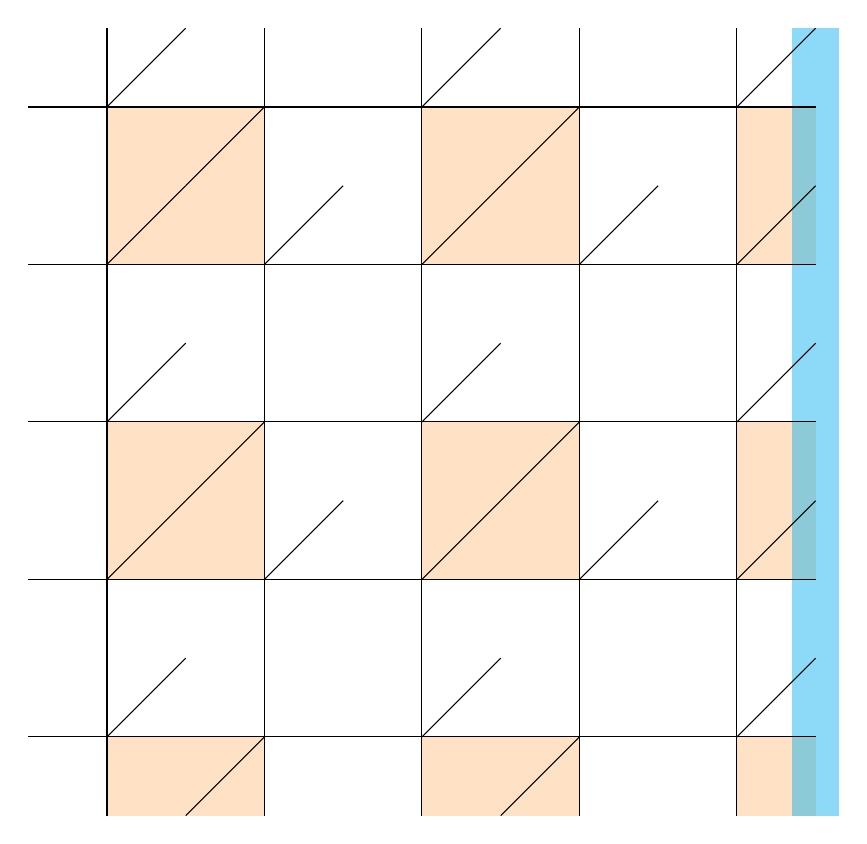
\begin{tikzpicture}
				
					\begin{scope}[xshift = 0cm, yshift=8cm, rotate = -90]
						\lindeca
					\end{scope}
					
					\begin{scope}[xshift = 9cm, rotate = 0]
						\bump
					\end{scope}
        				
					\vertex

					\begin{scope}[xshift = 2cm, rotate = 180]
						\vertex
					\end{scope}
					
					\begin{scope}[xshift = 4cm, rotate = 0]
						\vertex
					\end{scope}

					\begin{scope}[xshift = 6cm, rotate = 180]
						\vertex
					\end{scope}

					\begin{scope}[xshift = 8cm, rotate = 0]
						\vertex
					\end{scope}
					
					\begin{scope}[yshift = 2cm, rotate = 0]
						\vertex
					\end{scope}
					
					\begin{scope}[yshift = 2cm, xshift = 2cm, rotate = 0]
						\vertex
					\end{scope}
					
					\begin{scope}[yshift = 2cm, xshift = 4cm, rotate = 0]
						\vertex
					\end{scope}

					\begin{scope}[yshift = 2cm, xshift = 6cm, rotate = 0]
						\vertex
					\end{scope}

					\begin{scope}[yshift = 2cm, xshift = 8cm, rotate = 0]
						\vertex
					\end{scope}
					
					\begin{scope}[yshift = 4cm, rotate = 0]
						\vertex
					\end{scope}
					
					\begin{scope}[yshift = 4cm, xshift = 2cm, rotate = 180]
						\vertex
					\end{scope}
					
					\begin{scope}[yshift = 4cm, xshift = 4cm, rotate = 0]
						\vertex
					\end{scope}

					\begin{scope}[yshift = 4cm, xshift = 6cm, rotate = 180]
						\vertex
					\end{scope}

					\begin{scope}[yshift = 4cm, xshift = 8cm, rotate = 0]
						\vertex
					\end{scope}
					
					\begin{scope}[yshift = 6cm, rotate = 0]
						\vertex
					\end{scope}
					
					\begin{scope}[yshift = 6cm, xshift = 2cm, rotate = 0]
						\vertex
					\end{scope}
					
					\begin{scope}[yshift = 6cm, xshift = 4cm, rotate = 0]
						\vertex
					\end{scope}

					\begin{scope}[yshift = 6cm, xshift = 6cm, rotate = 0]
						\vertex
					\end{scope}

					\begin{scope}[yshift = 6cm, xshift = 8cm, rotate = 0]
						\vertex
					\end{scope}
					
					\begin{scope}[yshift = 8cm, rotate = 0]
						\vertex
					\end{scope}
					
					\begin{scope}[yshift = 8cm, xshift = 2cm, rotate = 180]
						\vertex
					\end{scope}
					
					\begin{scope}[yshift = 8cm, xshift = 4cm, rotate = 0]
						\vertex
					\end{scope}

					\begin{scope}[yshift = 8cm, xshift = 6cm, rotate = 180]
						\vertex				
					\end{scope}

					\begin{scope}[yshift = 8cm, xshift = 8cm, rotate = 0]
						\vertex
					\end{scope}
										
				\end{tikzpicture}
				}
				}

				\caption{Another cm}
				\label{fig:cm:4}
			\end{figure}
			
			Our final tiling with $cm$ symmetry admits a linear decay sublattice and up to one surface shear, depending on whether $n$ is odd or even. Explicit listing yields $2$ mechanisms.
			
\subsection{(p4m)}
\label{sec:p4m}

		
			\begin{figure}[!ht]
				\centering{
				\scalebox{0.35}{
				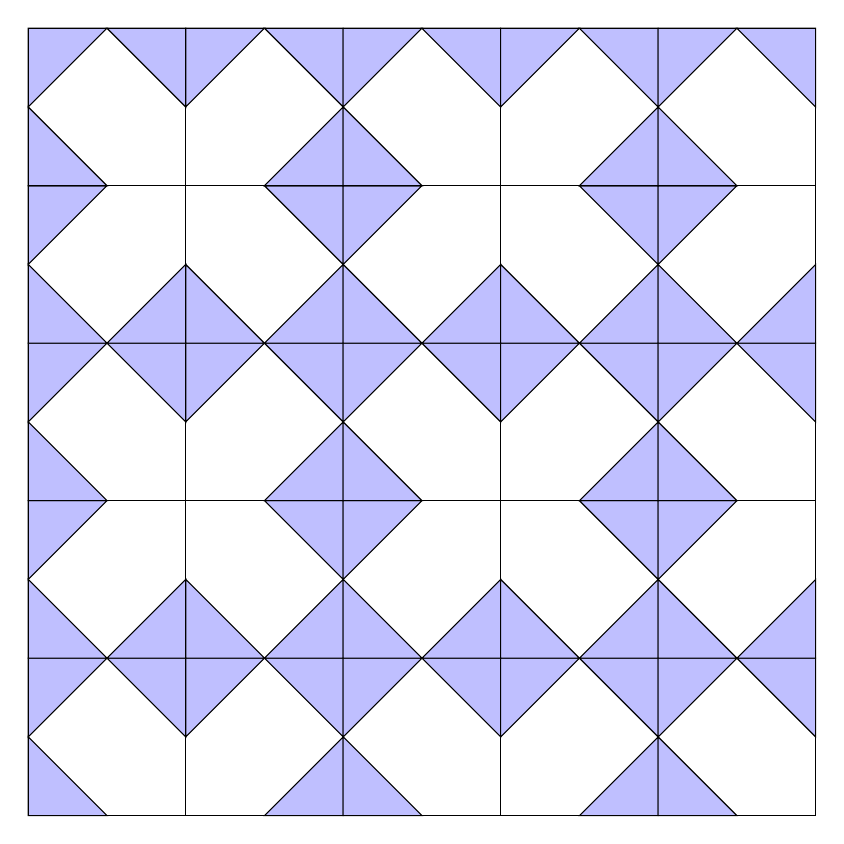
\begin{tikzpicture}
        			
        			\begin{scope}[rotate = 270]
						\bimcell
					\end{scope}

					\begin{scope}[xshift = 2cm, rotate = 180]
						\bimcell
					\end{scope}
					
					\begin{scope}[xshift = 4cm, rotate = 270]
						\bimcell
					\end{scope}

					\begin{scope}[xshift = 6cm, rotate = 180]
						\bimcell
					\end{scope}

					\begin{scope}[xshift = 8cm, rotate = 270]
						\bimcell
					\end{scope}
					
					\begin{scope}[yshift = 2cm, rotate = 0]
						\bimcell
					\end{scope}
					
					\begin{scope}[yshift = 2cm, xshift = 2cm, rotate = 90]
						\bimcell
					\end{scope}
					
					\begin{scope}[yshift = 2cm, xshift = 4cm, rotate = 0]
						\bimcell
					\end{scope}

					\begin{scope}[yshift = 2cm, xshift = 6cm, rotate = 90]
						\bimcell
					\end{scope}

					\begin{scope}[yshift = 2cm, xshift = 8cm, rotate = 0]
						\bimcell
					\end{scope}
					
					\begin{scope}[yshift = 4cm, rotate = 270]
						\bimcell
					\end{scope}
					
					\begin{scope}[yshift = 4cm, xshift = 2cm, rotate = 180]
						\bimcell
					\end{scope}
					
					\begin{scope}[yshift = 4cm, xshift = 4cm, rotate = 270]
						\bimcell
					\end{scope}

					\begin{scope}[yshift = 4cm, xshift = 6cm, rotate = 180]
						\bimcell
					\end{scope}

					\begin{scope}[yshift = 4cm, xshift = 8cm, rotate = 270]
						\bimcell
					\end{scope}
					
					\begin{scope}[yshift = 6cm, rotate = 0]
						\bimcell
					\end{scope}
					
					\begin{scope}[yshift = 6cm, xshift = 2cm, rotate = 90]
						\bimcell
					\end{scope}
					
					\begin{scope}[yshift = 6cm, xshift = 4cm, rotate = 0]
						\bimcell
					\end{scope}

					\begin{scope}[yshift = 6cm, xshift = 6cm, rotate = 90]
						\bimcell
					\end{scope}

					\begin{scope}[yshift = 6cm, xshift = 8cm, rotate = 0]
						\bimcell
					\end{scope}
					
					\begin{scope}[yshift = 8cm, rotate = 270]
						\bimcell
					\end{scope}
					
					\begin{scope}[yshift = 8cm, xshift = 2cm, rotate = 180]
						\bimcell
					\end{scope}
					
					\begin{scope}[yshift = 8cm, xshift = 4cm, rotate = 270]
						\bimcell
					\end{scope}

					\begin{scope}[yshift = 8cm, xshift = 6cm, rotate = 180]
						\bimcell				
					\end{scope}

					\begin{scope}[yshift = 8cm, xshift = 8cm, rotate = 270]
						\bimcell
					\end{scope}
										
				\end{tikzpicture}
				}
				\qquad
				\qquad
				\scalebox{0.35}{
				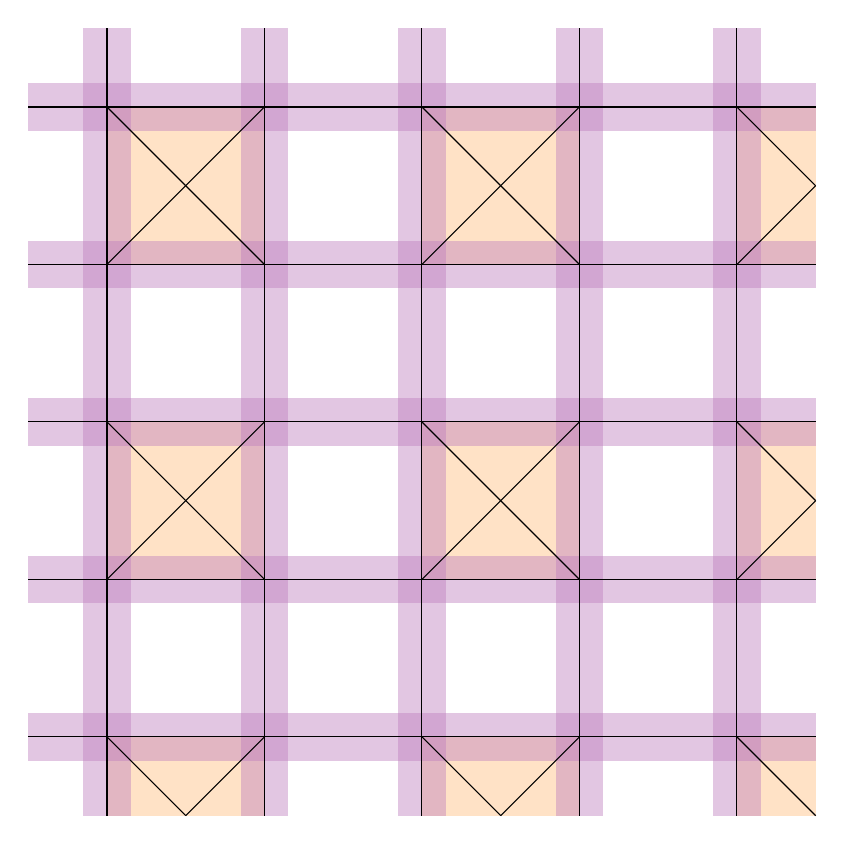
\begin{tikzpicture}
				
					\begin{scope}[xshift = 0cm, yshift=8cm, rotate = -90]
						\lindeca
					\end{scope}
					
					\begin{scope}[yshift = 0cm, rotate = -90]
						\domainwall
					\end{scope}
					
					\begin{scope}[yshift = 2cm, rotate = -90]
						\domainwall
					\end{scope}
					
					\begin{scope}[yshift = 4cm, rotate = -90]
						\domainwall
					\end{scope}
					
					\begin{scope}[yshift = 6cm, rotate = -90]
						\domainwall
					\end{scope}
					
					\begin{scope}[yshift = 8cm, rotate = -90]
						\domainwall
					\end{scope}
					
					\begin{scope}[xshift = 0cm, rotate = 0]
						\domainwall
					\end{scope}
					
					\begin{scope}[xshift = 2cm, rotate = 0]
						\domainwall
					\end{scope}
					
					\begin{scope}[xshift = 4cm, rotate = 0]
						\domainwall
					\end{scope}
					
					\begin{scope}[xshift = 6cm, rotate = 0]
						\domainwall
					\end{scope}
					
					\begin{scope}[xshift = 8cm, rotate = 0]
						\domainwall
					\end{scope}
        			
        			\begin{scope}[rotate = 270]
						\vertex
					\end{scope}

					\begin{scope}[xshift = 2cm, rotate = 180]
						\vertex
					\end{scope}
					
					\begin{scope}[xshift = 4cm, rotate = 270]
						\vertex
					\end{scope}

					\begin{scope}[xshift = 6cm, rotate = 180]
						\vertex
					\end{scope}

					\begin{scope}[xshift = 8cm, rotate = 270]
						\vertex
					\end{scope}
					
					\begin{scope}[yshift = 2cm, rotate = 0]
						\vertex
					\end{scope}
					
					\begin{scope}[yshift = 2cm, xshift = 2cm, rotate = 90]
						\vertex
					\end{scope}
					
					\begin{scope}[yshift = 2cm, xshift = 4cm, rotate = 0]
						\vertex
					\end{scope}

					\begin{scope}[yshift = 2cm, xshift = 6cm, rotate = 90]
						\vertex
					\end{scope}

					\begin{scope}[yshift = 2cm, xshift = 8cm, rotate = 0]
						\vertex
					\end{scope}
					
					\begin{scope}[yshift = 4cm, rotate = 270]
						\vertex
					\end{scope}
					
					\begin{scope}[yshift = 4cm, xshift = 2cm, rotate = 180]
						\vertex
					\end{scope}
					
					\begin{scope}[yshift = 4cm, xshift = 4cm, rotate = 270]
						\vertex
					\end{scope}

					\begin{scope}[yshift = 4cm, xshift = 6cm, rotate = 180]
						\vertex
					\end{scope}

					\begin{scope}[yshift = 4cm, xshift = 8cm, rotate = 270]
						\vertex
					\end{scope}
					
					\begin{scope}[yshift = 6cm, rotate = 0]
						\vertex
					\end{scope}
					
					\begin{scope}[yshift = 6cm, xshift = 2cm, rotate = 90]
						\vertex
					\end{scope}
					
					\begin{scope}[yshift = 6cm, xshift = 4cm, rotate = 0]
						\vertex
					\end{scope}

					\begin{scope}[yshift = 6cm, xshift = 6cm, rotate = 90]
						\vertex
					\end{scope}

					\begin{scope}[yshift = 6cm, xshift = 8cm, rotate = 0]
						\vertex
					\end{scope}
					
					\begin{scope}[yshift = 8cm, rotate = 270]
						\vertex
					\end{scope}
					
					\begin{scope}[yshift = 8cm, xshift = 2cm, rotate = 180]
						\vertex
					\end{scope}
					
					\begin{scope}[yshift = 8cm, xshift = 4cm, rotate = 270]
						\vertex
					\end{scope}

					\begin{scope}[yshift = 8cm, xshift = 6cm, rotate = 180]
						\vertex				
					\end{scope}

					\begin{scope}[yshift = 8cm, xshift = 8cm, rotate = 270]
						\vertex
					\end{scope}
										
				\end{tikzpicture}
				}
				}
				\caption{p4m}
				\label{fig:p4m}
			\end{figure}
			
			This tiling exhibits $p4m$ symmetry. It admits domain-wall modes along both directions. In addition, it allows for a linear decay mechanism. Explicit listing yields $n+m+2$ mechanisms. As shown in Fig.\ref{fig:san:p4m}, this overcounts the modes by two, probably for the same reason as $cm:3$. 

\subsection{Counter-rotations (pmg)}
	\label{sec:crmode}
		
			\begin{figure}[!ht]
				\centering{
				\scalebox{0.35}{
				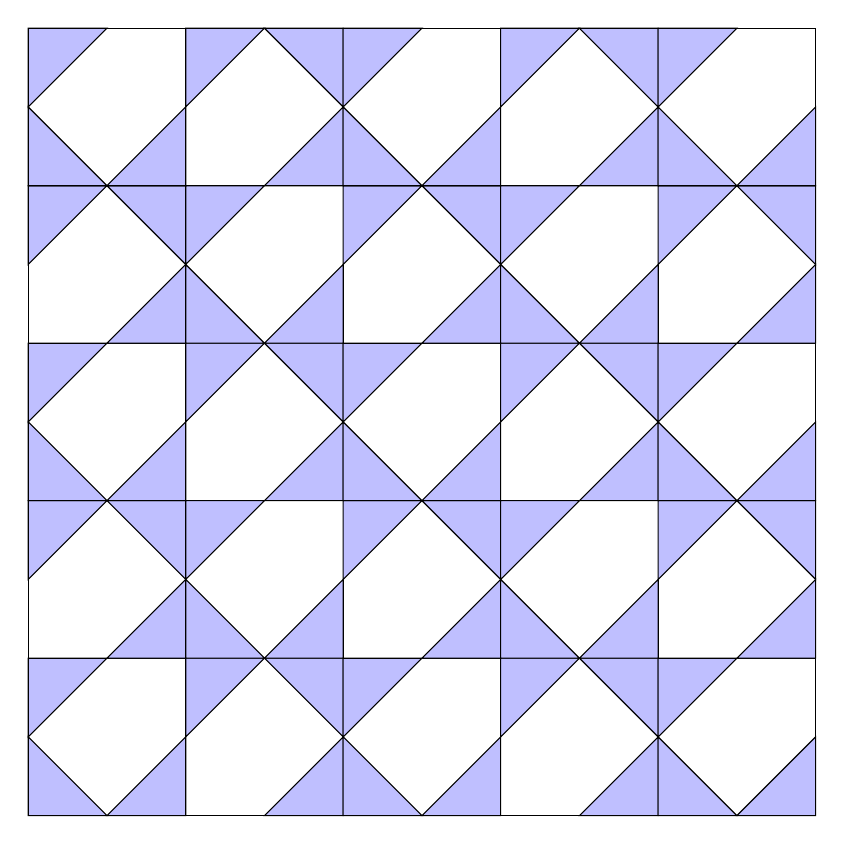
\begin{tikzpicture}
        				
					\bimcell

					\begin{scope}[xshift = 2cm, rotate = 180]
						\bimcell
					\end{scope}
					
					\begin{scope}[xshift = 4cm, rotate = 0]
						\bimcell
					\end{scope}

					\begin{scope}[xshift = 6cm, rotate = 180]
						\bimcell
					\end{scope}

					\begin{scope}[xshift = 8cm, rotate = 0]
						\bimcell
					\end{scope}
					
					\begin{scope}[yshift = 2cm, rotate = 180]
						\bimcell
					\end{scope}
					
					\begin{scope}[yshift = 2cm, xshift = 2cm, rotate = 0]
						\bimcell
					\end{scope}
					
					\begin{scope}[yshift = 2cm, xshift = 4cm, rotate = 180]
						\bimcell
					\end{scope}

					\begin{scope}[yshift = 2cm, xshift = 6cm, rotate = 0]
						\bimcell
					\end{scope}

					\begin{scope}[yshift = 2cm, xshift = 8cm, rotate = 180]
						\bimcell
					\end{scope}
					
					\begin{scope}[yshift = 4cm, rotate = 0]
						\bimcell
					\end{scope}
					
					\begin{scope}[yshift = 4cm, xshift = 2cm, rotate = 180]
						\bimcell
					\end{scope}
					
					\begin{scope}[yshift = 4cm, xshift = 4cm, rotate = 0]
						\bimcell
					\end{scope}

					\begin{scope}[yshift = 4cm, xshift = 6cm, rotate = 180]
						\bimcell
					\end{scope}

					\begin{scope}[yshift = 4cm, xshift = 8cm, rotate = 0]
						\bimcell
					\end{scope}
					
					\begin{scope}[yshift = 6cm, rotate = 180]
						\bimcell
					\end{scope}
					
					\begin{scope}[yshift = 6cm, xshift = 2cm, rotate = 0]
						\bimcell
					\end{scope}
					
					\begin{scope}[yshift = 6cm, xshift = 4cm, rotate = 180]
						\bimcell
					\end{scope}

					\begin{scope}[yshift = 6cm, xshift = 6cm, rotate = 0]
						\bimcell
					\end{scope}

					\begin{scope}[yshift = 6cm, xshift = 8cm, rotate = 180]
						\bimcell
					\end{scope}
					
					\begin{scope}[yshift = 8cm, rotate = 0]
						\bimcell
					\end{scope}
					
					\begin{scope}[yshift = 8cm, xshift = 2cm, rotate = 180]
						\bimcell
					\end{scope}
					
					\begin{scope}[yshift = 8cm, xshift = 4cm, rotate = 0]
						\bimcell
					\end{scope}

					\begin{scope}[yshift = 8cm, xshift = 6cm, rotate = 180]
						\bimcell				
					\end{scope}

					\begin{scope}[yshift = 8cm, xshift = 8cm, rotate = 0]
						\bimcell
					\end{scope}
										
				\end{tikzpicture}
				}
				\qquad
				\qquad
				\scalebox{0.35}{
				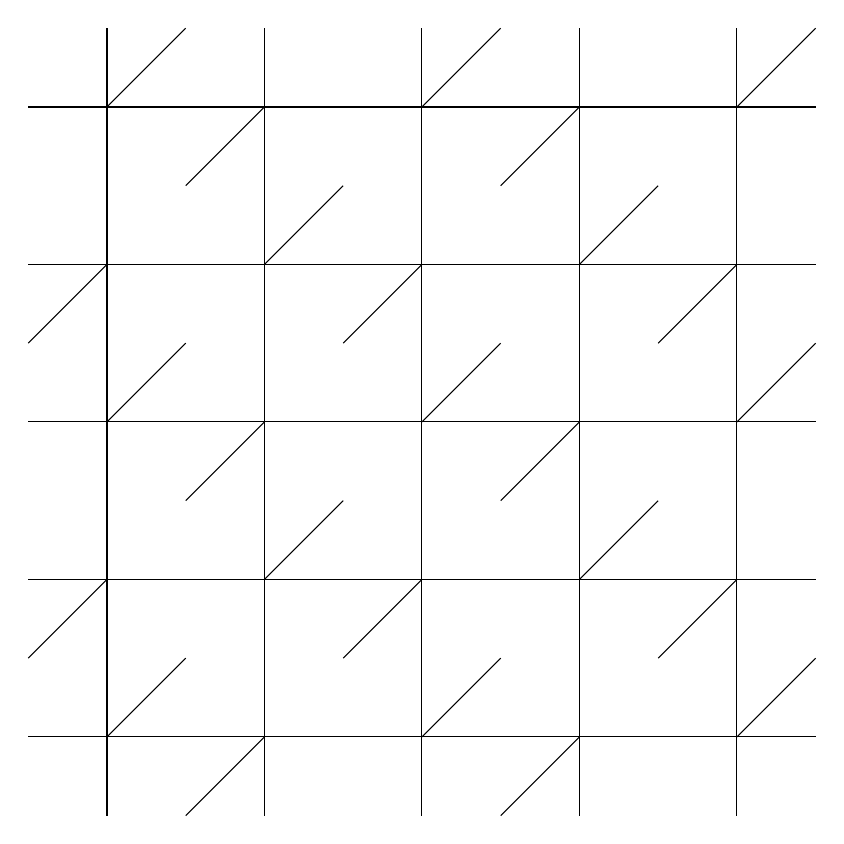
\begin{tikzpicture}
        			
					\vertex

					\begin{scope}[xshift = 2cm, rotate = 180]
						\vertex
					\end{scope}
					
					\begin{scope}[xshift = 4cm, rotate = 0]
						\vertex
					\end{scope}

					\begin{scope}[xshift = 6cm, rotate = 180]
						\vertex
					\end{scope}

					\begin{scope}[xshift = 8cm, rotate = 0]
						\vertex
					\end{scope}
					
					\begin{scope}[yshift = 2cm, rotate = 180]
						\vertex
					\end{scope}
					
					\begin{scope}[yshift = 2cm, xshift = 2cm, rotate = 0]
						\vertex
					\end{scope}
					
					\begin{scope}[yshift = 2cm, xshift = 4cm, rotate = 180]
						\vertex
					\end{scope}

					\begin{scope}[yshift = 2cm, xshift = 6cm, rotate = 0]
						\vertex
					\end{scope}

					\begin{scope}[yshift = 2cm, xshift = 8cm, rotate = 180]
						\vertex
					\end{scope}
					
					\begin{scope}[yshift = 4cm, rotate = 0]
						\vertex
					\end{scope}
					
					\begin{scope}[yshift = 4cm, xshift = 2cm, rotate = 180]
						\vertex
					\end{scope}
					
					\begin{scope}[yshift = 4cm, xshift = 4cm, rotate = 0]
						\vertex
					\end{scope}

					\begin{scope}[yshift = 4cm, xshift = 6cm, rotate = 180]
						\vertex
					\end{scope}

					\begin{scope}[yshift = 4cm, xshift = 8cm, rotate = 0]
						\vertex
					\end{scope}
					
					\begin{scope}[yshift = 6cm, rotate = 180]
						\vertex
					\end{scope}
					
					\begin{scope}[yshift = 6cm, xshift = 2cm, rotate = 0]
						\vertex
					\end{scope}
					
					\begin{scope}[yshift = 6cm, xshift = 4cm, rotate = 180]
						\vertex
					\end{scope}

					\begin{scope}[yshift = 6cm, xshift = 6cm, rotate = 0]
						\vertex
					\end{scope}

					\begin{scope}[yshift = 6cm, xshift = 8cm, rotate = 180]
						\vertex
					\end{scope}
					
					\begin{scope}[yshift = 8cm, rotate = 0]
						\vertex
					\end{scope}
					
					\begin{scope}[yshift = 8cm, xshift = 2cm, rotate = 180]
						\vertex
					\end{scope}
					
					\begin{scope}[yshift = 8cm, xshift = 4cm, rotate = 0]
						\vertex
					\end{scope}

					\begin{scope}[yshift = 8cm, xshift = 6cm, rotate = 180]
						\vertex				
					\end{scope}

					\begin{scope}[yshift = 8cm, xshift = 8cm, rotate = 0]
						\vertex
					\end{scope}
										
				\end{tikzpicture}
				}
				}
				\caption{A tiling that only admits the counter-rotating squares mechaism.}
				\label{fig:crmodes}
			\end{figure}
			
			This tiling exhibits $pmg$ symmetry. It is unimodal, only admitting counter-rotations.
			
			
\subsection{(pmg:2)}
\label{sec:pmg:2}

		
			\begin{figure}[!ht]
				\centering{
				\scalebox{0.35}{
				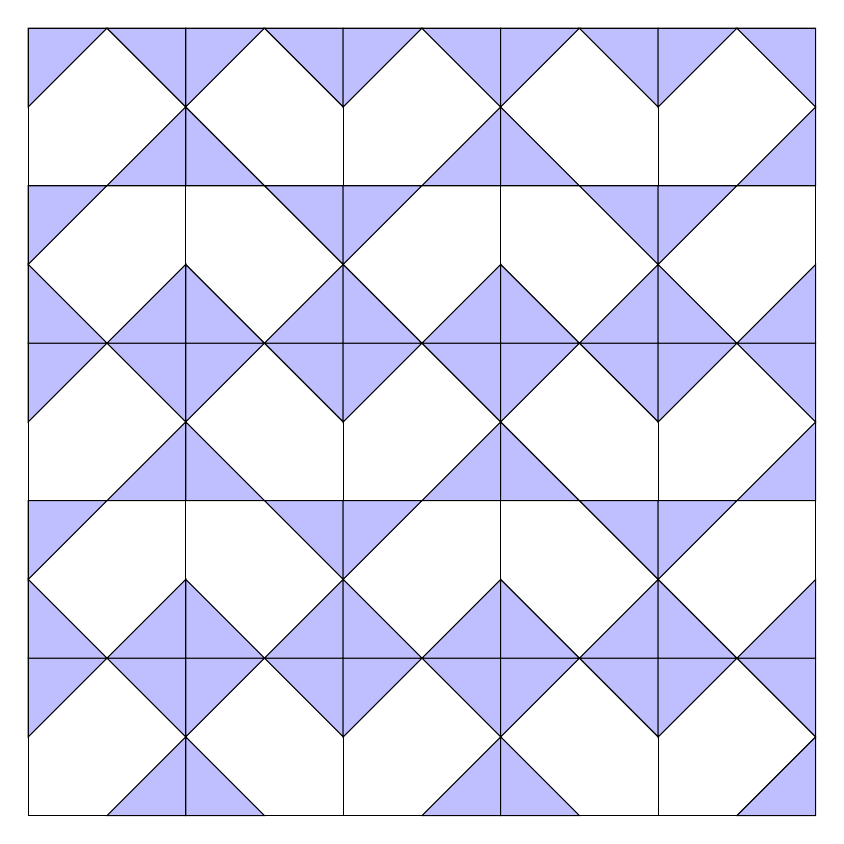
\begin{tikzpicture}
        			
        			\begin{scope}[rotate = 180]
						\bimcell
					\end{scope}

					\begin{scope}[xshift = 2cm, rotate = 270]
						\bimcell
					\end{scope}
					
					\begin{scope}[xshift = 4cm, rotate = 180]
						\bimcell
					\end{scope}

					\begin{scope}[xshift = 6cm, rotate = 270]
						\bimcell
					\end{scope}

					\begin{scope}[xshift = 8cm, rotate = 180]
						\bimcell
					\end{scope}
					
					\begin{scope}[yshift = 2cm, rotate = 0]
						\bimcell
					\end{scope}
					
					\begin{scope}[yshift = 2cm, xshift = 2cm, rotate = 90]
						\bimcell
					\end{scope}
					
					\begin{scope}[yshift = 2cm, xshift = 4cm, rotate = 0]
						\bimcell
					\end{scope}

					\begin{scope}[yshift = 2cm, xshift = 6cm, rotate = 90]
						\bimcell
					\end{scope}

					\begin{scope}[yshift = 2cm, xshift = 8cm, rotate = 0]
						\bimcell
					\end{scope}
					
					\begin{scope}[yshift = 4cm, rotate = 180]
						\bimcell
					\end{scope}
					
					\begin{scope}[yshift = 4cm, xshift = 2cm, rotate = 270]
						\bimcell
					\end{scope}
					
					\begin{scope}[yshift = 4cm, xshift = 4cm, rotate = 180]
						\bimcell
					\end{scope}

					\begin{scope}[yshift = 4cm, xshift = 6cm, rotate = 270]
						\bimcell
					\end{scope}

					\begin{scope}[yshift = 4cm, xshift = 8cm, rotate = 180]
						\bimcell
					\end{scope}
					
					\begin{scope}[yshift = 6cm, rotate = 0]
						\bimcell
					\end{scope}
					
					\begin{scope}[yshift = 6cm, xshift = 2cm, rotate = 90]
						\bimcell
					\end{scope}
					
					\begin{scope}[yshift = 6cm, xshift = 4cm, rotate = 0]
						\bimcell
					\end{scope}

					\begin{scope}[yshift = 6cm, xshift = 6cm, rotate = 90]
						\bimcell
					\end{scope}

					\begin{scope}[yshift = 6cm, xshift = 8cm, rotate = 0]
						\bimcell
					\end{scope}
					
					\begin{scope}[yshift = 8cm, rotate = 180]
						\bimcell
					\end{scope}
					
					\begin{scope}[yshift = 8cm, xshift = 2cm, rotate = 270]
						\bimcell
					\end{scope}
					
					\begin{scope}[yshift = 8cm, xshift = 4cm, rotate = 180]
						\bimcell
					\end{scope}

					\begin{scope}[yshift = 8cm, xshift = 6cm, rotate = 270]
						\bimcell				
					\end{scope}

					\begin{scope}[yshift = 8cm, xshift = 8cm, rotate = 180]
						\bimcell
					\end{scope}
										
				\end{tikzpicture}
				}
				\qquad
				\qquad
				\scalebox{0.35}{
				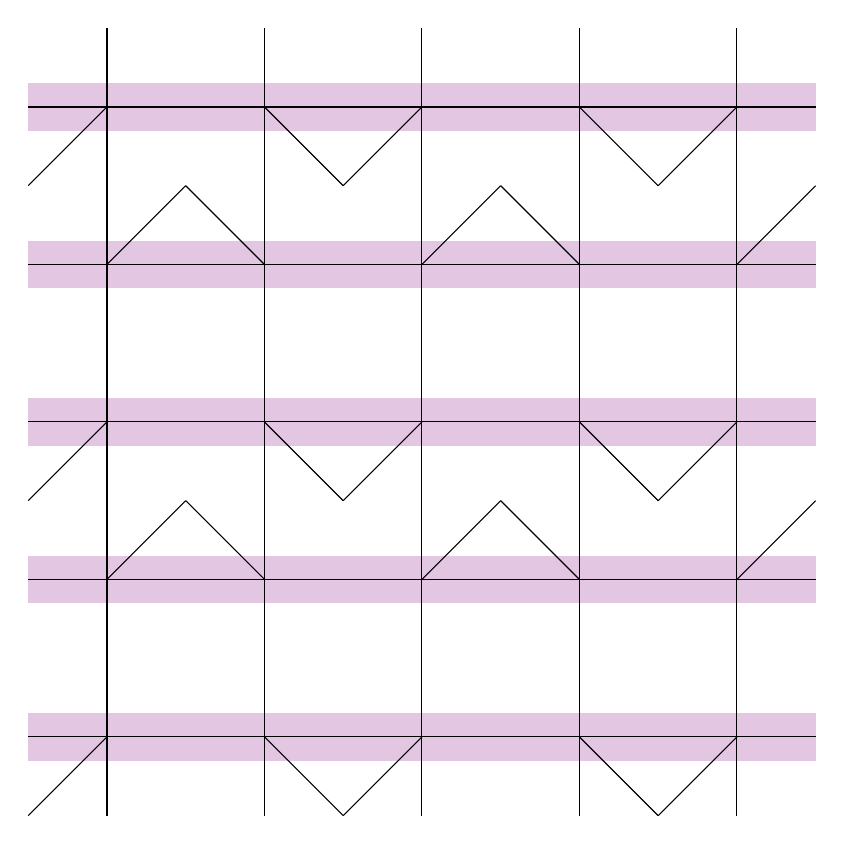
\begin{tikzpicture}
					
					\begin{scope}[yshift = 0cm, rotate = -90]
						\domainwall
					\end{scope}
					
					\begin{scope}[yshift = 2cm, rotate = -90]
						\domainwall
					\end{scope}
					
					\begin{scope}[yshift = 4cm, rotate = -90]
						\domainwall
					\end{scope}
					
					\begin{scope}[yshift = 6cm, rotate = -90]
						\domainwall
					\end{scope}
					
					\begin{scope}[yshift = 8cm, rotate = -90]
						\domainwall
					\end{scope}
        			
        			\begin{scope}[rotate = 180]
						\vertex
					\end{scope}

					\begin{scope}[xshift = 2cm, rotate = 270]
						\vertex
					\end{scope}
					
					\begin{scope}[xshift = 4cm, rotate = 180]
						\vertex
					\end{scope}

					\begin{scope}[xshift = 6cm, rotate = 270]
						\vertex
					\end{scope}

					\begin{scope}[xshift = 8cm, rotate = 180]
						\vertex
					\end{scope}
					
					\begin{scope}[yshift = 2cm, rotate = 0]
						\vertex
					\end{scope}
					
					\begin{scope}[yshift = 2cm, xshift = 2cm, rotate = 90]
						\vertex
					\end{scope}
					
					\begin{scope}[yshift = 2cm, xshift = 4cm, rotate = 0]
						\vertex
					\end{scope}

					\begin{scope}[yshift = 2cm, xshift = 6cm, rotate = 90]
						\vertex
					\end{scope}

					\begin{scope}[yshift = 2cm, xshift = 8cm, rotate = 0]
						\vertex
					\end{scope}
					
					\begin{scope}[yshift = 4cm, rotate = 180]
						\vertex
					\end{scope}
					
					\begin{scope}[yshift = 4cm, xshift = 2cm, rotate = 270]
						\vertex
					\end{scope}
					
					\begin{scope}[yshift = 4cm, xshift = 4cm, rotate = 180]
						\vertex
					\end{scope}

					\begin{scope}[yshift = 4cm, xshift = 6cm, rotate = 270]
						\vertex
					\end{scope}

					\begin{scope}[yshift = 4cm, xshift = 8cm, rotate = 180]
						\vertex
					\end{scope}
					
					\begin{scope}[yshift = 6cm, rotate = 0]
						\vertex
					\end{scope}
					
					\begin{scope}[yshift = 6cm, xshift = 2cm, rotate = 90]
						\vertex
					\end{scope}
					
					\begin{scope}[yshift = 6cm, xshift = 4cm, rotate = 0]
						\vertex
					\end{scope}

					\begin{scope}[yshift = 6cm, xshift = 6cm, rotate = 90]
						\vertex
					\end{scope}

					\begin{scope}[yshift = 6cm, xshift = 8cm, rotate = 0]
						\vertex
					\end{scope}
					
					\begin{scope}[yshift = 8cm, rotate = 180]
						\vertex
					\end{scope}
					
					\begin{scope}[yshift = 8cm, xshift = 2cm, rotate = 270]
						\vertex
					\end{scope}
					
					\begin{scope}[yshift = 8cm, xshift = 4cm, rotate = 180]
						\vertex
					\end{scope}

					\begin{scope}[yshift = 8cm, xshift = 6cm, rotate = 270]
						\vertex				
					\end{scope}

					\begin{scope}[yshift = 8cm, xshift = 8cm, rotate = 180]
						\vertex
					\end{scope}
										
				\end{tikzpicture}
				}
				}
				\caption{Another pmg}
				\label{fig:pmg:2}
			\end{figure}
			
			This tiling also exhibits $pmg$ symmetry. It admits domain-wall modes along one direction but not the other. It seems essentially equivalent to the tiling depicted in Fig.\ref{fig:cm:2}. Explicit listing yields $m+1$ mechanisms.
			
			
	\subsection{Linear decay modes (p4g)}
		\label{sec:lindecay}

		
			\begin{figure}[!ht]
				\centering{
				\scalebox{0.35}{
				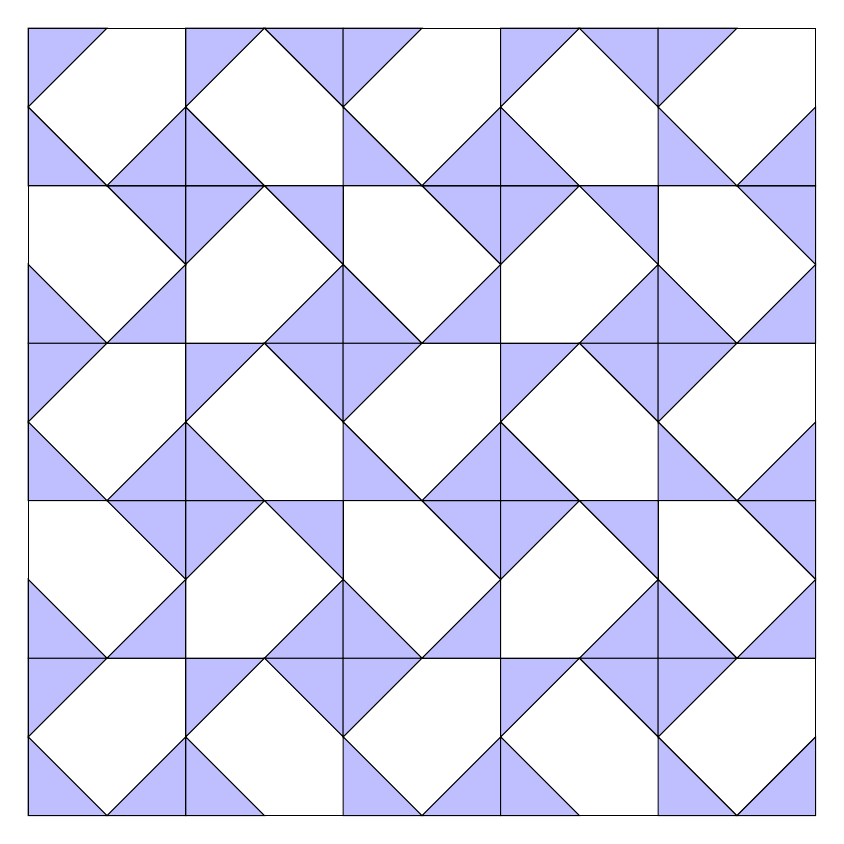
\begin{tikzpicture}
        				
					\bimcell

					\begin{scope}[xshift = 2cm, rotate = 270]
						\bimcell
					\end{scope}
					
					\begin{scope}[xshift = 4cm, rotate = 0]
						\bimcell
					\end{scope}

					\begin{scope}[xshift = 6cm, rotate = 270]
						\bimcell
					\end{scope}

					\begin{scope}[xshift = 8cm, rotate = 0]
						\bimcell
					\end{scope}
					
					\begin{scope}[yshift = 2cm, rotate = 90]
						\bimcell
					\end{scope}
					
					\begin{scope}[yshift = 2cm, xshift = 2cm, rotate = 180]
						\bimcell
					\end{scope}
					
					\begin{scope}[yshift = 2cm, xshift = 4cm, rotate = 90]
						\bimcell
					\end{scope}

					\begin{scope}[yshift = 2cm, xshift = 6cm, rotate = 180]
						\bimcell
					\end{scope}

					\begin{scope}[yshift = 2cm, xshift = 8cm, rotate = 90]
						\bimcell
					\end{scope}
					
					\begin{scope}[yshift = 4cm, rotate = 0]
						\bimcell
					\end{scope}
					
					\begin{scope}[yshift = 4cm, xshift = 2cm, rotate = 270]
						\bimcell
					\end{scope}
					
					\begin{scope}[yshift = 4cm, xshift = 4cm, rotate = 0]
						\bimcell
					\end{scope}

					\begin{scope}[yshift = 4cm, xshift = 6cm, rotate = 270]
						\bimcell
					\end{scope}

					\begin{scope}[yshift = 4cm, xshift = 8cm, rotate = 0]
						\bimcell
					\end{scope}
					
					\begin{scope}[yshift = 6cm, rotate = 90]
						\bimcell
					\end{scope}
					
					\begin{scope}[yshift = 6cm, xshift = 2cm, rotate = 180]
						\bimcell
					\end{scope}
					
					\begin{scope}[yshift = 6cm, xshift = 4cm, rotate = 90]
						\bimcell
					\end{scope}

					\begin{scope}[yshift = 6cm, xshift = 6cm, rotate = 180]
						\bimcell
					\end{scope}

					\begin{scope}[yshift = 6cm, xshift = 8cm, rotate = 90]
						\bimcell
					\end{scope}
					
					\begin{scope}[yshift = 8cm, rotate = 0]
						\bimcell
					\end{scope}
					
					\begin{scope}[yshift = 8cm, xshift = 2cm, rotate = 270]
						\bimcell
					\end{scope}
					
					\begin{scope}[yshift = 8cm, xshift = 4cm, rotate = 0]
						\bimcell
					\end{scope}

					\begin{scope}[yshift = 8cm, xshift = 6cm, rotate = 270]
						\bimcell				
					\end{scope}

					\begin{scope}[yshift = 8cm, xshift = 8cm, rotate = 0]
						\bimcell
					\end{scope}
										
				\end{tikzpicture}
				}
				\qquad
				\qquad
				\scalebox{0.35}{
				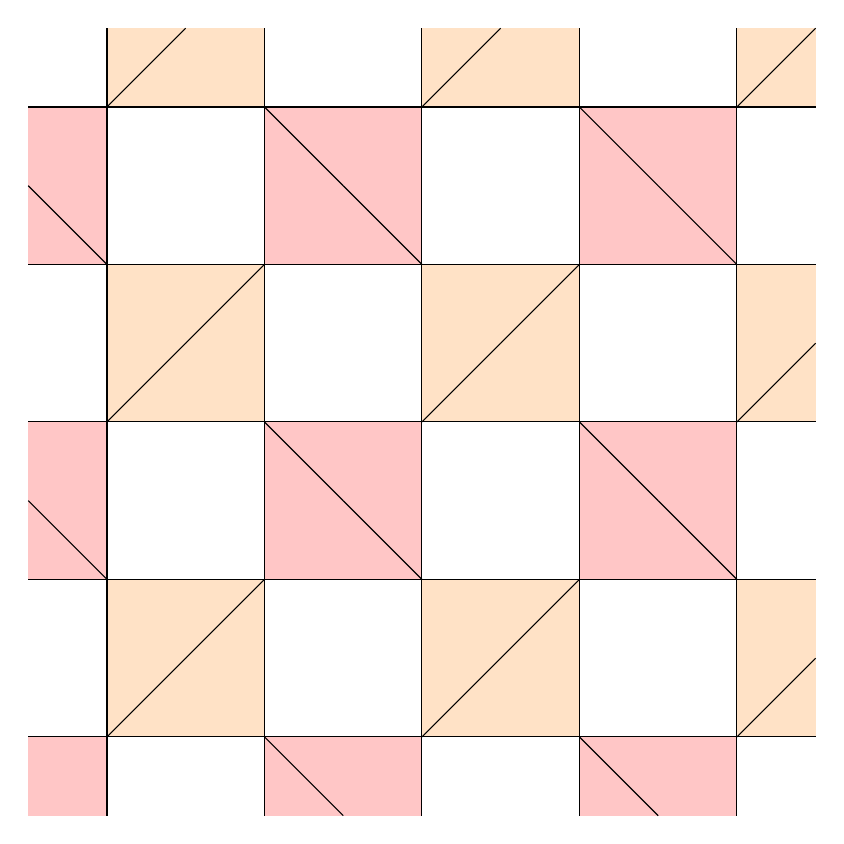
\begin{tikzpicture}
				
					\lindeca
					
					\begin{scope}[xshift = 8cm, yshift=8cm, rotate = 180]
						\lindecb
					\end{scope}
        			
					\vertex

					\begin{scope}[xshift = 2cm, rotate = 270]
						\vertex
					\end{scope}
					
					\begin{scope}[xshift = 4cm, rotate = 0]
						\vertex
					\end{scope}

					\begin{scope}[xshift = 6cm, rotate = 270]
						\vertex
					\end{scope}

					\begin{scope}[xshift = 8cm, rotate = 0]
						\vertex
					\end{scope}
					
					\begin{scope}[yshift = 2cm, rotate = 90]
						\vertex
					\end{scope}
					
					\begin{scope}[yshift = 2cm, xshift = 2cm, rotate = 180]
						\vertex
					\end{scope}
					
					\begin{scope}[yshift = 2cm, xshift = 4cm, rotate = 90]
						\vertex
					\end{scope}

					\begin{scope}[yshift = 2cm, xshift = 6cm, rotate = 180]
						\vertex
					\end{scope}

					\begin{scope}[yshift = 2cm, xshift = 8cm, rotate = 90]
						\vertex
					\end{scope}
					
					\begin{scope}[yshift = 4cm, rotate = 0]
						\vertex
					\end{scope}
					
					\begin{scope}[yshift = 4cm, xshift = 2cm, rotate = 270]
						\vertex
					\end{scope}
					
					\begin{scope}[yshift = 4cm, xshift = 4cm, rotate = 0]
						\vertex
					\end{scope}

					\begin{scope}[yshift = 4cm, xshift = 6cm, rotate = 270]
						\vertex
					\end{scope}

					\begin{scope}[yshift = 4cm, xshift = 8cm, rotate = 0]
						\vertex
					\end{scope}
					
					\begin{scope}[yshift = 6cm, rotate = 90]
						\vertex
					\end{scope}
					
					\begin{scope}[yshift = 6cm, xshift = 2cm, rotate = 180]
						\vertex
					\end{scope}
					
					\begin{scope}[yshift = 6cm, xshift = 4cm, rotate = 90]
						\vertex
					\end{scope}

					\begin{scope}[yshift = 6cm, xshift = 6cm, rotate = 180]
						\vertex
					\end{scope}

					\begin{scope}[yshift = 6cm, xshift = 8cm, rotate = 90]
						\vertex
					\end{scope}
					
					\begin{scope}[yshift = 8cm, rotate = 0]
						\vertex
					\end{scope}
					
					\begin{scope}[yshift = 8cm, xshift = 2cm, rotate = 270]
						\vertex
					\end{scope}
					
					\begin{scope}[yshift = 8cm, xshift = 4cm, rotate = 0]
						\vertex
					\end{scope}

					\begin{scope}[yshift = 8cm, xshift = 6cm, rotate = 270]
						\vertex				
					\end{scope}

					\begin{scope}[yshift = 8cm, xshift = 8cm, rotate = 0]
						\vertex
					\end{scope}
										
				\end{tikzpicture}
				}
				}
				\caption{A tiling that admits four floppy modes.}
				\label{fig:lindecay}
			\end{figure}
			
			This tiling exhibits $p4g$ symmetry. It admits two linear decay sublattices. Explicit listing yields $4$ mechanisms. The combinatorial problem in this specific case might have a solution in the litterature, in relation with the orthogonal dimer lattice. Dig deeper.
			
	\subsection{Bigger primitive cells}
		\label{sec:nxnpc}
		
		We discuss the case of bigger primitve cell using an iterative procedure to see whether new types of modes arise. We also discuss realisations of the missing wallpaper groups: $pg$, $pmm$, $pgg$, $cmm$ and $p4$.
			
		
\section{Aperiodic configurations}
\label{sec:aperio}

A further class of arrangements can be investigated, that of non-crystalline configurations. 

\subsection{Random configurations}
\label{sec:randaperio}
			\begin{figure}[!ht]
				\centering{
				\scalebox{0.35}{
				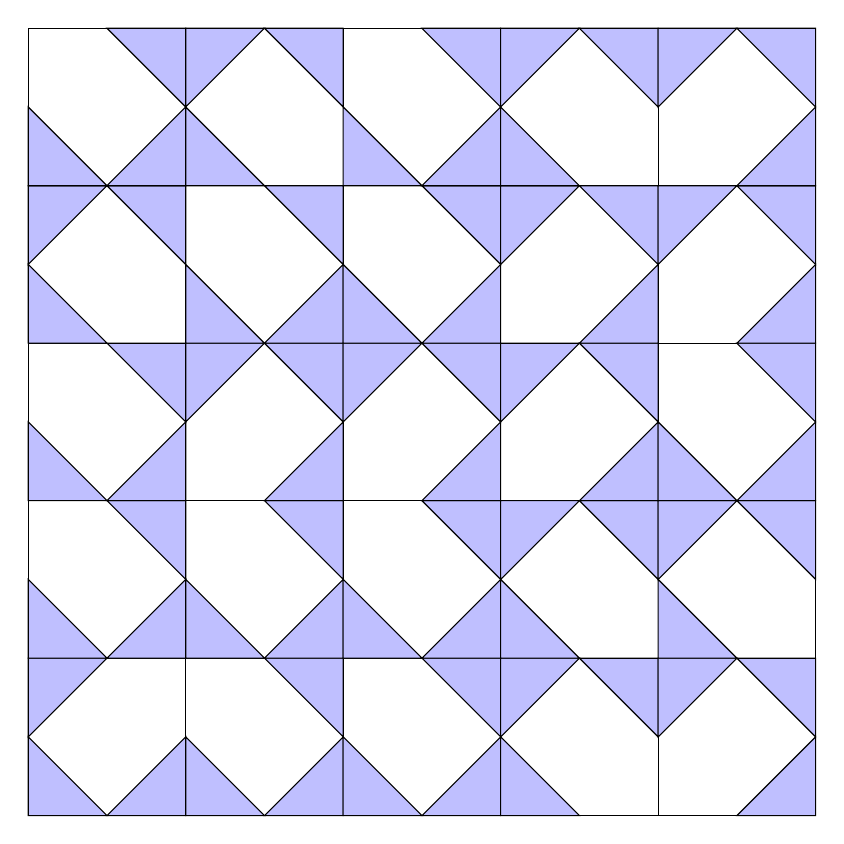
\begin{tikzpicture}
        				
					\bimcell

					\begin{scope}[xshift = 2cm, rotate = 90]
						\bimcell
					\end{scope}
					
					\begin{scope}[xshift = 4cm, rotate = 90]
						\bimcell
					\end{scope}

					\begin{scope}[xshift = 6cm, rotate = 270]
						\bimcell
					\end{scope}

					\begin{scope}[xshift = 8cm, rotate = 180]
						\bimcell
					\end{scope}
					
					\begin{scope}[yshift = 2cm, rotate = 90]
						\bimcell
					\end{scope}
					
					\begin{scope}[yshift = 2cm, xshift = 2cm, rotate = 90]
						\bimcell
					\end{scope}
					
					\begin{scope}[yshift = 2cm, xshift = 4cm, rotate = 90]
						\bimcell
					\end{scope}

					\begin{scope}[yshift = 2cm, xshift = 6cm, rotate = 270]
						\bimcell
					\end{scope}

					\begin{scope}[yshift = 2cm, xshift = 8cm, rotate = 270]
						\bimcell
					\end{scope}
					
					\begin{scope}[yshift = 4cm, rotate = 90]
						\bimcell
					\end{scope}
					
					\begin{scope}[yshift = 4cm, xshift = 2cm, rotate = 180]
						\bimcell
					\end{scope}
					
					\begin{scope}[yshift = 4cm, xshift = 4cm, rotate = 180]
						\bimcell
					\end{scope}

					\begin{scope}[yshift = 4cm, xshift = 6cm, rotate = 180]
						\bimcell
					\end{scope}

					\begin{scope}[yshift = 4cm, xshift = 8cm, rotate = 90]
						\bimcell
					\end{scope}
					
					\begin{scope}[yshift = 6cm, rotate = 270]
						\bimcell
					\end{scope}
					
					\begin{scope}[yshift = 6cm, xshift = 2cm, rotate = 90]
						\bimcell
					\end{scope}
					
					\begin{scope}[yshift = 6cm, xshift = 4cm, rotate = 90]
						\bimcell
					\end{scope}

					\begin{scope}[yshift = 6cm, xshift = 6cm, rotate = 180]
						\bimcell
					\end{scope}

					\begin{scope}[yshift = 6cm, xshift = 8cm, rotate = 180]
						\bimcell
					\end{scope}
					
					\begin{scope}[yshift = 8cm, rotate = 90]
						\bimcell
					\end{scope}
					
					\begin{scope}[yshift = 8cm, xshift = 2cm, rotate = 270]
						\bimcell
					\end{scope}
					
					\begin{scope}[yshift = 8cm, xshift = 4cm, rotate = 90]
						\bimcell
					\end{scope}

					\begin{scope}[yshift = 8cm, xshift = 6cm, rotate = 270]
						\bimcell				
					\end{scope}

					\begin{scope}[yshift = 8cm, xshift = 8cm, rotate = 180]
						\bimcell
					\end{scope}
										
				\end{tikzpicture}
				}
				\qquad
				\qquad
								\scalebox{0.35}{
				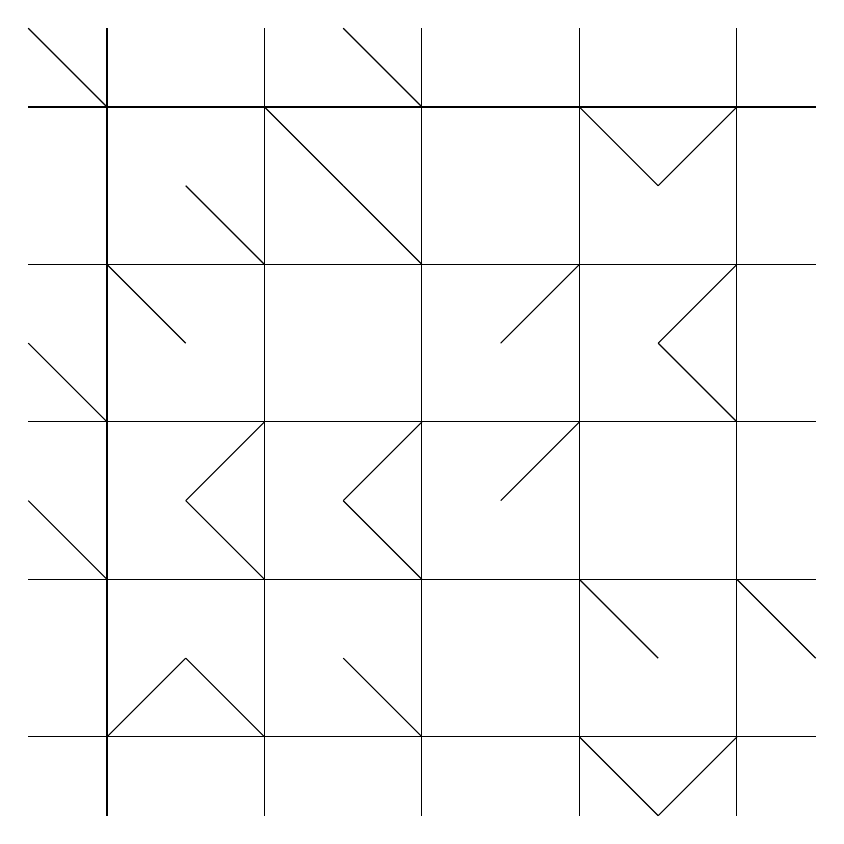
\begin{tikzpicture}
        				
					\vertex

					\begin{scope}[xshift = 2cm, rotate = 90]
						\vertex
					\end{scope}
					
					\begin{scope}[xshift = 4cm, rotate = 90]
						\vertex
					\end{scope}

					\begin{scope}[xshift = 6cm, rotate = 270]
						\vertex
					\end{scope}

					\begin{scope}[xshift = 8cm, rotate = 180]
						\vertex
					\end{scope}
					
					\begin{scope}[yshift = 2cm, rotate = 90]
						\vertex
					\end{scope}
					
					\begin{scope}[yshift = 2cm, xshift = 2cm, rotate = 90]
						\vertex
					\end{scope}
					
					\begin{scope}[yshift = 2cm, xshift = 4cm, rotate = 90]
						\vertex
					\end{scope}

					\begin{scope}[yshift = 2cm, xshift = 6cm, rotate = 270]
						\vertex
					\end{scope}

					\begin{scope}[yshift = 2cm, xshift = 8cm, rotate = 270]
						\vertex
					\end{scope}
					
					\begin{scope}[yshift = 4cm, rotate = 90]
						\vertex
					\end{scope}
					
					\begin{scope}[yshift = 4cm, xshift = 2cm, rotate = 180]
						\vertex
					\end{scope}
					
					\begin{scope}[yshift = 4cm, xshift = 4cm, rotate = 180]
						\vertex
					\end{scope}

					\begin{scope}[yshift = 4cm, xshift = 6cm, rotate = 180]
						\vertex
					\end{scope}

					\begin{scope}[yshift = 4cm, xshift = 8cm, rotate = 90]
						\vertex
					\end{scope}
					
					\begin{scope}[yshift = 6cm, rotate = 270]
						\vertex
					\end{scope}
					
					\begin{scope}[yshift = 6cm, xshift = 2cm, rotate = 90]
						\vertex
					\end{scope}
					
					\begin{scope}[yshift = 6cm, xshift = 4cm, rotate = 90]
						\vertex
					\end{scope}

					\begin{scope}[yshift = 6cm, xshift = 6cm, rotate = 180]
						\vertex
					\end{scope}

					\begin{scope}[yshift = 6cm, xshift = 8cm, rotate = 180]
						\vertex
					\end{scope}
					
					\begin{scope}[yshift = 8cm, rotate = 90]
						\vertex
					\end{scope}
					
					\begin{scope}[yshift = 8cm, xshift = 2cm, rotate = 270]
						\vertex
					\end{scope}
					
					\begin{scope}[yshift = 8cm, xshift = 4cm, rotate = 90]
						\vertex
					\end{scope}

					\begin{scope}[yshift = 8cm, xshift = 6cm, rotate = 270]
						\vertex				
					\end{scope}

					\begin{scope}[yshift = 8cm, xshift = 8cm, rotate = 180]
						\vertex
					\end{scope}
										
				\end{tikzpicture}
				}
				}
				\caption{A random tiling.}
				\label{fig:randaperio}
			\end{figure}
			
			We first consider the generic random case, to understand the generic properties of configurations. As Fig.\ref{randommodes} shows, random configurations typically admit only counter-rotations.
			
\subsection{Ordered aperiodic configurations}
\label{sec:aperiorder}
		
		Can we realize some rosette groups that are forbidden by the crystallographic restriction theorem through aperiodic tilings? These configurations might admit non-trivial modes.

\chapter{Numerical and experimental validation}

\section{Compatibility matrix}

	We conduct a sanity check by computing the size of the compatibility matrix kernel on 11 tesselations for various sizes, in order to confirm the above analysis.
	
		\begin{figure}[!ht]
				\centering{
				\includegraphics[width=0.5\linewidth]{/home/aleksi/Desktop/Metacombinatorial/results/figures/sanitycheck/p1.png}
				}
				\caption{Size dependency of the number of zero modes for the $p1$ tiling.}
				\label{fig:san:p1}
			\end{figure}
			
	
		\begin{figure}[!ht]
				\centering{
				\includegraphics[width=0.5\linewidth]{/home/aleksi/Desktop/Metacombinatorial/results/figures/sanitycheck/p2.png}
				}
				\caption{Size dependency of the number of zero modes for the $p2$ tiling.}
				\label{fig:san:p2}
			\end{figure}
			
	
		\begin{figure}[!ht]
				\centering{
				\includegraphics[width=0.5\linewidth]{/home/aleksi/Desktop/Metacombinatorial/results/figures/sanitycheck/pm.png}
				}
				\caption{Size dependency of the number of zero modes for the $pm$ tiling.}
				\label{fig:san:pm}
			\end{figure}

	
		\begin{figure}[!ht]
				\centering{
				\includegraphics[width=0.5\linewidth]{/home/aleksi/Desktop/Metacombinatorial/results/figures/sanitycheck/cm_1.png}
				}
				\caption{Size dependency of the number of zero modes for the first $cm$ tiling.}
				\label{fig:san:cm:1}
			\end{figure}

	
		\begin{figure}[!ht]
				\centering{
				\includegraphics[width=0.5\linewidth]{/home/aleksi/Desktop/Metacombinatorial/results/figures/sanitycheck/cm_2.png}
				}
				\caption{Size dependency of the number of zero modes for the second $cm$ tiling.}
				\label{fig:san:cm:2}
			\end{figure}

	
		\begin{figure}[!ht]
				\centering{
				\includegraphics[width=0.5\linewidth]{/home/aleksi/Desktop/Metacombinatorial/results/figures/sanitycheck/cm_3.png}
				}
				\caption{Size dependency of the number of zero modes for the third $cm$ tiling.}
				\label{fig:san:cm:3}
			\end{figure}

	
		\begin{figure}[!ht]
				\centering{
				\includegraphics[width=0.5\linewidth]{/home/aleksi/Desktop/Metacombinatorial/results/figures/sanitycheck/cm_4.png}
				}
				\caption{Size dependency of the number of zero modes for the fourth $cm$ tiling.}
				\label{fig:san:cm:4}
			\end{figure}

	
		\begin{figure}[!ht]
				\centering{
				\includegraphics[width=0.5\linewidth]{/home/aleksi/Desktop/Metacombinatorial/results/figures/sanitycheck/p4m.png}
				}
				\caption{Size dependency of the number of zero modes for the $p4m$ tiling.}
				\label{fig:san:p4m}
			\end{figure}

	
		\begin{figure}[!ht]
				\centering{
				\includegraphics[width=0.5\linewidth]{/home/aleksi/Desktop/Metacombinatorial/results/figures/sanitycheck/pmg.png}
				}
				\caption{Size dependency of the number of zero modes for the $pmg$ tiling.}
				\label{fig:san:pmg:1}
			\end{figure}
			
			
		\begin{figure}[!ht]
				\centering{
				\includegraphics[width=0.5\linewidth]{/home/aleksi/Desktop/Metacombinatorial/results/figures/sanitycheck/pmg_2.png}
				}
				\caption{Size dependency of the number of zero modes for the second $pmg$ tiling.}
				\label{fig:san:pmg:2}
			\end{figure}

	
		\begin{figure}[!ht]
				\centering{
				\includegraphics[width=0.5\linewidth]{/home/aleksi/Desktop/Metacombinatorial/results/figures/sanitycheck/p4g.png}
				}
				\caption{Size dependency of the number of zero modes for the $p4g$ tiling.}
				\label{fig:san:p4g}
			\end{figure}
			
		

\section{Finite element simulations}

	What are the nonzero modes? Does the degeneracy of the zero modes survive real hinges?

\section{Elasticity experiments}

	Are there interesting experiments or applications? Do they confirm vertex+FEM? Waveguide? Decay competition?
			
\chapter{Concluding remarks}

	A 3D version of the primitive cell used throughout this work can be created by "emptying" one or several corners of Corentin's unimodal combinatorial cell. Is it necessary to complement the tile set to obain a solvable combinatorial problem?
			
		
		
\renewcommand{\abstractname}{Acknowledgements}
\begin{abstract}
	I would like to thank Corentin for numerous and useful discussions about this project, as well as Tristan of the mechanical workshop for putting up with me as I was learning how to use a laser cutter without burning the building to the ground.
\end{abstract}

\newpage
\bibliography{mybib}{}
\bibliographystyle{hplain}

\begin{appendices}

\chapter{Linearized geometric constraints for triangular lattices}
\label{sec:triderivegeometric}

			\begin{figure}[!ht]
				\centering{
				\scalebox{1}{
				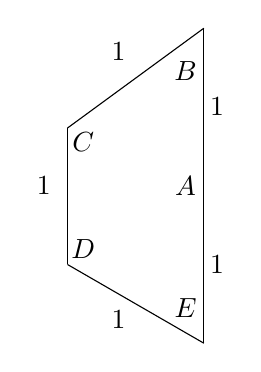
\begin{tikzpicture}
					\node[] at (-0.3,1) {1};
					\node[] at (0.65,-0.7) {1};
					\node[] at (0.65,2.7) {1};
					\node[] at (1.9,2) {1};
					\node[] at (1.9,0) {1};
					
					\node[] at (0.2,0.2) {$D$};
					\node[] at (1.5,-0.55) {$E$};
					\node[] at (0.2,1.55) {$C$};
					\node[] at (1.5,2.45) {$B$};
					\node[] at (1.5,1) {$A$};

					\draw (0,0) -- (0,1.732);
					\draw (0,0) -- (1.732,-1);
					\draw (1.732,3) -- (0,1.732);
					\draw (1.732,3) -- (1.732,1);
					\draw (1.732,-1) -- (1.732,1);

				\end{tikzpicture}
				}}
				\caption{The equilateral pentagon in the reference position.}
				\label{fig:trianglepent}
			\end{figure}
			
			The geometric constraints put forward by the side lengths of the pentagon can be expressed as
			
			\begin{equation}
				A+B+C+D+E = 3\pi,
				\label{eq:trianglesum}
			\end{equation}
			
			\begin{equation}
				2 - 2\cos(A) = 3 - 2 \cos(C) - 2 \cos(D) + 2 \cos(C+D),
				\label{eq:tricosinelaw}
			\end{equation}
			
			\begin{equation}
				\sin(D) - \sin(D+E) = \sin(C) - \sin(C+B).
				\label{eq:trisinelaw}
			\end{equation}
			
			We can linearize these expressions around the
			
			\begin{equation}
				A = \pi + \alpha\quad B = \frac{\pi}{3} + \beta\quad C = \frac{2\pi}{3} + \gamma\quad D = \frac{2\pi}{3} + \delta\quad E = \frac{\pi}{3} + \epsilon
				\label{eq:restriangles}
			\end{equation}
			
			choice of angles, yielding the following system of linear equations,
			
			\begin{equation}
				\begin{pmatrix}
					1 & 1 & 1 & 1 & 1\\
					 & 1 &  &  & 1\\
					 & 1 & 2 & -2 & -1
				\end{pmatrix}
				\begin{pmatrix}
					\alpha\\
					\delta\\
					\epsilon\\
					\beta\\
					\gamma
				\end{pmatrix}
				=\begin{pmatrix}
					0\\
					0\\
					0
				\end{pmatrix}
				\rightarrow
				\begin{pmatrix}
					\alpha\\
					\delta\\
					\epsilon
				\end{pmatrix}
				=
				\begin{pmatrix}
					-2 & -1\\
					   & -1\\
					 1 &  1
				\end{pmatrix}
				\begin{pmatrix}
					\beta\\
					\gamma
				\end{pmatrix}.
				\label{eq:trianglesystem}
			\end{equation}
			
			As expected from the index theorem, there are two free parameters. We express this constraint graphically in Fig.\ref{fig:fundamentalvertices}, by drawing the two modes of our pentagon in a convenient basis. Any linear combination of those two vertices is thus also an acceptable vertex.


				\begin{figure}[!ht]
				\centering{
				\scalebox{1.5}{
				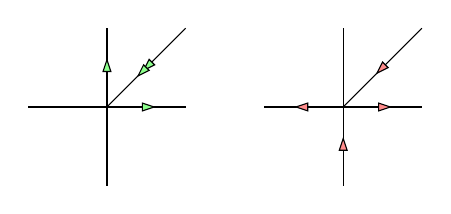
\begin{tikzpicture}
        				
					\vertex
					
					\begin{scope}[xshift = 0.535cm, yshift=0.535cm, rotate = 180]
						\greenarrow
					\end{scope}
					\begin{scope}[xshift = 0.465cm, yshift=0.465cm, rotate = 180]
						\greenarrow
					\end{scope}
					
					\begin{scope}[xshift = 0.5cm, yshift=0cm, rotate = -45]
						\greenarrow
					\end{scope}
					
					\begin{scope}[yshift = 0.5cm, xshift=0cm, rotate = 45]
						\greenarrow
					\end{scope}
					

					\begin{scope}[xshift = 3cm, rotate = 0]
						\vertex
					\end{scope}
					
					\begin{scope}[xshift = 3.5cm, yshift=0.5cm, rotate = 180]
						\redarrow
					\end{scope}
					
					\begin{scope}[xshift = 3.5cm, yshift=0cm, rotate = -45]
						\redarrow
					\end{scope}
					
					\begin{scope}[xshift = 3cm, yshift=-0.5cm, rotate = 45]
						\redarrow
					\end{scope}
					
					\begin{scope}[xshift = 2.5cm, yshift=0cm, rotate = 135]
						\redarrow
					\end{scope}
										
				\end{tikzpicture}
				}
				}
				\caption{Graphical representation of the linearized geometric constraints.}
				\label{fig:trianglevertices}
			\end{figure}

\chapter{Linearized geometric constraints for the inverted prismatic pentagon}
\label{appendix:invprismapent}

			\begin{figure}[!ht]
				\centering{
				\scalebox{0.7}{
				\begin{tikzpicture}
					\draw (0,0) -- (0,4);
					\draw (0,0) -- (4,0);
					\draw (4,4) -- (0,4);
					\draw (4,4) -- (2,2);
					\draw (4,0) -- (2,2);

					
				\end{tikzpicture}
				}}
				\caption{The inverted prismatic pentagon in the reference position.}
				\label{fig:invprismapent}
			\end{figure}
			
			\begin{figure}[!ht]
				\centering{
				\scalebox{1.5}{
				\begin{tikzpicture}
        				
					\vertex

					\begin{scope}[xshift = 3cm, rotate = 0]
						\vertex
					\end{scope}
										
				\end{tikzpicture}
				}
				}
				\caption{Graphical representation of the linearized geometric constraints.}
				\label{fig:invfundamentalvertices}
			\end{figure}
			
%\chapter{Some composite mechanisms}
%\label{appendix:compositevertex}
%				\begin{figure}[!ht]
%				\centering{
%				\scalebox{0.7}{
%				\begin{tikzpicture}
%				
%					\begin{scope}[yshift = 2cm, rotate = 270]
%						\vertex
%						\begin{scope}[xshift = 0cm, yshift=-1cm, rotate = 45]
%							\bigredarrow
%						\end{scope}
%						\begin{scope}[xshift = 0.57cm, yshift=0.57cm, rotate = -180]
%							\biggreenarrow
%						\end{scope}
%						\begin{scope}[xshift = 0.43cm, yshift=0.43cm, rotate = -180]
%							\biggreenarrow
%						\end{scope}
%					\end{scope}
%					
%					\begin{scope}[yshift = 2cm, xshift = 2cm, rotate = 180]
%						\vertex
%						\begin{scope}[xshift = 1cm, yshift=0cm, rotate = 135]
%							\biggreenarrow
%						\end{scope}
%						\begin{scope}[xshift = 0.43cm, yshift=0.43cm, rotate = 0]
%							\biggreenarrow
%						\end{scope}
%						\begin{scope}[xshift = 0.57cm, yshift=0.57cm, rotate = 0]
%							\biggreenarrow
%						\end{scope}
%					\end{scope}
%					
%					\begin{scope}[yshift = 2cm, xshift = 4cm, rotate = 270]
%						\vertex
%						\begin{scope}[xshift = 0cm, yshift=-1cm, rotate = 45]
%							\biggreenarrow
%						\end{scope}
%						\begin{scope}[xshift = 0.57cm, yshift=0.57cm, rotate = -180]
%							\biggreenarrow
%						\end{scope}
%						\begin{scope}[xshift = 0.43cm, yshift=0.43cm, rotate = -180]
%							\biggreenarrow
%						\end{scope}
%					\end{scope}
%
%					\begin{scope}[yshift = 2cm, xshift = 6cm, rotate = 180]
%						\vertex
%						\begin{scope}[xshift = 1cm, yshift=0cm, rotate = 135]
%							\biggreenarrow
%						\end{scope}
%						\begin{scope}[xshift = 0.43cm, yshift=0.43cm, rotate = 0]
%							\biggreenarrow
%						\end{scope}
%						\begin{scope}[xshift = 0.57cm, yshift=0.57cm, rotate = 0]
%							\biggreenarrow
%						\end{scope}
%					\end{scope}
%
%					\begin{scope}[yshift = 2cm, xshift = 8cm, rotate = 270]
%						\vertex
%						\begin{scope}[xshift = 0cm, yshift=-1cm, rotate = 45]
%							\biggreenarrow
%						\end{scope}
%						\begin{scope}[xshift = 0.57cm, yshift=0.57cm, rotate = -180]
%							\biggreenarrow
%						\end{scope}
%						\begin{scope}[xshift = 0.43cm, yshift=0.43cm, rotate = -180]
%							\biggreenarrow
%						\end{scope}
%					\end{scope}
%					
%					\begin{scope}[yshift = 2cm, xshift = 10cm, rotate = 180]
%						\vertex
%						\begin{scope}[xshift = 1cm, yshift=0cm, rotate = 135]
%							\biggreenarrow
%						\end{scope}
%						\begin{scope}[xshift = 0.43cm, yshift=0.43cm, rotate = 0]
%							\biggreenarrow
%						\end{scope}
%						\begin{scope}[xshift = 0.57cm, yshift=0.57cm, rotate = 0]
%							\biggreenarrow
%						\end{scope}
%					\end{scope}
%					
%					\begin{scope}[yshift = 2cm, xshift = 12cm, rotate = 270]
%						\vertex
%						\begin{scope}[xshift = 0cm, yshift=-1cm, rotate = 45]
%							\biggreenarrow
%						\end{scope}
%						\begin{scope}[xshift = 0cm, yshift=1cm, rotate = 45]
%							\biggreenarrow
%						\end{scope}
%						\begin{scope}[xshift = 0.57cm, yshift=0.57cm, rotate = -180]
%							\biggreenarrow
%						\end{scope}
%						\begin{scope}[xshift = 0.43cm, yshift=0.43cm, rotate = -180]
%							\biggreenarrow
%						\end{scope}
%					\end{scope}
%        				
%					\vertex
%						\begin{scope}[yshift = 3cm, rotate = 0]
%							\fixededge
%						\end{scope}
%						
%						\begin{scope}[yshift = 1.14cm, rotate = -135]
%							\biggreenarrow
%						\end{scope}
%						\begin{scope}[yshift = 0.86cm, rotate = -135]
%							\biggreenarrow
%						\end{scope}
%						
%						\begin{scope}[xshift = -1cm, rotate = 135]
%							\biggreenarrow
%						\end{scope}
%
%					\begin{scope}[xshift = 2cm, rotate = 90]
%						\vertex
%						\begin{scope}[xshift = 3cm, rotate = 0]
%							\fixededge
%						\end{scope}
%						\begin{scope}[xshift = 0.86cm, rotate = -45]
%							\biggreenarrow
%						\end{scope}
%						\begin{scope}[xshift = 1.14cm, rotate = -45]
%							\biggreenarrow
%						\end{scope}
%						\begin{scope}[yshift = 1cm, rotate = 45]
%							\biggreenarrow
%						\end{scope}
%					\end{scope}
%					
%					\begin{scope}[xshift = 4cm, rotate = 0]
%						\vertex
%						\begin{scope}[yshift = 3cm, rotate = 0]
%							\fixededge
%						\end{scope}
%						\begin{scope}[yshift = 1.14cm, rotate = -135]
%							\biggreenarrow
%						\end{scope}
%						\begin{scope}[yshift = 0.86cm, rotate = -135]
%							\biggreenarrow
%						\end{scope}
%						\begin{scope}[xshift = -1cm, rotate = 135]
%							\biggreenarrow
%						\end{scope}
%					\end{scope}
%
%					\begin{scope}[xshift = 6cm, rotate = 90]
%						\vertex
%						\begin{scope}[xshift = 3cm, rotate = 0]
%							\fixededge
%						\end{scope}
%						\begin{scope}[xshift = 0.86cm, rotate = -45]
%							\biggreenarrow
%						\end{scope}
%						\begin{scope}[xshift = 1.14cm, rotate = -45]
%							\biggreenarrow
%						\end{scope}
%						\begin{scope}[yshift = 1cm, rotate = 45]
%							\biggreenarrow
%						\end{scope}
%					\end{scope}
%
%					\begin{scope}[xshift = 8cm, rotate = 0]
%						\vertex
%						\begin{scope}[yshift = 3cm, rotate = 0]
%							\fixededge
%						\end{scope}
%						\begin{scope}[yshift = 1.14cm, rotate = -135]
%							\biggreenarrow
%						\end{scope}
%						\begin{scope}[yshift = 0.86cm, rotate = -135]
%							\biggreenarrow
%						\end{scope}
%						\begin{scope}[xshift = -1cm, rotate = 135]
%							\biggreenarrow
%						\end{scope}
%					\end{scope}
%					
%					\begin{scope}[xshift = 10cm, rotate = 90]
%						\vertex
%						\begin{scope}[xshift = 3cm, rotate = 0]
%							\fixededge
%						\end{scope}
%						\begin{scope}[xshift = 0.86cm, rotate = -45]
%							\biggreenarrow
%						\end{scope}
%						\begin{scope}[xshift = 1.14cm, rotate = -45]
%							\biggreenarrow
%						\end{scope}
%						\begin{scope}[yshift = 1cm, rotate = 45]
%							\biggreenarrow
%						\end{scope}
%					\end{scope}
%					
%					\begin{scope}[xshift = 12cm, rotate = 0]
%						\vertex
%						\begin{scope}[yshift = 3cm, rotate = 0]
%							\fixededge
%						\end{scope}
%						\begin{scope}[yshift = 1.14cm, rotate = -135]
%							\biggreenarrow
%						\end{scope}
%						\begin{scope}[yshift = 0.86cm, rotate = -135]
%							\biggreenarrow
%						\end{scope}
%						\begin{scope}[xshift = -1cm, rotate = 135]
%							\biggreenarrow
%						\end{scope}
%						\textbf{\begin{scope}[xshift = 1cm, rotate = 135]
%							\biggreenarrow
%						\end{scope}}
%					\end{scope}
%								
%				\end{tikzpicture}
%				}
%				}
%				\caption{Vertex configuration of an activated source mechanism. The red points denote fixed angles.}
%				\label{fig:xbox}
%			\end{figure}
			
\chapter{Basic states of self-stress}
\label{appendix:selfstress}

	We will now identify a few localized states of self-stress that can occur within our tesselations, in order to obtain an lower bound on the number of mechanisms for a given tiling.
	
			\begin{figure}[!ht]
				\centering{
				\scalebox{1}{
				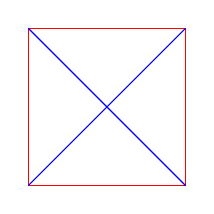
\begin{tikzpicture}
				
					\draw[red] (0,0) -- (0,2);
					\draw[red] (0,0) -- (2,0);
					\draw[red] (2,2) -- (0,2);
					\draw[red] (2,2) -- (2,0);
					\draw[blue] (2,2) -- (0,0);
					\draw[blue] (2,0) -- (0,2);

				\end{tikzpicture}
				}}
				\caption{The textbook example of a state of self-stress.}
				\label{fig:stress1}
			\end{figure}
			
			\begin{figure}[!ht]
				\centering{
				\scalebox{1}{
				\begin{tikzpicture}
				
					\draw[blue] (0,0) -- (0,-2);
					\draw[blue] (0,0) -- (-2,0);
					\draw[blue] (2,2) -- (2,4);
					\draw[blue] (2,2) -- (4,2);
					\draw[blue] (0,2) -- (0,4);
					\draw[blue] (0,2) -- (-2,2);
					\draw[blue] (2,0) -- (2,-2);
					\draw[blue] (2,0) -- (4,0);
					
					\draw[red] (-2,0) -- (0,-2);
					\draw[red] (-2,2) -- (-2,0);
					\draw[red] (4,2) -- (2,4);
					\draw[red] (0,4) -- (2,4);
					\draw[red] (-2,2) -- (0,4);
					\draw[red] (0,-2) -- (2,-2);
					\draw[red] (4,0) -- (2,-2);
					\draw[red] (4,2) -- (4,0);
					
					\draw[blue] (2,2) -- (0,0);
					\draw[blue] (2,0) -- (0,2);

				\end{tikzpicture}
				}}
				\caption{A less trivial state of self-stress.}
				\label{fig:stress2}
			\end{figure}
			
			\begin{figure}[!ht]
				\centering{
				\scalebox{1}{
				\begin{tikzpicture}
				
					\draw[blue] (0,0) -- (0,-2);
					\draw[blue] (0,0) -- (-2,0);
					\draw[blue] (0,2) -- (0,4);
					\draw[blue] (0,2) -- (-2,2);
					
					\draw[red] (-2,0) -- (0,-2);
					\draw[red] (-2,2) -- (-2,0);
					\draw[red] (4,2) -- (4,4);
					\draw[red] (4,-2) -- (4,0);
					\draw[red] (0,4) -- (4,4);
					\draw[red] (-2,2) -- (0,4);
					\draw[red] (0,-2) -- (4,-2);
					
					\draw[blue] (4,4) -- (0,0);
					\draw[blue] (0,2) -- (4,-2);
					
					\draw[red] (4,2) -- (6,0);
					\draw[red] (6,2) -- (4,0);
					
					\draw[blue] (4,2) -- (6,2);
					\draw[blue] (6,0) -- (4,0);
					\draw[blue] (6,0) -- (6,2);

				\end{tikzpicture}
				}}
				\caption{Another one.}
				\label{fig:stress3}
			\end{figure}

\end{appendices}

\end{document}